\section{The Structure of Groups}
In this chapter, we continue our study on group theory to get some depth for certain classes of abelian groups and for various classes of groups that share some desirable properties with abelian groups. We shall always use additive notation in this chapter. We give a dictionary of notations: 
$$
\begin{matrix}
	\mathrm{additive}\ \mathrm{notation}&		\mathrm{multiplicative}\ \mathrm{notation}\\
	a+b&		ab\\
	-a&		a^{-1}\\
	0&		e\\
	na&		a^n\\
	a-b&		ab^{-1}\\
	H+K&		HK\\
	a+H&		aH\\
	G\oplus H&		G\times H\\
	H+K&		H\lor K\\
	\sum_{i\in I}{G_i}&		{\prod}^w_{i\in I}{G_i}\\
	\mathrm{direct}\ \mathrm{sum}&		\mathrm{weak}\ \mathrm{direct}\ \mathrm{product}\\
\end{matrix}
$$
\subsection{Free Abelian Groups}
We shall investigate free objects in the category of abelian groups. First we introduce some terminology.\par
Let $G$ be a group of additive notation. If $X$ is a nonempty subset of $G$, then $\left<X\right>$ contains all \textbf{linear combinations} $n_1x_1+n_2x_2+\cdots+n_kx_k(n_i\in\mathbb{Z},x_i\in X)$. In particular, the cyclic group $\left<x\right>=\{nx:n\in\mathbb{Z}\}$.\par
A \textbf{basis} of an abelian group $F$ is a subset $X$ of $F$ such that $F=\left<X\right>$, and for distinct $x_1,x_2,\cdots,x_k\in X$ and $n_i\in\mathbb{Z}$, 
$$n_1x_1+n_2x_2+\cdots+n_kx_k=0\Rightarrow n_i=0\ \text{for every} \ i.$$
\begin{theorem}
The following conditions on an abelian group $F$ are equivalent.\par
(i) $F$ has a nonempty basis.\par
(ii) $F$ is the (internal) direct sum of a family of infinite cyclic subgroups.\par
(iii) $F$ is isomorphic to a direct sum of copies of the additive group $\mathbb{Z}$ of integers.\par
(iv) There exists a nonempty set $X$ and a function $\iota:X\to F$ with the following property: given an abelian group $G$ and function $f:X\to G$, there exists a unique homomorphism of groups $\overline{f}:F\to G$ such that $\overline{f}\iota=f$. In other words, $F$ is free object in the category of abelian groups.
\end{theorem}
We call the abelian group satisfying conditions above a \textbf{free abelian group}. By definition the trivial group $0$ is the free abelian group on the null set $\emptyset$.
\begin{proof}
(i)$\Rightarrow$(ii): Let $X$ be a basis of $F$, we show that $F=\sum_{x\in X}\left<x\right>$, which is the direct sum of infinite cyclic subgroups (if finite, then there exists some $n\in\mathbb{Z}$ such that $nx=0$, which contradict to the fact that $X$ is a basis). Since $F=\left<X\right>$, we know that $F=\left<\bigcup_{x\in X}x\right>$. Let $x_0\in X$, we consider $\left<x_0\right>\cap\left<\bigcup_{x\in X\setminus\{x_0\}}x\right>$. If $\left<x_0\right>\cap\left<\bigcup_{x\in X\setminus\{x_0\}}x\right>\ne 0$, then there exists some $k_0,k_1,\cdots,k_n$ such that $k_0x_0=k_1x_1+k_2x_2+\cdots+k_nx_n\ne 0$, here $x_i\in X,0\le i\le n$. However, since $X$ is a basis we know that $k_0=k_1=\cdots=k_n=0$, which is a contradiction! Hence by the definition of a direct sum we know that $F=\sum_{x\in X}\left<x\right>$.\par
(ii)$\Rightarrow$(iii): Since $\left<x\right>$ are infinite cyclic groups, then $\left<x\right>\cong\mathbb{Z}$. Hence by theorem 2.69 we know that $F=\sum_{x\in X}\left<x\right>\cong\sum_{|X|}\mathbb{Z}$.
\par
(iii)$\Rightarrow$(i): Let $F\cong\sum\mathbb{Z}$, where $\mathbb{Z}$ are indexed with a set $X$. For each $x\in I$, let $\theta_x$ be the element $\{u_i\}\in\sum\mathbb{Z}$ satisfying $u_i=0$ for $i\ne x$ and $u_x=1$. Therefore it is easy to verify $\{\theta_x\}$ is a basis of $\sum\mathbb{Z}$. Then by $F\cong\sum\mathbb{Z}$ we may define a basis of $F$ by isomorphism.\par
(i)$\Rightarrow$(iv): Let $X$ be the basis of $F$ and $\iota:X\to F$ be the inclusion map. Given $G$ abelian and map $f:X\to G$, we define $\overline{f}:F\to G$ by $\sum_{i\in I}n_ix_i\mapsto\sum_{i\in I}n_if(x_i)$. We first show that $\overline{f}$ is well-defined. Let $x\in F$, then $x=\sum_{i\in I}n_ix_i$ for some $n_i$ and $x_i$. Now if $x=\sum_{i\in I}m_ix_i$, then $\sum_{i\in I}(n_i-m_i)x_i=0$, hence $n_i=m_i$ since $X$ is a basis of $F$. It is easy to show that $\overline{f}$ is a homomorphism since $F$ is abelian. Now observed that $\overline{f}\iota \left( x \right) =\overline{f}\left( x \right) =f\left( x \right) $ for all $x\in X$, hence $\overline{f}\iota=f$. If there is another $g$ satisfies $g\iota=f$, then $g\left( x \right) =g\iota \left( x \right) =f\left( x \right) =\overline{f}\iota \left( x \right) =\overline{f}\left( x \right) $, hence $\overline{f}=g$, which proved the uniqueness.\par
(iv)$\Rightarrow$(iii): Let $\iota:X\to F$. We construct a direct sum $\sum\mathbb{Z}$ indexed with $X$. Now take $Y=\{\theta_x\}$ as in the proof of (iii)$\Rightarrow$(i). By (iii)$\Rightarrow$(i)$\Rightarrow$(iv) we know that $\sum\mathbb{Z}$ is a free object on $Y$. It is trivial that $|X|=|Y|$, hence by theorem 2.59 we know that $F\cong\sum\mathbb{Z}$, hence $F$ has a nonempty basis.
\end{proof}
Theorem 3.1 indicates how to construct a free abelian group $F$ with basis $X$. Simply let $F$ be the direct sum $\sum\mathbb{Z}$, with the copies of $\mathbb{Z}$ indexed by $X$. As in the proof (iii)$\Rightarrow$(i), $\{\theta_x:x\in X\}$ is a basis of $F=\sum\mathbb{Z}$, and $F$ is free on the set $\{\theta_x:x\in X\}$. Since the map $\iota:X\to F$ is injective, it follows easily that $F$ is free on $X$ in the sense of (iv). In this situation we shall identify $X$ with its image under $\iota$ so that $X\subset F$ and the cyclic group $\left<\theta_x\right>=\{n\theta_x:n\in\mathbb{Z}\}=\mathbb{Z}\theta_x$ is written $\left<x\right>=\mathbb{Z}x$. In this notation $F=\sum_{x\in X}\left<\theta_x\right>=\sum_{x\in X}\mathbb{Z}x$, and a typical element of $F$ has the form $n_1x_1+n_2x_2+\cdots+n_kx_k(n_i\in\mathbb{Z},x_i\in X)$. In particular, $X=\iota(X)$ is a basis of $F$.
\begin{theorem}
Any two bases of a free abelian group $F$ have the same cardinality.
\end{theorem}
\begin{proof}
First suppose $F$ has a basis $X$ of finite cardinality $n$ so that $F\cong\mathbb{Z}\oplus\mathbb{Z}\oplus\cdots\oplus\mathbb{Z}$ ($n$ summands). For any subgroup $G$ of $F$, it is easy to verify that $2G$ is a subgroup of $G$. Hence we may restrict the isomorphism $F=\mathbb{Z}\oplus\mathbb{Z}\oplus\cdots\oplus\mathbb{Z}$ to $2F$, which is $2F\cong2\mathbb{Z}\oplus2\mathbb{Z}\oplus\cdots\oplus2\mathbb{Z}$. Hence by corollary 2.70 we have $F/2F\cong\mathbb{Z}/2\mathbb{Z}\oplus\mathbb{Z}/2\mathbb{Z}\oplus\cdots\oplus\mathbb{Z}/2\mathbb{Z}$. Therefore $|F/2F|=2^n$. Let $Y$ be another basis of $F$. Then by the same argument we may show that $|F/2F|=2^{|Y|}$, hence $|Y|=|X|=n$.\par
Now we suppose one of the basis of $F$ is infinite. Then all the bases of $F$ is infinite by the previous paragraph. Now we show that $|X|=|F|$. It is trivial that $|X|\le |F|$. Conversely, let $S=\bigcup_{n\in\mathbb{N}_+}X^n$, where $X^n=X\times X\times\cdots\times X$ ($n$ factors). Then for each $s=(x_1,x_2,\cdots,x_s)\in S$ let $G_s$ be the subgroup $\left<x_1,x_2,\cdots,x_n\right>$. Then $G_s\cong\mathbb{Z}y_1\oplus\cdots\oplus\mathbb{Z}y_k$, where $y_1,\cdots,y_k$ are distinct elements of $x_1,x_2,\cdots,x_n$. Therefore $|G_s|=|\mathbb{Z}^t|=|\mathbb{Z}|=\aleph_0$ by the knowledge of cardinal numbers. Since $F=\bigcup_{s\in S}G_s$, we have $|F|=\left|\bigcup_{s\in S}G_s\right|\le|S|\aleph_0$. Therefore $|S|=|X|$, whence $|F|\le|X|\aleph_0=|X|$. Therefore by Cantor-Bernstein Theorem we have $|X|=|F|$, which finished our proof.
\end{proof}
\begin{note}\em
The cardinal number of any basis $X$ of the free abelian group $F$ is called the \textbf{rank} of $F$.
\end{note}
By theorem 3.2 we immediate get the proposition below:
\begin{proposition}
Let $F_1$ be the free abelian group on the set $X_1$ and $F_2$ be the free abelian group on the set $X_2$. Then $F_1\cong F_2$ if and only if $F_1$ and $F_2$ have the same rank, that is, $|X_1|=|X_2|$.
\end{proposition}
\begin{proof}
If $F_1\cong F_2$, let $\alpha:F_1\to F_2$ be an isomorphism. Then $\alpha(X_1)$ is a basis of $F_2$, whence $|X_1|=|\alpha(X_1)|=|X_2|$ by theorem 3.2, hence $F_1$ and $F_2$ have the same rank.
\end{proof}
\begin{theorem}
Every abelian group $G$ is the homomorphic image of a free abelian group of rank $|X|$, where $X$ is set of generators of $G$.
\end{theorem}
\begin{proof}
Let $F$ be the free abelian group on the set $X$. Then $F=\sum_{x\in X}\mathbb{Z}x$ and rank $F=|X|$. By theorem 3.1 the inclusion map $X\to G$ induces a homomorphism $\overline{f}:F\to G$ such that $1x\mapsto x$. Hence $X\subset\mathrm{Im}\overline{f}\subset G$. Since $X$ generates the whole $G$, we have $\mathrm{Im}\overline{f}=G$.
\end{proof}
We now proof a theorem that will be extremely useful in analyzing the structure of finitely generated groups. We shall need 
\begin{lemma}\em
If $\{x_1,x_2,\cdots,x_n\}$ is a basis of a free abelian group $F$ and $a\in\mathbb{Z}$, then for all $i\ne j$ $\{x_1,\cdots,x_{j-1},x_j+ax_i,x_{j+1},\cdots,x_n\}$ is also a basis of $F$.
\end{lemma}
\begin{proof}
First observed that $x_j=-ax_i+(x_j+ax_i)$, hence $F=\left<x_1,\cdots,x_{j-1},x_j+ax_i,x_{j+1},\cdots,x_n\right>$. Now it suffices to show that $\{x_1,\cdots,x_{j-1},x_j+ax_i,x_{j+1},\cdots,x_n\}$ is a basis. Let
$$
k_1x_1+\cdots +k_{j-1}x_{j-1}+k_j\left( x_j+ax_i \right) +k_{j+1}x_{j+1}+\cdots +k_nx_n=0,
$$
since $\{x_1,x_2,\cdots,x_n\}$ is a basis we know that $k_i=0,i=1,2,\cdots,n$.
\end{proof}
\begin{theorem}
If $F$ is a free abelian group of finite rank $n$ and $G$ is a nonzero subgroup of $F$, then there exists a basis $\{x_1,x_2,\cdots,x_n\}$ of $F$, an integer $r(1\le r\le n)$ and positive integers $d_1,d_2,\cdots,d_r$ such that $d_1\mid d_2\mid\cdots\mid d_r$ and $G$ is free abelian with basis $\{d_1x_1,d_2x_2,\cdots,d_rx_r\}$. 
\end{theorem}
\begin{proof}
We proof by induction. If $n=1$, then $F=\left<x_1\right>\cong\mathbb{Z},G=\left<d_1x_1\right>\cong\mathbb{Z}$. Now we assume the statement is true for all $F$ whose rank is less than $n$. Let $S$ be a set and $s\in S$ if and only if there exists a basis $\{y_1,y_2,\cdots,y_n\}$ of $F$ and an element in $G$ of the form $sy_1+k_2y_2+\cdots+k_ny_n,k_i\in\mathbb{Z}$. Note that in this case $\{y_2,y_1,\cdots,y_n\}$ is also a basis of $F$ and hence $k_2\in S$. Similarly $k_i\in S$ for all $i=2,3,\cdots,n$. Note that $S$ is nonempty, hence we may select an integer $d_1\in S$ that is the least number in $S$. Therefore for some basis $\{y_1,y_2,\cdots,y_n\}$ there exists $v=d_1x_1+k_2x_2+\cdots+k_nx_n$. By the division algorithm for each $i=2,3,\cdots,n$ we have $k_i=q_id_1+r_i$, here $0\le r_i<d_1$. Hence $v=d_1\left( y_1+q_2y_2+\cdots +q_ny_n \right) +r_2y_2+\cdots +r_ny_n$. Now define $x_1=y_1+q_2y_2+\cdots +q_ny_n$, then by lemma 3.1 we know that $\{x_1,y_2,\cdots,y_n\}$ is also a basis of $F$. Since $v\in G$ we know by the minimum of $d_1$ that $r_i=0$ for all $i=2,3,\cdots,n$. Therefore $v=d_1x_1\in G$.\par
Now let $H=\left<x_2,x_3,\cdots,x_n\right>$. Trivially $F=\left<x_1\right>\oplus H$. Furthermore we claim that $G=\left<v\right>\oplus(G\cap H)=\left<d_1x_1\right>\oplus(G\cap H)$. It is clear that $\left<d_1x_1\right>\cap(G\cap H)=0$. It suffices to show that $G=\left< v \right> +\left( G\cap H \right) $. Let $u=t_1x_1+t_2y_2+\cdots+t_ny_n\in G$, then by division algorithm $t_i=d_iq_i+r_i$ for all $i=2,3,\cdots,n$. Thus $G$ contains $u-q_1v=r_1x_1+t_2x_2+\cdots+t_nx_n$. Then by the minimal property of $d_1$ we have $r_1=0$. Hence $u-q_1v\in H$, therefore $u\in q_v+H$, which is $G=\left<d_1x_1\right>+H$, which proved our assertion.\par
Now if $G\cap H=0$, the proof has been finished. So we discuss the condition $G\cap H\ne 0$. Then by the inductive assumption we have a basis $\{x_2,x_3,\cdots,x_n\}$ and an integer $r\le n$ and $d_2,d_3,\cdots,d_r$, such that $d_2\mid d_3\mid\cdots\mid d_r$ and $G\cap H$ is free abelian we basis $\{D_2x_2,d_3x_3,\cdots,d_rx_r\}$. Since $F=\left<x_1\right>\oplus H$ and $G=\left<d_1x_1\right>\oplus(G\cap H)$, it follows that $\{x_1,x_2,\cdots,x_n\}$ is a basis of $F$ and $\{d_1x_1,d_2x_2,\cdots,d_rx_r\}$ is a basis of $G$. Now it suffices to show that $d_1\mid d_2$. By the division algorithm let $d_2=qd_1+r_0$ with $0\le r_0<d_1$. Since $\{x_2,x_1+qx_2,x_3,\cdots,x_n\}$ is a basis of $F$ by lemma 1.1 and $r_0x_2+d_1(x_1+qx_2)=d_1x_1+d_2x_2\in G$, the minimal property of $d_1$ implies $r_0=0$, whence $d_1\mid d_2$.
\end{proof}
\begin{corollary}
If $G$ is a finitely generated abelian group generated by $n$ elements, then every subgroup $H$ of $G$ may be generated by $m$ elements with $m\le n$.
\end{corollary}
\begin{proof}
By theorem 1.4 we know that there exists an epimorphism $\pi:F\to G$. Consider $\pi^{-1}(H)$, which is a subgroup of $F$ and by theorem 1.5 we know that the rank of $\pi^{-1}(H)$ is less than $n$. The image under $\pi$ of a basis of $\pi^{-1}(H)$ is a basis that generates $\pi(\pi^{-1}(H))=H$ and hence the rank $m$ of $H$ satisfies $m\le n$.
\end{proof}
\begin{center}
\begin{large}
    \textbf{Exercises for 3.1}
\end{large}
\end{center}
\begin{problem}\em
(a) If $G$ is an abelian group and $m\in\mathbb{Z}$, then $mG=\{mg:g\in G\}$ is the subgroup of $G$.\par
(b) If $G\cong\sum_{i\in I}G_i$, then $mG\cong\sum_{i\in I}mG_i$ and $G/mG\cong\sum_{i\in I}G_i/mG_i$.
\end{problem}
\begin{proof}
(a) We proof by definition. Clearly $mG$ is associative. Since $0\in G$, we have $m0=0\in mG$, hence $mG$ has identity element. Also for $mg\in mG$ we have $m(-g)=-mg$ be the inverse of $mg$, hence $mG$ is a group. Trivially $mG\subset G$, hence $mG$ is the subgroup of $G$.\par
(b) Let $g\in G$. Since $G\cong\sum_{i\in I}G_i$ we may write $g=\sum_{i\in I}g_i$, where $g_i\in G_i$. Hence $mg=m\sum_{i\in I}g_i=\sum_{i\in I}mg_i$, therefore $mG\cong\sum_{i\in I}mG_i$. Then by corollary 2.70 we have $G/mG\cong\left(\sum_{i\in I}G_i\right)/\left(\sum_{i\in I}mG_i\right)\cong\sum_{i\in I}G_i/mG_i$.
\end{proof}
\begin{problem}\em
A subset $X$ of an abelian group $F$ is said to be \textbf{linearly independent} if $n_1x_1+n_2x_2+\cdots+n_kx_k=0$ always implies $n_i=0$ for all $i$, where $n_i\in\mathbb{Z}$ and $x_i$ be distinct elements of $X$.\par
(a) $X$ is linearly independent if and only if every nonzero element of the subgroup $\left<X\right>$ may be written uniquely in the form $n_1x_1+n_2x_2+\cdots+n_kx_k$.\par
(b) If $F$ is free abelian of finite rank $n$, it it not true that every linearly independent subset of $n$ element is a basis.\par
(c) If $F$ is free abelian, it is not true that every linearly independent subset of $F$ may be extended to a basis of $F$.\par
(d) If $F$ is free abelian, it is not true that every generating set of $F$ contains a basis of $F$. However, if $F$ is also finitely generated by $n$ elements, then $F$ has a rank $m\le n$.
\end{problem}
\begin{proof}
(a) By theorem 2.14 we know that for all $x\in\left<X\right>$ it has the form $x=a_1x_1+a_2x_2+\cdots+a_kx_k$. Now we proof the uniqueness. Let $x=b_1x_1+b_2x_2+\cdots+b_kx_k$, then $\sum_{i=1}^k(a_i-b_i)x_i=0$. Since $X$ is linearly independent we have $a_i=b_i$ for all $i$, whence we finished our proof.\par
(b) and (c) Consider $\mathbb{Z}$ and subset $\{2\}$.\par
(d) Consider $\mathbb{Z}$ and subset $\{2,3\}$. Now we show that if $F$ can be generated by a set $X$ with $n$ elements, then the rank of $F$ must be less than $n$. Let $F=\left<X\right>$. If $X$ is a basis of $F$, then the rank of $F$ is $n$. Otherwise there exists some integers $k_1,k_2,\cdots,k_n$ such that $k_1x_1+k_2x_2+\cdots+k_nx_n=0$, but there exists $k_i\ne 0$. Suppose $k_ix_i=\sum k_j^\prime x_j$, then by lemma 3.1 we know $X\setminus\{x_i\}$ also generates the whole $F$. Hence the rank of $F$ is less than $n$.
\end{proof}
\begin{problem}\em
Let $X=\{a_i:i\in I\}$ be a set. Then the free abelian group on $X$ is isomorphic to the group defined by the generators $X$ and the relations $\{a_ia_ja_i^{-1}a_j^{-1}=e:a_i,a_j\in X\}$.
\end{problem}
\begin{proof}
By the relation we know that elements in $\left<X\right>$ are commutative. Now we show that $\left<X\right>$ is free. Since elements of $\left<X\right>$ has the form (we use the additive notation) $x=\sum_{i\in I}k_ia_i$, here $k_i\in\mathbb{Z}$ and $i\in I$. Therefore $\left<X\right>=\sum_{i\in I}\mathbb{Z}a_i$, which can be written as the direct sum of a family of cyclic groups, hence $\left<X\right>$ is a free abelian group.
\end{proof}
\begin{problem}\em
A free abelian group is a free group if and only if it is cyclic.
\end{problem}
\begin{proof}
If a free abelian group is free, then it must be generated by one element (otherwise does not commute, hence not abelian. Consider $abab\cdots$), therefore cyclic. Conversely, if a free abelian group if cyclic, then for a map $f:X\to F$, here $X$ is a basis of $F$, let $\overline{f}:F\to G$ be $a^n\mapsto f^n(a)$, therefore $\overline{f}$ is a homomorphism and $\overline{f}\iota=f$, where $\iota:X\to F$ is the canonical injection. Therefore $F$ is free on $X$.
\end{proof}
\begin{problem}\em
The direct sum of a family of free abelian groups is a free group.
\end{problem}
\begin{proof}
Let $\{G_i:i\in I\}$ be a class of free abelian groups. Then $G_i=\sum_{k}G_{ik}$ for all $i\in I$, where $G_{ik}$ are cyclic groups. Therefore $G=\sum_{i\in I}G_i=\sum_{i\in I}\sum_{k}G_{ik}$ is the sum of some cyclic groups, and hence free abelian.
\end{proof}
\begin{note}\em
A direct product of free abelian groups need not to be abelian. See L. Fuchs \textit{Infinite Abelian Groups}.
\end{note}
\begin{problem}\em
If $F=\sum_{x\in X}\mathbb{Z}x$ is a free abelian group, and $G$ is the subgroup with basis $X^\prime=X\setminus\{x_0\}$ for some $x_0\in X$, then $F/G\cong\mathbb{Z}x_0$. Generalize this result to arbitrary subsets $X^\prime$ of $X$.
\end{problem}
\begin{proof}
We define the canonical injection $\pi_0:F\to\mathbb{Z}x_0$ by $\sum_{x\in X}k_xx\mapsto k_{x_0}x_0$. Therefore $\mathrm{Ker}\pi_0=G$, hence by the First Isomorphism Theorem we have $F/\mathrm{Ker}\pi_0=F/G\cong\mathbb{Z}x_0$. For an arbitrarily chosen $X^\prime\subset X$, let $G$ be the group with basis $X^\prime$, similarly we have $F/G\cong\sum_{x\in X\setminus X^\prime}\mathbb{Z}x$.
\end{proof}
\begin{problem}\em
A nonzero free abelian group has a subgroup of index $n$ for every positive integer $n$.
\end{problem}
\begin{proof}
It suffices to show that for all integer $n$ there exists an injection $\mathbb{Z}/n\mathbb{Z}\to\mathbb{Z}$, which can be defined by $\overline{k}\mapsto k$, by which we finished our proof.
\end{proof}
\begin{problem}\em
Let $G$ be a finitely generated abelian group in which no element has finite order except $0$. Show that $G$ is free abelian.
\end{problem}
\begin{proof}
Let $\{x_1,x_2,\cdots,x_n\}$ be the set of all generators of $G$. Then we define $f:\mathbb{Z}^n\to G$ by $(a_1,a_2,\cdots,a_n)\mapsto a_1x_1+a_2x_2+\cdots+a_nx_n$, which is an epimorphism. Since $\mathrm{Ker}f<\mathbb{Z}^n$, where $\mathbb{Z}^n$ is free abelian with basis $\{y_1,y_2,\cdots,y_n\}$, hence by theorem 3.5 we know that there exists an integer $0\le r\le n$ and $d_1\mid d_2\mid\cdots\mid d_r$, such that $\mathrm{Ker}f$ is generated by $\{d_1y_1,d_2y_2,\cdots,d_ry_r\}$. Hence $\mathrm{Ker}f=\mathbb{Z} d_1y_1\oplus \mathbb{Z} d_2y_2\oplus \cdots \oplus \mathbb{Z} d_ry_r.$
Therefore 
$$
\mathbb{Z} ^n/\mathrm{Ker}f\cong \left( \mathbb{Z} y_1\oplus \mathbb{Z} y_2\oplus \cdots \oplus \mathbb{Z} y_n \right) /\left( \mathbb{Z} d_1y_1\oplus \mathbb{Z} d_2y_2\oplus \cdots \oplus \mathbb{Z} d_ry_r \right) \cong \left( \sum_{i=1}^r{\mathbb{Z} /\mathbb{Z} d_i} \right) \oplus \mathbb{Z} ^{n-r},
$$
which forces $r=0$, otherwise there exists some elements of finite order since $\mathbb{Z}/\mathbb{Z}d_i$ is finite cyclic. Hence $G\cong\mathbb{Z}^n$ and we finished our proof.
\end{proof}
\begin{note}\em
We call a group with all of its elements infinite order a \textbf{torsion-free group}. Conversely, a group with all of its elements finite order is a \textbf{torsion group}. There exists a group that is neither torsion group nor torsion-free group. 
\end{note}
\begin{problem}\em
(a) Show that the additive group of rationals $\mathbb{Q}$ is not free generated.\par
(b) Show that $\mathbb{Q}$ is not free.\par
(c) Conclude that exercise 3.8 is false if the hypothesis "finitely generated" is omitted.
\end{problem}
\begin{proof}
(a) Suppose $\mathbb{Q}$ is finitely generated, then there exists $d_1\mid d_2\mid\cdots\mid d_r$ such that 
$$
\mathbb{Q} \cong \mathbb{Z} /d_1\mathbb{Z} \oplus \mathbb{Z} /d_2\mathbb{Z} \oplus \cdots \oplus \mathbb{Z} /d_r\mathbb{Z} \oplus \mathbb{Z} ^m.
$$
If $r\ge 1$, then there exists some $x\in\mathbb{Q}$ such that $d_ix=0$ and $x\ne 0$, which is a contradiction! Hence $r=0$ and $\mathbb{Q}\cong\mathbb{Z}^m$. Therefore there exists some $x_1,x_2\in\mathbb{Q}$ such that $x_1$ and $x_2$ are linearly independent over $\mathbb{Z}$. However, let $x_i=\frac{a_i}{b_i}(i=1,2)$, then $a_2b_1x_1-a_1b_2x_2=0$, contradiction! Hence $\mathbb{Q}\cong\mathbb{Z}$, and hence cyclic. However, suppose $\mathbb{Q}$ is generated by $\frac{a}{b}$, consider $\frac{1}{b+1}$ (or $\frac{1}{b+2}$ if $b=-1$), which can not be generated by $\frac{a}{b}$, again a contradiction! Hence $\mathbb{Q}$ is not finitely generated.\par
(b) If $\mathbb{Q}$ is free, then $\mathbb{Q}\cong\sum_{I}\mathbb{Z}$, which has been shown to be impossible in (a).\par
(c) Consider $\mathbb{Q}$, it is abelian, but not finite generated. Also it is not free.
\end{proof}
\begin{problem}\em
(a) Let $G$ be the additive group of all polynomials in $x$ with integer coefficients. Show that $G$ is isomorphic to the group $\mathbb{Q}^*$ of all positive rationals (under multiplication).\par
(b) The group $\mathbb{Q}^*$ is free abelian with basis $\{p:\text{$p$ is prime in $\mathbb{Z}$}\}$.
\end{problem}
\begin{proof}
(a) We define the map $f:G\to\mathbb{Q}^*$ by $\sum_{k=0}^n{a_kx^k}\mapsto \prod_{k=0}^n{p_{k}^{a_k}}$, where $p_k$ is the $\{p_n\}_{n=0}^\infty$ are permutations of all prime numbers. First $f$ is homomorphism since 
$$
\sum_{k=0}^n{a_kx^k}+\sum_{k=0}^n{b_kx^k}=\sum_{k=0}^n{\left( a_k+b_k \right) x^k}\mapsto \prod_{k=0}^n{p_{k}^{a_k+b_k}}=\prod_{k=0}^n{p_{k}^{a_k}}\cdot \prod_{k=0}^n{p_{k}^{b_k}}.
$$
By the Fundamental Theorem of Arithmetic we know that it is an isomorphism, and hence $G\cong\mathbb{Q}^*$.\par
(b) By (a) it suffices to show that $G$ is free abelian, which is given by the fact that $G\cong\sum_{n\in \mathbb{N} _+}{\mathbb{Z} x^n}$.
\end{proof}
\subsection{Finitely Generated Abelian Groups}
We begin by proving two different structure theorems for finitely generated abelian groups. A uniqueness theorem then shows that each structure theorem provides a set of numerical invariants for a given group. From this section on we write $\bigoplus$ for direct sums and $\sum$ for sums of elements.\par
All the theorems here are special cases of corresponding theorems for finitely generated modules over a principal ideal domain, which will be discussed in chapter 5. Some readers may prefer the method of proof used in chapter 5 to the one used here, which depends heavily in Theorem 3.5.\par
Note that most of the theorems in this section may be extended to certain abelian groups that are not finitely generated, readers that are interested in may refer to \textit{Infinite Abelian Groups} by L.Fuchs or \textit{Infinite Abelian Groups} by I.Kaplansky (The name of two books are the same but of different authors).
\begin{theorem}
Every finitely generated abelian group $G$ is isomorphic to a finite direct sum of cyclic groups in which the finite cyclic groups summands (if any) are of orders $m_1,m_2,\cdots,m_n$, where $m_1>1$ and $m_1\mid m_2\mid\cdots\mid m_t$.
\end{theorem}
\begin{proof}
By theorem 3.4 we know that there exists a free abelian group $F$ and an epimorphism $\pi:F\to G$. If $\pi$ is an isomorphism, then $F\cong G\cong\mathbb{Z}\oplus\mathbb{Z}\oplus\cdots\oplus\mathbb{Z}$. Otherwise consider $\mathrm{Ker}\pi$, which is the subgroup of $F$ and hence by theorem 3.5 there exists $d_1,d_2,\cdots,d_r$ such that $d_1\mid d_2\mid\cdots\mid d_r$ and $\mathrm{Ker}\pi=\bigoplus_{i=1}^r\left<d_ix_i\right>$. Now $F=\bigoplus_{i=1}^n\left<x_i\right>\cong\bigoplus_{i=1}^n\mathbb{Z}$ and $\mathrm{Ker}\pi=\bigoplus_{i=1}^n\left<d_ix_i\right>\cong\bigoplus_{i=1}^nd_i\mathbb{Z}$ if we define $d_i=0$ for $i>r$. Therefore by the First Isomorphism Theorem we have 
$$
G\cong F/\mathrm{Ker}\pi =\left( \bigoplus_{i=1}^n{\left< x_i \right>} \right) {/}\left( \bigoplus_{i=1}^n{\left< d_ix_i \right>} \right) \cong \bigoplus_{i=1}^n{\left< x_i \right> /\left< d_ix_i \right>}\cong \bigoplus_{i=1}^n{\mathbb{Z} /d_i\mathbb{Z}},
$$
which is $G\cong\mathbb{Z}_{d_1}\oplus\mathbb{Z}_{d_2}\oplus\cdots\oplus\mathbb{Z}_{d_r}\oplus\mathbb{Z}\oplus\cdots\oplus\mathbb{Z}$, where $\mathbb{Z}\oplus\cdots\oplus\mathbb{Z}$ has rank $s$, $s=n-r$.
\end{proof}
\begin{theorem}
Every finitely generated abelian group $G$ is isomorphic to a finite direct sum of cyclic groups, each of which is either infinite or of order a power of a prime.
\end{theorem}
To prove this theorem, we need the lemma below:
\begin{lemma}\em
If $m$ is a positive integer and $m=p_1^{a_1}p_2^{a_2}\cdots p_k^{a_k}$, then 
$$\mathbb{Z}_m\cong\mathbb{Z}_{p_1^{a_1}}\oplus\mathbb{Z}_{p_2^{a_2}}\oplus\cdots\oplus\mathbb{Z}_{p_k^{a_k}}.$$
\end{lemma}
\begin{proof}
We prove by induction. It suffices to show that $\mathbb{Z}_{rn}=\mathbb{Z}\oplus\mathbb{Z}_n$ when $(r,n)=1$. The element $n=n1\in\mathbb{Z}_{rn}$ has order $r$, whence $\mathbb{Z}_r\cong\left<n1\right><\mathbb{Z}_{rn}$ and the map $\psi_1:\mathbb{Z}_r\to\mathbb{Z}_{rn}$ given by $k\mapsto nk$ is a monomorphism. Similarly the map $\psi_2:\mathbb{Z}_n\to\mathbb{Z}_{rn}$ is a monomorphism. Now we define $\psi:\mathbb{Z}_r\oplus\mathbb{Z}_n\mapsto\mathbb{Z}_{rn}$ by $(x,y)\mapsto\psi_1(x)+\psi_2(y)$, which is easy to show that to be well-defined. Since $(r,n)=1$, there exists $a,b$ such that $ra+nb=1$ by Bezout's Theorem. Hence $k=rak+nbk=\psi(bk,ak)$ for all $k\in\mathbb{Z}_{rn}$ and $\psi$ is an epimorphism. Observed that $|\mathbb{Z}_r\oplus\mathbb{Z}_n|=|\mathbb{Z}_{rn}|=rn$, $\psi$ must also be a monomorphism.
\end{proof}
Now we give the proof of theorem 3.8.
\begin{proof}
By theorem 3.7 we know that $G=\bigoplus_{i=1}^n\mathbb{Z}_{d_i}\oplus\mathbb{Z}^r$, then by lemma 3.2 we know that $\mathbb{Z}_{d_i}\cong\bigoplus_{j=1}^m\mathbb{Z}_{{p_{ij}}^{a_{ij}}}$, hence we finished our proof.
\end{proof}
\begin{corollary}
If $G$ is a finite abelian group of order $n$, then $G$ has a subgroup of order $m$ for every positive integer $m$ that divides $n$.
\end{corollary}
\begin{proof}
By theorem 3.8 we know that if $n=p_1^{n_1}p_2^{n_2}\cdots p_k^{n_k}$, then $G\cong\mathbb{Z}_{p_1^{n_1}}\oplus\mathbb{Z}_{p_2^{n_2}}\oplus\cdots\oplus\mathbb{Z}_{p_k^{n_k}}$. Then for any $m$ divides $n$, $m$ can be written as $p_1^{m_1}p_2^{m_2}\cdots p_k^{m_k}$, where $0\le m_k\le n_k$. Since for all cyclic group the statement is true (which we will show that $p^{r-i}\mathbb{Z}_{p^r}\cong\mathbb{Z}_{p^i}$ in the next lemma), we know that this is true for all finite generated abelian groups of finite order.
\end{proof}
We now list some notations and properties of abelian groups.
\begin{lemma}\em
Let $G$ be an abelian group. Then each of the following is a subgroup of $G$:\par
(i) $mG=\{mg:g\in G\}$;\par
(ii) $G[m]=\{u\in G:mu=0\}$;\par
(iii) $G(p)=\{u\in G:\text{$|u|=p^n$ for some $n\ge 0$}\}$, here $p$ is prime;\par
(iv) $G_t=\{u\in G:\text{$|u|$ is finite}\}$.\par
In particular there are isomorphisms\par
(v) $\mathbb{Z}_{p^n}[p]\cong\mathbb{Z}_p$ for $n\ge 1$ and $p^m\mathbb{Z}_{p^n}\cong\mathbb{Z}_{p^{n-m}}$.\par
Let $H$ and $G_i(i\in I)$ be abelian groups.\par
(vi) If $g:G\to\bigoplus_{i\in I}G_i$ is an isomorphism, then the restrictions of $g$ to $mG$ and $G[m]$ respectively are isomorphisms $mG\cong\bigoplus_{i\in I}mG_i$ and $G[m]\cong\bigoplus_{i\in I}G_i[m]$.\par
(vii) If $f:G\to H$ is an isomorphism, then the restrictions of $f$ to $G_t$ and $G(p)$ respectively are isomorphisms $G_t\cong H_t$ and $G(p)\cong H(p)$.
\end{lemma}
\begin{proof}
(i) Clearly $mG\subset G$. Now it suffices to show $mG$ is a group. Since $G$ is a group, then $0\in G$. Hence $m0=0\in mG$ is the identity element of $mG$. Also let $x=ma\in mG$, then since $G$ is a group, $-a\in G$. Therefore $-ma\in mG$ is the inverse element of $ma$, whence $mG$ is a group.\par
Similarly we may show that $G[m],G(p)$ and $G_t$ are also subgroups of $G$.\par
(v) Observed that $p^{n-1}\in\mathbb{Z}_{p^n}$ has an order $p$. Therefore $\left<p^{n-1}\right>\cong\mathbb{Z}_p$ and $\left<p^{n-1}\right>$ is a subset of $\mathbb{Z}_{p^n}[p]$. Then $pu=0$ in $\mathbb{Z}_{p^n}$ and hence $p^n\equiv0(\mathrm{mod}p)$. Hence $p^{n-1}\mid u$, therefore in $\mathbb{Z}_{p^n}$, $u\in\left<p^{n-1}\right>$ and $\mathbb{Z}_{p^n}$ is a subgroup of $\left<p^{n-1}\right>$. Hence $\mathbb{Z}_{p^n}[p]\cong\mathbb{Z}_p$. For the second statement we observe that $p^m\in\mathbb{Z}_{p^n}$ has order $p^{n-m}$. Therefore $p^m\mathbb{Z}_{p^n}\cong\mathbb{Z}_{p^{n-m}}$.\par
(vi) Suppose $g\in G$. Since $G\cong\bigoplus_{i\in I}G_i$ we may write $g=\sum_{i\in I}g_i$, where $g_i\in G_i$. Therefore $mg=m\sum_{i\in I}g_i=\sum_{i\in I}mg_i$, hence $mG\cong\bigoplus_{i\in I}mG_i$. Similarly one can show that $G[m]\cong\bigoplus_{i\in I}G_i[m]$.\par
(vii) Let $x_1,x_2\in G_t$, then since $f$ is a homomorphism we have $f(x_1+x_2)=f(x_1)+f(x_2)=f(x_2)+f(x_1)=f(x_2+x_1)$, hence $f(G_t)<H_t$. Since $f$ is an isomorphism we have the converse relation and hence $G_t\cong H_t$. Similarly one may show that $G(p)\cong H(p)$.
\end{proof}
We point out that the condition "abelian" here is vital. If the condition "abelian" is omitted, we have counter-examples $S_3$ for (i) to (iii) and exercise 2.34.\par
If $G$ is an abelian group, then the subgroup $G_t$ is called the \textbf{torsion subgroup} of $G$. If $G=G_t$, then $G$ is called a \textbf{torsion group}. If $G_t=0$, then $G$ is called a \textbf{torsion-free group}.
\begin{theorem}
Let $G$ be a finitely generated abelian group.\par
(i) There is a unique non-negative integer $s$ such that the number of infinite cyclic summands in any decomposition of $G$ as a direct sum of cyclic groups is precisely $s$;\par
(ii) Either $G$ is free abelian or there is a list of positive integers $p_1^{a_1},p_2^{a_2},\cdots,p_r^{a_r}$, which is unique except for the order of its members, such that $p_i$ is prime and $s_i$ are positive numbers, and 
$$
G=\mathbb{Z} _{p_{1}^{a_1}}\oplus \mathbb{Z} _{p_{2}^{a_2}}\oplus \cdots \oplus \mathbb{Z} _{p_{r}^{a_r}}\oplus \mathbb{Z} ^s.
$$
(iii) Either $G$ is free abelian or there is a unique list of positive integers $m_1,m_2,\cdots,m_k$ such that $m_1\mid m_2\mid\cdots\mid m_k$ and 
$$
G\cong \mathbb{Z} _{m_1}\oplus \mathbb{Z} _{m_2}\oplus \cdots \oplus \mathbb{Z} _{m_k}\oplus F
$$
with $F$ free abelian.
\end{theorem}
\begin{proof}
(i) Suppose $G=H\oplus F$, where $H$ is the direct sum of some finite cyclic group, and $F$ is free. The existence of such decomposition is guaranteed by previous discussions. Now consider the canonical injection $\iota:H\to H\oplus F$, clearly $G_t\cong\iota(H)$, hence $G/G_t\cong(H\oplus F)/\iota(H)\cong F$, which is independent of the selection of the decomposition. Therefore $F$ is unique up to isomorphism.\par
(ii) We may assume without loss of generality that $G=\mathbb{Z} _{d_1}\oplus \mathbb{Z} _{d_2}\oplus \cdots \oplus \mathbb{Z} _{d_r}$, here $d_i$ is the power of some prime numbers, otherwise consider the torsion subgroup of $G$ and by lemma 3.3 we have the isomorphism restricted onto torsion subgroups. Now suppose $G\cong \bigoplus_{i=1}^m{\mathbb{Z} _{a_i}}\cong \bigoplus_{j=1}^n{\mathbb{Z} _{c_j}}$, where $a_i$ and $c_i$ are powers of some primes, we may again assume without loss of generality that $a_i$ and $c_i$ are powers of a unique prime $p$, otherwise consider $G(p)$. Observed that 
$$
G\left[ p \right] \cong \left( \bigoplus_{i=1}^m{\mathbb{Z} _{p^{a_i}}} \right) \left[ p \right] \cong \bigoplus_{i=1}^m{\mathbb{Z} _{p^{a_i}}\left[ p \right]}\cong \mathbb{Z} _p\oplus \mathbb{Z} _p\oplus \cdots \oplus \mathbb{Z} _p,
$$
therefore $|G[p]|=p^m$. Similarly we have $|G[p]|=p^n$ and hence $m=n$.\par
Now we show $a_i=c_i$. Otherwise let $v$ be the least integer such that $a_i=c_i,i<v$ and $a_v\ne c_v$. Suppose $a_v<c_v$. Then consider $p^{a_v}G$. Observed that 
$$
p^{a_v}G\cong p^{a_v}\left( \bigoplus_{i=1}^m{\mathbb{Z} _{p^{a_i}}} \right) \cong \bigoplus_{i=1}^m{p^{a_v}\mathbb{Z} _{p^{a_i}}}\cong \bigoplus_{i=v+1}^m{\mathbb{Z} _{p^{a_i-a_v}}},
$$
where $a_{v+1}-a_v\le a_{v+2}-a_v\le \cdots \le a_m-a_v$, hence there are at most $m-v$ components in the decomposition of $p^{a_v}G$. However, we also observe that 
$$
p^{a_v}G\cong p^{a_v}\left( \bigoplus_{i=1}^m{\mathbb{Z} _{p^{c_i}}} \right) \cong p^{a_v}\bigoplus_{i=1}^m{\mathbb{Z} _{p^{c_i}}}\cong \bigoplus_{i=v}^m{\mathbb{Z} _{p^{c_i-a_v}}},
$$
where $1\le c_v-a_v\le c_{v+1}-a_{v+1}\le \cdots \le c_m-a_v$, therefore there are at least $m-v+1$ components in the decomposition of $p^{a_v}$, which is a contradiction! Hence no such $v$ exists and $a_i=c_i$ for all $i=1,2,\cdots,m$.\par
(iii) Suppose $G$ has two decompositions, say 
$$
G\cong \mathbb{Z} _{m_1}\oplus \mathbb{Z} _{m_2}\oplus \cdots \oplus \mathbb{Z} _{m_k}\oplus F,G\cong \mathbb{Z} _{d_1}\oplus \mathbb{Z} _{d_2}\oplus \cdots \oplus \mathbb{Z} _{d_r}\oplus F^{\prime}.
$$
Then we may assume $m_i=p_{1}^{a_{i1}}p_{2}^{a_{i2}}\cdots p_{s}^{a_{is}},d_i=p_{1}^{c_{i1}}p_{2}^{c_{i2}}\cdots p_{s}^{c_{is}},i=1,2,\cdots ,\max \left\{ k,r \right\} $, since $m_1\mid m_2\mid\cdots\mid m_k$ we have $0\le a_{1j}\le a_{2j}\le \cdots \le a_{kj}$. Similarly we have $0\le c_{1j}\le c_{2j}\le \cdots \le c_{rj}$. Observed that 
$$
G\cong \bigoplus_{i=1}^k{\mathbb{Z} _{m_i}}\cong \bigoplus_{i=1}^k{\bigoplus_{j=1}^s{\mathbb{Z} _{p_{j}^{a_{ij}}}}}\cong \bigoplus_{i=1}^r{\mathbb{Z} _{d_i}}\cong \bigoplus_{i=1}^r{\bigoplus_{j=1}^s{\mathbb{Z} _{p_{j}^{c_{ij}}}}},
$$
hence for all $p_t$ we have 
$$
G\left( p_t \right) \cong \bigoplus_{i=1}^k{\mathbb{Z} _{p_{t}^{a_{ij}}}}\cong \bigoplus_{i=1}^r{\mathbb{Z} _{p_{t}^{c_{ij}}}},
$$
then by (ii) we know that the decomposition is unique.
\end{proof}
If $G$ is a finitely generated abelian group, then the uniquely determined integers $m_1,m_2,\cdots,m_k$ as in theorem 3.10 (iii) is called the \textbf{invariant factors} of $G$. The uniquely determined powers of primes in (ii) are called the \textbf{elementary factors} of $G$. Clearly we have the corollary below:
\begin{corollary}
Two finitely generated abelian groups $G$ and $H$ are isomorphic if and only if $G/G_t$ and $H/H_t$ has the same rank and $G$ and $H$ has the same invariant factors [resp. elementary factors].
\end{corollary}
The prove the corollary 3.11 is easy and we skip the proof of it.\par
Now we give some examples.
\begin{example}\em
All finite abelian groups of order $1500$ may be determined up to isomorphism as follows. Since $1500=2^2\cdot 3\cdot 5^3$, hence the only possible families of elementary factors are 
$$
\left\{ 2,2,3,5,5,5 \right\} ,\left\{ 2^2,3,5,5,5 \right\} ,\left\{ 2,2,3,5,5^2 \right\} ,\left\{ 2^2,3,5,5^2 \right\} ,\left\{ 2,2,3,5^3 \right\} ,\left\{ 2^2,3,5^3 \right\} .
$$
Therefore we may list all finitely generated abelian group as follows:
$$
\begin{matrix}
	\text{Elementary Factors}&		\text{Direct Sums}\\
	\left\{ 2,2,3,5,5,5 \right\}&		\mathbb{Z} _2\oplus \mathbb{Z} _2\oplus \mathbb{Z} _3\oplus \mathbb{Z} _5\oplus \mathbb{Z} _5\oplus \mathbb{Z} _5\\
	\left\{ 2^2,3,5,5,5 \right\}&		\mathbb{Z} _4\oplus \mathbb{Z} _3\oplus \mathbb{Z} _5\oplus \mathbb{Z} _5\oplus \mathbb{Z} _5\\
	\left\{ 2,2,3,5,5^2 \right\}&		\mathbb{Z} _2\oplus \mathbb{Z} _2\oplus \mathbb{Z} _3\oplus \mathbb{Z} _5\oplus \mathbb{Z} _{25}\\
	\left\{ 2^2,3,5,5^2 \right\}&		\mathbb{Z} _4\oplus \mathbb{Z} _3\oplus \mathbb{Z} _5\oplus \mathbb{Z} _{25}\\
	\left\{ 2,2,3,5^3 \right\}&		\mathbb{Z} _2\oplus \mathbb{Z} _2\oplus \mathbb{Z} _3\oplus \mathbb{Z} _{125}\\
	\left\{ 2^2,3,5^3 \right\}&		\mathbb{Z} _4\oplus \mathbb{Z} _3\oplus \mathbb{Z} _{125}\\
\end{matrix}
$$
By corollary 3.11 we know that direct sums listed here are distinct from each other.
\end{example}
\begin{example}\em
If $G$ is the group $G\cong\mathbb{Z}_5\oplus\mathbb{Z}_{15}\oplus\mathbb{Z}_{25}\oplus\mathbb{Z}_{36}\oplus\mathbb{Z}_{54}$, then by lemma 3.2 we know that 
$$
G\cong \mathbb{Z} _5\oplus \left( \mathbb{Z} _3\oplus \mathbb{Z} _5 \right) \oplus \mathbb{Z} _{25}\oplus \left( \mathbb{Z} _4\oplus \mathbb{Z} _9 \right) \oplus \left( \mathbb{Z} _2\oplus \mathbb{Z} _{27} \right) ,
$$
hence we may arrange the elementary divisors as follows(see the proof of theorem 3.10):
$$
\begin{matrix}
	2^0&		3&		5\\
	2&		3^2&		5\\
	2^2&		3^3&		5^2\\
\end{matrix}
$$
therefore $G\cong\mathbb{Z}_{15}\oplus\mathbb{Z}_{90}\oplus\mathbb{Z}_{2700}$.
\end{example}
\begin{center}
\begin{large}
    \textbf{Exercises for 3.2}
\end{large}
\end{center}
\begin{problem}\em
Show that a finite abelian group $G$ that is not cyclic contains a subgroup which is isomorphic to $\mathbb{Z}_p\oplus\mathbb{Z}_p$ for some prime $p$.
\end{problem}
\begin{proof}
By the Fundamental Theorem of Abelian Groups we have $G\cong\mathbb{Z}_{p_1^{n_1}}\oplus\mathbb{Z}_{p_2^{n_2}}\oplus\cdots\oplus\mathbb{Z}_{p_k^{n_k}}$ for some prime $p_i$ and integers $n_i$, $i=1,2,\cdots,k$. We claim that there must be some $p_i=p_j$. If not, then $(p_i^{n_i},p_j^{n_j})=1$ for all $i,j$ since $p_i$ and $p_j$ are all prime. Therefore $G$ is cyclic, which contradict to our conditions. Hence let $p_i=p_j=p$, then $\mathbb{Z}_p\oplus\mathbb{Z}_p$ is (isomorphic to) a subgroup of $G$.
\end{proof}
\begin{problem}\em
A (sub)group in which every element has order a power of a fixed prime $p$ is called a $p$-(sup)group. Let $G$ be an abelian torsion group.\par
(a) $G(p)$ is the unique maximum $p$-subgroup of $G$.\par
(b) $G=\bigoplus_{p\in\mathcal{P}}G(p)$, where $\mathcal{P}$ is the set of all prime numbers.\par
(c) If $H$ is another abelian torsion group, then $G\cong H$ if and only if $G(p)\cong H(p)$ for all $p\in\mathcal{P}$.
\end{problem}
\begin{proof}
(a) Clearly $G(p)$ is a $p$-subgroup of $G$. Then let $G_p$ is another $p$-subgroup of $G$. Let $x\in G_p$ and $x$ has an order $p^r$. By the Fundamental Theorem of Abelian Groups and the fact that $G$ is torsion, we have $x\in G(p)$ and therefore $G(p)$ is the maximum $p$-subgroup of $G$.\par
(b) Let $|G|=m$, and $m=p_1^{n_1}p_2^{n_2}\cdots p_k^{n_k}$. Then set $m_i=\frac{m}{p_i^{n_i}}$, we have $m_i$ and $m_j$ coprime for all $i,j=1,2,\cdots,k$ and $i\ne j$. Therefore by Bezout's Theorem we have integers $c_1,c_2,\cdots,c_k$ such that $c_1m_1+c_2m_2+\cdots+c_km_k=1$. Now for $x\in G$, we have $x=c_1x_1+c_2x_2+\cdots+c_kx_k$, where $x_i=m_ix$ and $i=1,2,\cdots,k$. Observed that $x_i\in G(p_i)$ and by considering the order of elements in each $G(p_i)$ we know that $G=\bigoplus_{p\in\mathcal{P}}G(p)$.\par
(c) If $G\cong H$, then clearly we have $G(p)\cong H(p)$. Conversely we have 
$$G\cong\bigoplus_{p\in\mathcal{P}}G(p)\cong\bigoplus_{p\in\mathcal{P}}H(p)\cong H.$$
\end{proof}
\begin{problem}\em
A finite abelian $p$-group is generated by its elements of maximal order.
\end{problem}
\begin{proof}
Let $H$ be the set of all elements in $G$ that has the greatest order $p^m(m\le n)$. Now we show that $G=\left<H\right>$. Clearly $G\supset\left<H\right>$. To show the converse inclusion, we observe that for $a\in G$ of order $p^k$, let $b\in H$, then $(ab)^{p^k}=a^{p^k}b^{p^k}=b^{p^k}$, hence $ab$ has an order of $p^m$, therefore $ab\in H$. Since $b\in H$, $b^{-1}\in\left<H\right>$, hence $a\in\left<H\right>$. Therefore $G\subset\left<H\right>$ and we finished our proof.
\end{proof}
\begin{problem}\em
If $G$ is a finitely generated abelian group such that $G/G_t$ has rank $n$, and $H$ is a subgroup of $G$ that $H/H_t$ has rank $m$, then $m\le n$ and $(G/H)/(G/H)_t$ has rank $n-m$.
\end{problem}
\begin{proof}
Let $G\cong \left( \bigoplus_{i=1}^r{\mathbb{Z} _{m_i}} \right) \oplus \mathbb{Z} ^n$, then $G_t\cong \bigoplus_{i=1}^r{\mathbb{Z} _{m_i}}$, hence 
$$
G/G_t\cong {{\left( \left( \bigoplus_{i=1}^r{\mathbb{Z} _{m_i}} \right) \oplus \mathbb{Z} ^n \right)}/{\left( \bigoplus_{i=1}^r{\mathbb{Z} _{m_i}} \right)}}\cong \mathbb{Z} ^n.
$$
Similarly we have $H/H_t\cong \mathbb{Z} ^m$. Since $H$ is the subgroup of $G$, then by lemma 3.3 we have $H/H_t$ is a subgroup of $G/G_t$, hence $m\le n$. Now consider $G/H$, let $H\cong \left( \bigoplus_{j\in J,J\subset \left\{ 1,2,\cdots ,r \right\}}{\mathbb{Z} _{m_j}} \right) \oplus \mathbb{Z} ^m$, then 
$$
G/H\cong {{\left( \left( \bigoplus_{i=1}^r{\mathbb{Z} _{m_i}} \right) \oplus \mathbb{Z} ^n \right)}/{\left( \left( \bigoplus_{j\in J,J\subset \left\{ 1,2,\cdots ,r \right\}}{\mathbb{Z} _{m_j}} \right) \oplus \mathbb{Z} ^m \right)}}\cong {{\bigoplus_{i\in I\setminus J}{\mathbb{Z} _{m_j}}}/{\mathbb{Z} ^{n-m}}},
$$
hence $\left( G/H \right) _t\cong \bigoplus_{i\in I\setminus J}{\mathbb{Z} _{m_j}}$, therefore $\left( G/H \right) /\left( G/H \right) _t\cong \mathbb{Z} ^{n-m}$ and we finished our proof.
\end{proof}
\begin{problem}\em
Let $k,m$ be positive integers. If $(k,m)=1$, then $k\mathbb{Z}_m\cong\mathbb{Z}_m$ and $\mathbb{Z}_m[k]=0$. If $k\mid m$, say $m=kd$, then $k\mathbb{Z}_m\cong\mathbb{Z}_d$ and $\mathbb{Z}_m[k]\cong\mathbb{Z}_k$.
\end{problem}
\begin{proof}
(i) Let $(k,m)=1$. Then we define the map $f:\mathbb{Z}_m\to k\mathbb{Z}_m$ by $x\mapsto kx$. Clearly $f$ is a homomorphism. By $(k,m)=1$ we know that $kx=m$ if and only if $x=0$, therefore the kernel $\mathrm{Ker}f=0$ and hence $f$ is a monomorphism. Clearly $f$ is an epimorphism and hence $k\mathbb{Z}_m\cong\mathbb{Z}_m$. Now consider $\mathbb{Z}_m[k]$, whose elements $a$ satisfies $ka=m$, where $a\in\mathbb{Z}_m$. However since $(k,m)=1$ we know that $a=0$, therefore $\mathbb{Z}_m[k]=0$.\par
(ii) Let $m=kd$. We first enumerate all elements in $k\mathbb{Z}_m$. Since $m=kd$, then for $x\in\mathbb{Z}_m$, if $x\le d$, then $kx\in\mathbb{Z}_d$. If $x>d$, then $x=d+r$, where $r\le d$. Here $kx=kd+kr=kr\in\mathbb{Z}_d$. Hence elements of $k\mathbb{Z}_m$ are of the form $kx$ are $x=0,1,\cdots,d-1$. Therefore we may define $f:kx\mapsto x$, which is easy to see an isomorphism and hence $k\mathbb{Z}_m\cong\mathbb{Z}_d$. Now we show that $\mathbb{Z}_m[k]\cong\mathbb{Z}_k$. This is clear when observed that elements of  $\mathbb{Z}_m[k]$ are of the form $rd$, where $1\le r\le k$.
\end{proof}
\begin{problem}\em
How many subgroups of order $p^2$ does the abelian group $\mathbb{Z}_{p^3}\oplus\mathbb{Z}_{p^2}$ have?
\end{problem}
\begin{proof}
Let $G=\mathbb{Z}_{p^3}\oplus\mathbb{Z}_{p^2}=\left<x\right>\oplus\left<y\right>$, where $x$ has an order $p^3$ and $y$ has an order $p^2$. Now we calculate the amount of subgroups of order $p^2$ by several steps below.\par
I. Calculate the amount of elements in $G$ of order $p$. Let $ix+jy$ be an element of order $p$ in $G$. Then $i=k_1p^2$ and $j=k_2p$, where $k_1,k_2\in\{0,1,\cdots,p-1\}$ and $(k_1,k_2)\ne 0$. Therefore there are $p^2-1$ elements satisfies the condition.\par
II. Calculate the amount of subgroups of $G$ that isomorphic to $\mathbb{Z}_p\oplus\mathbb{Z}_p$. Let $H\cong\mathbb{Z}_p\oplus\mathbb{Z}_p$ and $H$ is a subgroup of $G$. Then the number of elements of order $p$ in $H$ is $p^2-1$, whence $H$ is the set of all elements in step I and the identity element. Therefore there are only one such subgroup and the rest subgroups of order $p^2$ must be cyclic.\par
III. Calculate the amount of elements of order $p^2$. It is clear that elements of order $p^3$ in $G$ has the form $ix+jy$, where $0\le j\le p^2-1$ and $x^i$ is an element of order $p^3$, whence $i$ and $p$ are relatively prime. Let $i=kp+t$, where $k=0,1,\cdots,p^2-1$ and $t=1,2,\cdots,p-1$. Hence the number of elements of order $p^3$ of $G$ is $p^2p^2(p-1)=p^4(p-1)$. Therefore the number of elements of order $p^2$ of $G$ is 
$$
p^5-p^4\left( p-1 \right) -\left( p^2-1 \right) -1=p^2\left( p^2-1 \right) .
$$
IV. Calculate the cyclic subgroups of $G$ with order $p^2$. We observe that each cyclic group of order $p^2$ has $p(p-1)$ elements of order $p^2$. Since different cyclic subgroups with order $p^2$ should have different elements of order $p^2$, we have 
$$
\frac{p^2\left( p^2-1 \right)}{p\left( p-1 \right)}=p\left( p+1 \right) 
$$
different cyclic subgroups of order $p^2$ in $G$.\par
By steps above we showed that there are $p(p+1)+1=p^2+p+1$ subgroups of order $p^2$ in $G$.
\end{proof}
\begin{problem}\em
(a) Let $G$ be a finite abelian $p$-group. Show that $p^{n+1}G\cap G[p]$ is the subgroup of $p^n\cap G[p]$.\par
(b) Show that $(p^nG\cap G[p])/(p^{n+1}G\cap G[p])$ is a direct sum of copies of $\mathbb{Z}_p$. Let $k$ be the number of copies.\par
(c) Write $G$ as the direct sum of cyclics. Show that the number $k$ of part (b) is the number of copies.
\end{problem}
\begin{proof}
(a) Let $B_k$ be the direct sum of all those cyclic groups of order $p^n$ (that appears in the decomposition of $G$). Therefore $G\cong B_1\oplus B_2\oplus\cdots\oplus B_n$. Now we observed that 
$$
p^kG\cong p^k\left( \bigoplus_{i=1}^n{B_i} \right) \cong \bigoplus_{i=1}^n{p^kB_i}\cong \bigoplus_{i>k}{p^kB_i}\cong p^kB_{k+1}\oplus \cdots \oplus p^kB_n
$$
and 
$$
G\left[ p \right] \cong \left( \bigoplus_{i=1}^n{B_i} \right) \left[ p \right] \cong \bigoplus_{i=1}^n{B_i\left[ p \right]}\cong \bigoplus_{i=1}^n{p^{i-1}B_i}\cong B_1\oplus pB_2\oplus \cdots \oplus p^{n-1}B_n,
$$
therefore we have 
$$
p^kG\cap G\left[ p \right] \cong p^kB_{k+1}\oplus p^{k+1}B_{k+2}\oplus \cdots \oplus p^{n-1}B_n,
$$
hence $p^k\cap G[p]<p^{k+1}\cap G[p]$.\par
(b) By (a) we observe that 
$$
\left( p^kG\cap G\left[ p \right] \right) /\left( p^{k+1}G\cap G\left[ p \right] \right) \cong {{\left( \bigoplus_{i=k}^n{p^iB_{i+1}} \right)}/{\left( \bigoplus_{j=k+1}^n{p^jB_{j+1}} \right)}}\cong p^kB_{k+1}\cong p^k\bigoplus{\mathbb{Z} _{p^{k+1}}}.
$$
(c) This is a clear consequence of (b).
\end{proof}
\begin{problem}\em
(a) What are the elementary divisors of the group $\mathbb{Z}_2\oplus\mathbb{Z}_9\oplus\mathbb{Z}_{35}$; what are its invariant factors?\par
(b) Determine up to isomorphism all abelian groups of order $64$.
\end{problem}
\begin{proof}
(a) Observe that $\mathbb{Z}_{35}\cong\mathbb{Z}_5\oplus\mathbb{Z}_7$, hence the elementary factors are $\{2,3^2,5,7\}$; observe that each of the two index of summonds are relatively prime, therefore the invariant factor is $630$.\par
(b) Observe that $64=2^6$, hence there are 
$$
\begin{matrix}
	\mathrm{Elementary}\ \mathrm{Factors}&		\mathrm{Groups}\\
	\left\{ 2^6 \right\}&		\mathbb{Z} _{64}\\
	\left\{ 2^5,2 \right\}&		\mathbb{Z} _{32}\oplus \mathbb{Z} _2\\
	\left\{ 2^4,2^2 \right\} ;\left\{ 2^4,2,2 \right\}&		\mathbb{Z} _{16}\oplus \mathbb{Z} _4;\mathbb{Z} _{16}\oplus \mathbb{Z} _2\oplus \mathbb{Z} _2\\
	\left\{ 2^3,2^3 \right\} ;\left\{ 2^3,2^2,2 \right\} ;\left\{ 2^3,2,2,2 \right\}&		\mathbb{Z} _8\oplus \mathbb{Z} _8;\mathbb{Z} _8\oplus \mathbb{Z} _4\oplus \mathbb{Z} _2;\mathbb{Z} _8\oplus \mathbb{Z} _2\oplus \mathbb{Z} _2\oplus \mathbb{Z} _2\\
	\left\{ 2^2,2,2,2,2 \right\}&		\mathbb{Z} _4\oplus \mathbb{Z} _2\oplus \mathbb{Z} _2\oplus \mathbb{Z} _2\oplus \mathbb{Z} _2\\
	\left\{ 2,2,2,2,2,2 \right\}&		\mathbb{Z} _2\oplus \mathbb{Z} _2\oplus \mathbb{Z} _2\oplus \mathbb{Z} _2\oplus \mathbb{Z} _2\oplus \mathbb{Z} _2\\
\end{matrix}
$$
up to isomorphism.
\end{proof}
\begin{problem}\em
Show that the invariant factors of $\mathbb{Z}_m\oplus\mathbb{Z}_n$ are $(m,n)$ and $[m,n]$ if $(m,n)>1$ and $mn$ when $(m,n)=1$.
\end{problem}
\begin{proof}
Let $m=p_{1}^{a_1}p_{2}^{a_2}\cdots p_{k}^{a_k},n=q_{1}^{b_1}q_{2}^{b_2}\cdots q_{s}^{b_s}$, then 
$$
\mathbb{Z} _m\oplus \mathbb{Z} _n\cong \left( \mathbb{Z} _{p_{1}^{a_1}}\oplus \mathbb{Z} _{p_{2}^{a_2}}\oplus \cdots \oplus \mathbb{Z} _{p_{k}^{a_k}} \right) \oplus \left( \mathbb{Z} _{q_{1}^{b_1}}\oplus \mathbb{Z} _{q_{2}^{b_2}}\oplus \cdots \oplus \mathbb{Z} _{q_{s}^{b_s}} \right) .
$$
Since $(m,n)\ne 1$, we may select some part of the elementary factors of $\mathbb{Z}_m\oplus\mathbb{Z}_n$ to form $\mathbb{Z}_{(m,n)}$. Now the common part of primes in the decomposition of $m$ and $n$ are removed and hence the rest part of summonds are relatively prime, and the direct product of them are $\mathbb{Z}_{[m,n]}$ since $mn=(m,n)[m,n]$. Therefore $\mathbb{Z} _m\oplus \mathbb{Z} _n\cong \mathbb{Z} _{\left( m,n \right)}\oplus \mathbb{Z} _{\left[ m,n \right]}$. If $(m,n)=1$, then trivially $\mathbb{Z}_{m}\oplus\mathbb{Z}_n\cong\mathbb{Z}_{mn}$.
\end{proof}
\begin{problem}\em
If $H$ is a subgroup of a finite abelian group $G$, then $G$ has a subgroup that is isomorphic to $G/H$.
\end{problem}
\begin{proof}
Let $G=G_1\oplus G_2\oplus\cdots\oplus G_s$, where $G_i$ is the Sylow-$p$ subgroup, $i=1,2,\cdots,s$. then $H=H_1\oplus H_2\oplus\cdots\oplus H_s$, where $H_i=H\cap G_i$ for all $i=1,2,\cdots,s$. Since 
$$G/H\cong G_{m_1}/H_1\oplus G_2/H_2\oplus\cdots\oplus G_{s}/H_s,$$
it suffices to show that there exists a subgroup of $G_{m_i}$ that isomorphic to $G_{m_i}/H_i$. Let $|G|=p^n$, $|H|=p^m$, by the decomposition theorem of abelian groups we have 
$$G\cong\mathbb{Z}_{p^{r_1}}\oplus\mathbb{Z}_{p^{r_2}}\oplus\cdots\oplus\mathbb{Z}_{p^{r_t}},H\cong\mathbb{Z}_{p^{m_1}}\oplus\mathbb{Z}_{p^{m_2}}\oplus\cdots\oplus\mathbb{Z}_{p^{m_t}},$$
where $\mathbb{Z}_{p^{m_j}}<\mathbb{Z}_{p^{r_j}}$. Hence 
$$G/H\cong\mathbb{Z}_{p^{r_1-m_1}}\oplus\cdots\oplus\mathbb{Z}_{p^{r_t-m_t}}<A$$
and we finished our proof.
\end{proof}
\begin{problem}\em
Show that every finite subgroup of $\mathbb{Q}/\mathbb{Z}$ is cyclic.
\end{problem}
\begin{proof}
Let $G$ be a finite subgroup of $\mathbb{Q}/\mathbb{Z}$. Since $G$ is finite, then $G$ is generated by some $\{q_i+\mathbb{Z}:i\in I\}$, where $q_i\in\mathbb{Q}$. Suppose $q_i=\frac{a_i}{b_i}$, let $c$ be the least common multiple of $b_i$, then $G$ is generated by $\frac{1}{c}+\mathbb{Z}$ and hence cyclic.
\end{proof}
\subsection{The Krull-Schmidt Theorem}
The groups $\mathbb{Z}$ and $\mathbb{Z}_{p^n}$ are indecomposable, in the sense that neither is a direct sum of two of its proper subgroups. Consequently, theorems 3.7 and 3.8 may be rephrased as every finitely generated abelian group is the direct sum of a finite number of indecomposable groups and there indecomposable summonds are uniquely determined up to isomorphism. We shall now extend this result to a large class of groups.\par
We first clarify the definition of a indecomposable group.
\begin{definition}
A group $G$ is \textbf{indecomposable} if $G\ne\left<e\right>$ and $G$ is not the direct product of two of its proper subgroups.
\end{definition}
\begin{example}\em
Every simple group is indecomposable. For example, $A_n$ is indecomposable when $n\ge 5$. However indecomposable groups need not to be simple, for instance $\mathbb{Z}$ and $\mathbb{Z}_{p^n}$ are indecomposable, which we will show in exercises, but they are not simple.
\end{example}
\begin{definition}
A group $G$ is said to satisfy the \textbf{ascending chain condition}(ACC) on [normal] subgroups if for every chain $G_1<G_2<\cdots$ of [normal] subgroups of $G$ there is an integer $n$ such that $G_i=G_n$ for all $i\ge n$. $G$ is said to satisfy the \textbf{descending chain condition}(DCC) on [normal] subgroups if for every chain $G_1>G_2>\cdots$ of [normal] subgroups of $G$ there is an integer $n$ such that $G_i=G_n$ for all $i\ge n$.
\end{definition}
\begin{example}\em
It is easy to see that every finite group $G$ satisfies both ACC and DCC. $\mathbb{Z}$ satisfies ACC but not DCC. The group $\mathbb{Z}(p^\infty)$ satisfies DCC but not ACC.
\end{example}
\begin{theorem}
If a group $G$ satisfies either ACC or DCC on normal subgroups, then $G$ is the direct product of a finite number of indecomposable subgroups.
\end{theorem}
\begin{proof}
We proof by contradiction. Suppose $G$ is not the direct product of a finite number of indecomposable subgroups. We define $\mathcal{S}$ be the group of all $H$ that satisfies the following conditions:\par
(i) $H$ is a normal subgroup of $G$;\par
(ii) $H$ is a direct factor of $G$, that is, there exists a subgroup $T_H$ of $G$ such that $G=H\times T_H$;\par
(iii) $H$ is not the direct product of a finite number of indecomposable subgroups.\par
Clearly $G\in\mathcal{S}$. Now if $H\in\mathcal{S}$, we first show that $H$ is not indecomposable. If indecomposable, then $G=H\times T_H$ for some $T_H<G$. However, $G$ is not the direct product of a finite number of indecomposable subgroups, which is a contradiction. Therefore $H$ can be written as two of its proper subgroups $J$ and $K$. It is easy to see that one of $J$ and $K$ should also lie in $\mathcal{S}$, therefore we may define by induction from $G=G_0$ a sequence of subgroups $G_0,G_1,\cdots$ that satisfies 
$$
G_0\underset{\ne}{>}G_1\underset{\ne}{>}G_2\underset{\ne}{>}G_3\underset{\ne}{>}\cdots ,
$$
which is a contradiction if $G$ satisfies DCC. Now if $G$ satisfies ACC, observed that for each $G_{i+1}$, $G_i$ is a direct factor of $G_{i+1}$, hence there exists $H_i$ such that $G_{i+1}=G_i\times H_i$. Now we define $J_k=\prod_{i\le k}{H_i}$, therefore 
$$
J_0\underset{\ne}{<}J_1\underset{\ne}{<}J_2\underset{\ne}{<}J_3\underset{\ne}{<}\cdots ,
$$
which is a contradiction if $G$ satisfies ACC. Hence we proved that $G$ is the direct product of a finite number of indecomposable subgroups.
\end{proof}
Now we shall determine when the decomposition of theorem 3.14 is unique up to isomorphism. Before proving the final result, some lemmas and terminologies are required.\par
We say an endomorphism $f:G\to G$ is \textbf{normal}, if for all $a,b\in G$ we have $af(b)a^{-1}=f(aba^{-1})$.\par
\begin{lemma}\em
Let $G$ be a group that satisfies ACC[resp. DCC] on normal subgroups and $f$ a [normal] endomorphism of $G$, then $f$ is an automorphism if and only if $f$ is an epimorphism [resp. monomorphism].
\end{lemma}
\begin{proof}
Suppose $G$ satisfies ACC on normal subgroups. Consider the chain as follows:
$$
\left< e \right> <\mathrm{Ker}f<\mathrm{Ker}f^2<\cdots ,
$$
where $f^k$ denotes $ff\cdots f$ (k summonds). Since $G$ satisfies ACC on normal subgroups, therefore the ascending chain must terminate and there exists $n\in\mathbb{Z}_+$ such that $\mathrm{Ker}f^n=\mathrm{Ker}f^{n+1}$. Since $f$ is an epimorphism, then so is $f^n$. Let $a\in\mathrm{Ker}f$, then $f(a)=e$. Since $f^n$ is an epimorphism, there exists $b\in G$ such that $a=f^n(b)$, hence $f(a)=f^{n+1}(b)=e$, therefore $b\in\mathrm{Ker}f^{n+1}=\mathrm{Ker}f^n$, whence $a=f^n(b)=e$. Hence $\mathrm{Ker}f=\left<e\right>$ and therefore $f$ is an automorphism.\par
Now suppose $G$ satisfies DCC on normal subgroups. Consider the chain as follows:
$$
G>\mathrm{Im}f>\mathrm{Im}f^2>\cdots ,
$$
where $f^k$ denotes $ff\cdots f$ (k summonds). Since $G$ satisfies DCC on normal subgroups and $f$ is a normal endomorphism, therefore the descending chain must terminate and there exists $n\in\mathbb{Z}_+$ such that $\mathrm{Im}f^n=\mathrm{Im}f^{n+1}$. Since $f$ is a monomorphism, then so is $f^n$. Hence for all $a\in G$, there exists $b\in G$ such that $f^n(a)=f^{n+1}(b)$. Since $f$ is a monomorphism, we have $a=f(b)$ and hence $f$ is an automorphism.
\end{proof}
\begin{lemma}\em
(Fitting)
If $G$ is a group that satisfies both ACC and DCC on its normal subgroups and $f$ be a normal endomorphism of $G$, then for some $n\ge 1$, $G=\mathrm{Ker}f^n\times\mathrm{Im}f^n$.
\end{lemma}
\begin{proof}
We consider the ascending and descending chains as follows:
$$
\left< e \right> <\mathrm{Ker}f<\mathrm{Ker}f^2<\cdots ;\hspace{1cm}G>\mathrm{Im}f>\mathrm{Im}f^2>\cdots ,
$$
by the condition that $G$ satisfies both ACC and DCC on normal subgroups and $f$ be a normal endomorphism, we know that there exists $n\in\mathbb{Z}_+$ such that $\mathrm{Ker}f^k=\mathrm{Ker}f^n$ and $\mathrm{Im}f^k=\mathrm{Im}f^n$ for all $k\ge n$. Now consider $\mathrm{Ker}f^n\cap\mathrm{Im}f^n$. Let $a\in\mathrm{Ker}f^n\cap\mathrm{Im}f^n$, then $a\in\mathrm{Im}f^n$, therefore there exists $b\in G$ such that $a=f^n(b)$. Also $a\in\mathrm{Ker}f^n$, therefore $e=f^n(a)=f^{2n}(b)$, hence $b\in\mathrm{Ker}f^{2n}=\mathrm{Ker}f^n$, whence $a=f^n(b)=e$ and we showed that $\mathrm{Ker}f^n\cap\mathrm{Im}f^n=\left<e\right>$. Now we show that for all $c\in G$, we may write it into the form of $(\mathrm{Ker}f^n)(\mathrm{Im}f^n)$, and by what we've shown above, the product is a direct product. This suffices to observe that there exists $d\in G$ such that $f^n(c)=f^{2n}(d)$ and 
$$
f^n\left( cf^n\left( d^{-1} \right) \right) =f^n\left( c \right) f^{2n}\left( d^{-1} \right) =f^n\left( c \right) \left[ f^{2n}\left( d \right) \right] ^{-1}=f^n\left( c \right) \left[ f^n\left( c \right) \right] ^{-1}=e.
$$
Hence $c=cf^n\left( d^{-1} \right) f^n\left( d \right) \in \mathrm{Ker}f^n\times \mathrm{Im}f^n$, by which we finished our proof.
\end{proof}
An endomorphism $f$ of $G$ is said to be \textbf{nilpotent} if there exists a positive integer $n$ such that $f^n(a)=e$ for all $a\in G$.
\begin{corollary}
If $G$ is an indecomposable group that satisfies both ACC and DCC on normal subgroups and $f$ is a normal endomorphism of $G$, then $f$ is either nilpotent or an automorphism.
\end{corollary}
\begin{proof}
For some $n\ge 1$, $G=\mathrm{Ker}f^\times\mathrm{Im}f^n$ by Fitting's Lemma. Since $G$ is indecomposable, we have either $\mathrm{Ker}f^n=\left<e\right>$ or $\mathrm{Im}f^n=\left<e\right>$. For the first one we observe that if $\mathrm{Ker}f^n=\left<e\right>$, then $\mathrm{Ker}f^n=\left<e\right>$ and hence $f$ is a monomorphism. Therefore by lemma 3.4 we know that $f$ is an automorphism. For the latter one we immediately get the result that $f$ is nilpotent.
\end{proof}
If $G$ is a group and $f,g$ are functions from $G$ to $G$, then $f+g$ denotes the function $G\to G$ given by $a\mapsto f(a)g(a)$. It is easy to verify that all maps from $G$ to $G$ is a group under the binary operation $+$.
\begin{corollary}
Let $G(\ne\left<e\right>)$ be an indecomposable group that satisfies both ACC and DCC on normal subgroups. If $f_1,f_2,\cdots,f_n$ are normal nilpotent endomorphisms of $G$ such that $f_{i_1}+f_{i_2}+\cdots+f_{i_r}(1\le i_1<i_2<\cdots<i_r\le n)$ is an endomorphism, then $f_1+f_2+\cdots+f_n$ is nilpotent.
\end{corollary}
\begin{proof}
We first show that each $f_{i_1}+f_{i_2}+\cdots+f_{i_r}$ is an endomorphism and normal, which suffices to prove the condition of only two functions. Let $f,g$ be two normal endomorphisms, then trivially $f+g$ is an endomorphism, observed that 
\begin{small}
$$
a\left( f+g \right) \left( b \right) a^{-1}=af\left( b \right) g\left( b \right) a^{-1}=af\left( b \right) a^{-1}ag\left( b \right) a^{-1}=f\left( aba^{-1} \right) g\left( aba^{-1} \right) =\left( f+g \right) \left( aba^{-1} \right) ,
$$
\end{small}
hence $f+g$ is a normal endomorphism. Now we show that the corollary is true for $n=2$, and hence by induction we finish the proof. We proof by contradiction. If $f_1+f_2$ is not nilpotent, then by corollary 3.15 we know that $f_1+f_2$ is an automorphism. Let $f=f_1+f_2$ and $g$ be the inverse of $f$. We show that $g$ is also a normal endomorphism. First observe that 
$$
f\left( g\left( a \right) g\left( b \right) \right) =f\left( g\left( a \right) \right) f\left( g\left( b \right) \right) =ab,
$$
hence $g(ab)=g(a)g(b)$. Then observe that 
$$
f\left( ag\left( b \right) a^{-1} \right) =af\left( g\left( b \right) \right) a^{-1}=aba^{-1},f\left( g\left( aba^{-1} \right) \right) =aba^{-1},
$$
hence $g$ is normal. Define $g_1=f_1g$ and $g_2=f_2g$, then we have $g_1+g_2=1_G$ by 
$$
\left( g_1+g_2 \right) x=g_1\left( x \right) g_2\left( x \right) =f_1g\left( x \right) f_2g\left( x \right) =fg\left( x \right) =x.
$$
Therefore for all $x\in G$, we have $x^{-1}=\left( g_1+g_2 \right) \left( x^{-1} \right) =g_1\left( x^{-1} \right) g_2\left( x^{-1} \right) $ and hence 
$$
x=\left[ g_1\left( x^{-1} \right) g_2\left( x^{-1} \right) \right] ^{-1}=g_2\left( x \right) g_1\left( x \right) =\left( g_2+g_1 \right) \left( x \right) ,
$$
whence $g_2+g_1=1_G$. Now we have $g_1\left( g_1+g_2 \right) =g_11_G=1_Gg_1=\left( g_1+g_2 \right) g_1$ which indicates that $g_1g_2=g_2g_1$. Therefore we may prove by induction that 
$$
\left( g_1+g_2 \right) ^m=\sum_{k=0}^m{\left( \begin{array}{c}
	m\\
	k\\
\end{array} \right) g_{1}^{m-k}g_{2}^{k}},
$$
where $
\left( \begin{array}{c}
	m\\
	k\\
\end{array} \right) 
$ is the binomial coefficients and $c_ih=h+h+\cdots+h$ ($c_i$ summonds). Since each $f_i$ is nilpotent, $g_i=f_ig$ has a nontrivial kernel and therefore $g_i$ is nilpotent by corollary 3.15. Therefore for large enough $m$ and all $a\in G$ we have 
$$
\left( g_1+g_2 \right) ^m\left( a \right) =\sum_{k=0}^m{\left( \begin{array}{c}
	m\\
	k\\
\end{array} \right) g_{1}^{m-k}g_{2}^{k}}\left( a \right) =e,
$$
which contradicts to the fact that $g_1+g_2=1_G$ and $G\ne\left<e\right>$. Therefore $f_1+f_2$ is nilpotent and by induction we finished our proof.
\end{proof}
Now we proof the main result of this section.
\begin{theorem}(Krull-Schmidt)
Let $G$ be a group that satisfies both ACC and DCC on normal subgroups. If $G=G_1\times G_2\times\cdots\times G_s$ and $G=H_1\times H_2\times\cdots\times H_t$, with each $G_i,H_i$ indecomposable, then $s=t$ and after reindexing $G_i\cong H_i$ for all $i$ and for all $r<t$ we have $G=G_1\times\cdots\times G_r\times H_{r+1}\times\cdots\times H_t$.
\end{theorem}
\begin{proof}
$G$ has at least one decomposition by theorem 3.14. Now we proof the uniqueness that is stronger than simply saying the indecomposable factors are determined up to isomorphism.\par
We first show that if $G=G_1\times G_2\times\cdots\times G_s$ and $G$ satisfies ACC and DCC on its subgroups, then so is $G_i$ for all $i=1,2,\cdots,s$. Let $N_0<N_1<\cdots<N_k<\cdots$ be a ascending chain. We may write each $N_j=N_{1j}\times N_{2j}\times\cdots\times N_{sj}$, where $N_{ij}$ is a normal subgroup of $G_i$, since for all $n\in N_j$ it has the form $n=g_1g_2\cdots g_s$ and $gng^{-1}=(gg_1g^{-1})(gg_2g^{-1})\cdots(gg^{s}g^{-1})\in N_j$ for all $g\in G$. Hence for each $G_i$ the ascending chain $N_{1i}<N_{2i}<\cdots<N_{si}$ will terminate and therefore $G_i$ satisfies ACC on its normal subgroups. Similarly we may show that it also satisfies DCC on its normal subgroups.\par
Now let $P(0)$ be the statement that $G=H_1\times H_2\times\cdots\times H_t$. For $1\le r\le\min\{s,t\}$, let $P(r)$ be the statement that there is a reindexing of $H_1,H_2,\cdots,H_t$ such that $G_i\cong H_i$ for all $i\le r$ and $G=G_1\times\cdots\times G_r\times H_{r+1}\times\cdots\times H_t$. We shall show by induction that $P(r)$ is always true for all $r=1,2,\cdots,\min\{s,t\}$. $P(0)$ is true by hypothesis and now we suppose the statement $P(r-1)$ is true, that is, after reindexing we have $G_i\cong H_i$ for all $i\le r-1$ and $G=G_1\times\cdots\times G_{r-1}\times H_r\times\cdots\times H_t$. Let $\pi_1,\pi_2,\cdots,\pi_s$ and $\pi_1^\prime,\pi_2^\prime,\cdots,\pi_t^\prime$ be the canonical epimorphisms associated with the internal direct product
$$G=G_1\times\cdots\times G_s\ \text{and}\ G=G_1\times\cdots\times G_{r-1}\times H_r\times\cdots\times H_t,$$
which is defined as $\pi_i:G\to G_i$ given by $g_1g_2\cdots g_s\mapsto g_i$. Since $G=G_1\times\cdots\times G_s$ we know that each $g\in G$ can be uniquely written as $g_1g_2\cdots g_s$ and hence the definition above a is well-defined epimorphism. Let $\lambda_i$ and $\lambda_i^\prime$ be the inclusion maps that sending the $i$th factor into $G$. For each $i$ we define $\varphi_i=\lambda_i\pi_i$ and $\psi_i=\lambda_i^\prime\pi_i^\prime$. We show that the following identities hold:\par
(i) $\varphi_i\mid_{G_i}=1_{G_i}$. For all $g_i\in G_i$, we have $\varphi_i(g_i)=\lambda_i\pi_i(g_i)=\lambda_i(g_i)=g_i$.\par
(ii) $\varphi_i\varphi_j=0_G$ for $i\ne j$ and $\varphi_i\varphi_i=\varphi_i$. For $i\ne j$, let $g=g_1g_2\cdots g_s$ and hence $\varphi_i\varphi_j(g)=\varphi_i(g_j)=0_G$, $\varphi_i\varphi_i(g)=\varphi_i(g_i)=g_i$. Similarly one may proof that $\psi_i\psi_j=0_G$ for all $i\ne j$ and $\psi_i\psi_i=\psi_i$.\par
(iii) $\psi_1+\psi_2+\cdots+\psi_t=1_G$. For all $g\in G$ we have 
$$(\psi_1+\psi_2+\cdots+\psi_t)(g)=\psi_1(g)\psi_2(g)\cdots\psi_t(g)=g_1g_2\cdots g_{r-1}h_r\cdots h_t=g,$$
whence $\psi_1+\psi_2+\cdots+\psi_t=1_G$.\par
(iv) $\mathrm{Im}\varphi_i=G_i$. Since $\pi_i$ is an epimorphism we have $\mathrm{Im}\pi_i=G_i$. Now $\lambda_i$ is the inclusion map and hence $\mathrm{Im}\varphi_i=\mathrm{Im}\lambda_i\pi_i\mathrm{Im}\pi_i=G_i$. Similarly one may prove that $\mathrm{Im}\psi_i=G_i$ for $i<r$ and $\mathrm{Im}\psi_i=H_i$ for $i\ge r$.\par
(v) $\varphi_r\psi_i=0_G$ for all $i<r$. Since $\psi_i(x)\in G_i$ for all $x\in G$ we have 
$$\varphi_r\psi_i(x)=\varphi_r1_G\psi_i(x)=\varphi_r\varphi_i\psi_i(x)=0_G\psi_i(x)=e,$$
therefore $\varphi_r\psi_i=0_G$.\par
The preceding identities show that 
$$\varphi_r=\varphi_r1_G=\varphi_r(\psi_1+\psi_2+\cdots+\psi_t)=\varphi_r\psi_1+\varphi_r\psi_2+\cdots+\varphi_r\psi_t,$$
we now show that every sum of distinct $\varphi_r\psi_i$ is a normal endomorphism, which only need to observed that 
$$
\varphi _r\psi _i\left( xy \right) =\varphi _r\left( \psi _i\left( x \right) \psi _i\left( y \right) \right) =\varphi _r\psi _i\left( x \right) \varphi _r\psi _i\left( y \right) ,
$$
where $\psi_i$ and $\varphi_r$ are easy to see be an endomorphism. Since $\varphi_r\mid_{G_r}=1_{G_r}$ is a normal automorphism of $G_r$ and $G_r$ satisfies ACC and DCC on its subgroups by what we have proven at the beginning of the proof, therefore $\varphi_r\psi_j\mid_{G_r}$ is an automorphism of $G_r\ne\left<e\right>$ for some $j$ by corollary 3.15 and 3.16. Therefore, for each $n\ge 1$ $(\varphi_r\psi_j)^{n+1}$ is also an automorphism of $G$. Consequently, since $G_r\ne\left<e\right>$ and $(\varphi_r\psi_j)^{n+1}=\varphi_r(\psi_j\varphi_r)^n\psi_j$ for all $n\ge 1$, the normal endomorphism $\psi_j\varphi_r\mid_{H_j}:H_j\to H_j$ cannot be nilpotent. Since $H_j$ satisfies both chain conditions, $\psi_i\varphi_r\mid_{H_j}$ must be an automorphism of $H_i$ by corollary 3.15. Therefore $\psi_j\mid_{G_r}:G_r\to H_j$ is an isomorphism and so is $\varphi_r\mid_{H_j}:H_j\to G_r$. Reindex the $H_k$ so that we may assume $j=r$ and $G_r\cong H_r$ and hence we proved the first half of the statement $P(r)$.\par
Since 
$$G=G_1\times G_2\times\cdots\times G_{r-1}\times H_r\times\cdots\times H_t$$
by the induction hypothesis the subgroup $G_1G_2\cdots G_{r-1}H_{r+1}\cdots H_t$ is the internal direct product of 
$$G_1\times G_2\times\cdots\times G_{r-1}\times H_{r+1}\times\cdots\times H_t.$$
Observe that for $j<r$, $\psi_r(G_j)=\psi_r\psi_j(G)=\left<e\right>$ and for $j>r$, $\psi_r(H_j)=\psi_r\psi_j(G)=\left<e\right>$, whence $\psi_r(G_1\cdots G_{r-1}H_{r+1}\cdots H_t)=\left<e\right>$. Since $\psi_r\mid_{G_r}$ is an isomorphism, we must have $G_r\cap(G_1\cdots G_{r-1}H_{r+1}\cdots H_t)=\left<e\right>$. It follows that the group $G^*=G_1\cdots G_{r-1}H_{r+1}\cdots H_t$ is the internal direct product 
$$G^*=G_1\times\cdots\times G_{r-1}\times H_{r+1}\times\cdots\times H_t.$$
Define a map $\theta:G\to G$ as follows. First observe that every element $g\in G$ may be written $g=g_1\cdots g_{r-1}h_r\cdots h_t$ with $g_i\in G_i$ and $h_j\in H_j$. Let $\theta(g)=g_1\cdots g_{r-1}\varphi_r(h_r)h_{r+1}\cdots h_t$. Clearly $\mathrm{Im}\theta=G^*$. $\theta$ is a monomorphism that is easily seen to be normal. Therefore $\theta$ is an automorphism by lemma 3.4 so that $G=\mathrm{Im}\theta=G^*=G_1\times\cdots\times G_{r-1}\times H_{r+1}\times\cdots\times H_t$. This proves the second part of $P(r)$ and completes the inductive argument. Therefore, after reindexing $G_i\cong H_i$ for $0\le i\le\min\{s,t\}$, if $\min\{s,t\}=s$, then 
$$G_1\times\cdots\times G_s=G=G_1\times\cdots\times G_{s}\times H_{s+1}\times\cdots\times H_t,$$
and if $\min\{s,t\}=t$,then 
$$G_1\times\cdots\times G_s=G=G_1\times\cdots\times G_t$$. 
Since $G_i\ne\left<e\right>$, $H_i\ne\left<e\right>$ for all $i,j$, we must have $s=t$ in either case.
\end{proof}
\begin{center}
\begin{large}
    \textbf{Exercises for 3.3}
\end{large}
\end{center}
\begin{problem}\em
A group $G$ is indecomposable if and only if $G\ne\left<e\right>$ and $G\cong H\times K$ implies $H=\left<e\right>$ or $K=\left<e\right>$.
\end{problem}
\begin{proof}
If $G$ is indecomposable, then $G\ne\left<e\right>$. If $G=H\times K$, then there has to be one of $H,K=\left<e\right>$, otherwise $H$ and $K$ are both proper subgroups of $G$, which contradict to the definition of an indecomposable group. Conversely, if $G$ is not indecomposable with $G\ne\left<e\right>$, then there exists some proper subgroups of $G$ such that $G=H\times K$, which contradict to the condition that $H$ or $K$ is the trivial subgroup.
\end{proof}
\begin{problem}\em
$S_n$ is indecomposable for all $n\ge 2$.
\end{problem}
\begin{proof}
We show that $S_n$ is indecomposable when $n\ge 5$. Suppose $S_n=H\times K$. For $n=2,3,4$ we may check on by one. Recall the fact that the only normal subgroup of $S_n$ is $A_n$ and $A_n$ is simple when $n\ge 5$ with order $\frac{n!}{2}$, therefore there does not exists a group of order $2$ satisfies $S_n=A_n\times H$, which is a contradiction! Hence $S_n$ is indecomposable when $n\ge 5$.
\end{proof}
\begin{problem}\em
The additive group $\mathbb{Q}$ is indecomposable.
\end{problem}
\begin{proof}
If $\mathbb{Q}=H\oplus K$, let $\frac{p}{q}\in H$ and $\frac{a}{b}\in K$, observed that $aq\frac{p}{q}=bp\frac{a}{b}=ap\in H\cap K\ne\left<0\right>$, which contradict to the fact that the sum of $H$ and $K$ is direct. Hence $\mathbb{Q}$ can not be written into the form $\mathbb{Q}=H\oplus K$, whence indecomposable.
\end{proof}
\begin{problem}\em
A nontrivial homomorphic image of an indecomposable group need not be indecomposable.
\end{problem}
\begin{proof}
Consider the additive group $\mathbb{Q}$, which we have shown to be indecomposable. We may define an inclusion map $f:\mathbb{Q}\mapsto\mathbb{Z}_6$, clearly $f$ is an epimorphism, and the image of $f$ is $\mathbb{Z}_6=\mathbb{Z}_2\oplus\mathbb{Z}_3$, which is not indecomposable.
\end{proof}
\begin{problem}\em
(a) $\mathbb{Z}$ satisfies ACC but not DCC on subgroups.\par
(b) Every finitely generated abelian group satisfies ACC on subgroups.
\end{problem}
\begin{proof}
(a) Consider subgroups of $\mathbb{Z}$, which are of the form $\mathbb{Z}/m\mathbb{Z}$, here $m$ is an integer. We first show that $\mathbb{Z}$ satisfies ACC. Observed that the less the integer $m$ is, the larger the subgroup is, while there exists a least non-negative integer to generate to whole $\mathbb{Z}$, hence any ascending chain must terminate. On the other hand, there exists a descending chain $\mathbb{Z}>\mathbb{Z}/2\mathbb{Z}>\cdots>\mathbb{Z}/n\mathbb{Z}$ that will not terminate and hence $\mathbb{Z}$ does not satisfy DCC.\par
(b) Let $G$ be a finitely generated abelian group, then it can be decomposed into the form $G\cong\mathbb{Z}_{m_1}\oplus\cdots\oplus\mathbb{Z}_{m_s}\oplus\mathbb{Z}^r$, hence for any subgroup of $G$, say $H$, we may define the canonical projections $\pi_i:G\to \mathbb{Z}_{m_i}$ for $i=1,2,\cdots,s$ and $\pi:G\to \mathbb{Z}^r$, therefore $H=\pi_1(H)\oplus\cdots\oplus\pi_r(H)\oplus\pi(H)$. Therefore for an ascending chain $H_1<H_2<\cdots<H_n<\cdots$, by what we have shown in (a) its projection chains 
$$\pi_j(H_1)<\pi_j(H_2)<\cdots<\pi_j(H_n)<\cdots$$
must terminate, and hence the ascending of $H_n$ must terminate and therefore $G$ satisfies ACC on subgroups.
\end{proof}
\begin{problem}\em
If $f$ and $g$ are endomorphisms of a group $G$, then $f+g$ need not be an endomorphism.
\end{problem}
\begin{proof}
Let $G$ be $S_3$ and $a=(123),b=(132)$. Therefore $a,b\in S_3$ and we may define endomorphisms $f:S_3\to S_3$ and $g:S_3\to S_3$ by $f(x)=axa^{-1}$, $g(x)=bxb^{-1}$. Clearly $f$ and $g$ are normal endomorphisms. However, $(f+g)(x)=f(x)g(x)=axa^{-1}bxb^{-1}$ may not be normal.
\end{proof}
\begin{problem}\em
Use Krull-Schmidt Theorem to prove Theorem 3.8 of the condition that the abelian group is finite.
\end{problem}
\begin{proof}
Since a finite group must satisfy both ACC and DCC on its subgroups, let $G$ be a finite abelian group, therefore by Krull-Schmidt Theorem we have the unique decomposition $G=H_1\oplus H_2\oplus\cdots\oplus H_s$. Since each $G_i$ is indecomposable and has the form $\mathbb{Z}_m$, we know that $m$ is the power of some prime $p$, whence we finished our proof.
\end{proof}
\begin{problem}\em
If $G$ and $H$ are groups such that $G\times G\cong H\times H$ and $G$ satisfies both ACC and DCC on normal subgroups, then $G\cong H$.
\end{problem}
\begin{proof}
We prove by showing that $G\times G$ also satisfies ACC and DCC, then we get $G\cong H$ immediately by Krull-Schmidt Theorem. Now let $N_1\times K_1>N_2\times K_2>\cdots>N_m\times K_m>\cdots$, where $N_j$ and $K_j$ are subgroups of $G$. Consider the projection map $\pi_i:G\times G\to G$, $i=1,2$, where $\pi_1:N_j\times K_j\mapsto N_j$ and $\pi_1:N_j\times K_j\mapsto K_j$. Then since $G$ satisfies ACC we know that the ascending chains $N_1<N_2<\cdots<N_m\cdots$ and $K_1<K_2<\cdots<K_m\cdots$ will eventually terminate. Therefore the ascending of $N_1\times K_1>N_2\times K_2>\cdots>N_m\times K_m>\cdots$ will terminate, whence $G\times G$ also satisfies ACC. Analogously we may show $G\times G$ satisfies DCC, then by Krull-Schmidt Theorem we finished our proof.
\end{proof}
\begin{problem}\em
For each prime $p$ the group $\mathbb{Z}(p^\infty)$ satisfies DCC but not ACC on subgroups.
\end{problem}
\begin{proof}
By exercises of chapter 2 we know that the only proper subgroups of $\mathbb{Z}(p^\infty)$ are cyclic groups $\left<\overline{1/p^n}\right>$, $n=1,2,\cdots$. Observed that the larger the integer $n$ is, the larger the subgroup $\left<\overline{1/p^n}\right>$ is. Therefore similar to the method we used to show that $\mathbb{Z}$ satisfies ACC but not DCC, we have $\mathbb{Z}(p^\infty)$ satisfies DCC but not ACC on subgroups.
\end{proof}
\subsection{The Action of a Group on a Set}
The techniques developed in this section will be used in the following sections to develop structure theorems for non-abelian finite groups.
\begin{definition}
An \textbf{action} of a group $G$ on a set $S$ is a function $G\times S\to S$ denoted by $(g,x)\mapsto gx$ such that for all $x\in S$ and $g_1,g_2\in G$, we have $ex=x$ and $g_1g_2x=g_1(g_2x)$. When such an action is given, we say $G$ \textbf{acts on the set $S$}.
\end{definition}
\begin{example}\em
An action of the symmetric group $S_n$ on the set $I_n=\{1,2,\cdots,n\}$ is given by $(\sigma,x)\mapsto\sigma(x)$.
\end{example}
\begin{example}\em
Let $G$ be a group and $H$ be a subgroup. An action of group $H$ on the set $G$ is given by $(h,x)\mapsto hx$, where $hx$ is the product of $G$. The action of $h\in H$ on $G$ is called a (left) \textbf{translation}. If $K$ is another subgroup of $G$ and $S$ is the set of all left cosets of $K$ in $G$, then $H$ acts on $S$ by translation $(h,xK)\mapsto hxK$.
\end{example}
\begin{example}\em
Let $H$ be the subgroup of $G$. An action of $H$ on the set $G$ is given by $(h,x)\mapsto hxh^{-1}$, where $hxh^{-1}$ is the product of $G$. This action is called \textbf{conjugation} by $h$ and the element $hxh^{-1}$ is said to be a \textbf{conjugate} of $x$. If $K$ is any subgroup of $G$ and $h\in H$, then by exercise 2.59 we have $hKh^{-1}$ is a subgroup of $G$ and is isomorphic to $K$. Hence $H$ acts on $S$ of all subgroups of $G$ by conjugation $(h,K)\mapsto hKh^{-1}$. The group $hKh^{-1}$ is said to be \textbf{conjugate} to $K$.
\end{example}
\begin{theorem}
Let $G$ be a group that acts on a set $S$.\par
(i) The relation on $S$ defined by $x\sim x^\prime$ if and only if $gx=x^\prime$ for some $g\in G$ is an equivalence relation.\par
(ii) For each $x\in S$, $G_x:\{gx=x\}$ is a subgroup of $G$.
\end{theorem}
\begin{proof}
(i) We prove by definition. First since $x=ex$ we have $x\sin x$. Then if $x\sim y$, we have $gx=y$ for some $g\in G$ and therefore $x=g^{-1}y$, whence $y\sim x$. Finally, if $x\sim y$ and $y\sim z$, we have $g_1x=y$ and $g_2y=z$, hence $g_2g_1x=z$ and whence $x\sim z$.\par
(ii) It suffices to show that $G_x$ is a group since $G_x\subset G$. First the associativity is trivial. Then $e\in G_x$ since $ex=x$. Finally if $a\in G_x$, then $a^{-1}\in G_x$ since $ax=x$ implies $a^{-1}x=x$.
\end{proof}
The equivalence classes of the equivalence relation of theorem 3.19 are called the \textbf{orbits} of $G$ on $S$. The orbit of $x\in S$ is denoted $\overline{x}$. The subgroup $G_x$ is called variously the \textbf{subgroup fixing $x$}, the \textbf{isotropy group} of $x$ or \textbf{stabilizer} of $x$.
\begin{example}\em
If a group $G$ acts on itself by conjugation, then the orbit $\{gxg^{-1}:g\in G\}$ of $x\in G$ is called the \textbf{conjugacy class} of $x$. If a subgroup $H$ acts on $G$ by conjugation the isotropy group $H_x:\{h\in H:hxh^{-1}\in H\}=\{h\in H:hx=xh\}$ is called the \textbf{centralizer} of $x$ in $H$ and denoted $C_H(x)$. If $H=G$, $C_G(x)$ is simply called the \textbf{centralizer} of $x$. If $H$ acts by conjugation on the set $S$ of all subgroups of $G$, then the subgroup of $H$ fixing $K\in S$, namely $\{h\in H:hKh^{-1}=K\}$, is called the \textbf{normalizer} of $K$ in $H$ and denoted $N_H(K)$. It is easy to see that every subgroup $K$ is normal in $N_G(K)$ and $K$ is normal if and only if $N_G(K)=G$.
\end{example}
\begin{theorem}
If a group $G$ acts on a set $S$, then the cardinal number of the orbit of $x\in S$ is the index $[G:G_x]$.
\end{theorem}
\begin{proof}
Observed that 
$$
gx=hx\Leftrightarrow h^{-1}gx=x\Leftrightarrow h^{-1}g\in G_x\Leftrightarrow hG_x=gG_x,
$$
hence we may define a bijection $gx\mapsto gG_x$, hence $|\overline{x}|=[G:G_x]$ and we finished our proof.
\end{proof}
\begin{corollary}
Let $G$ be a finite group and $K$ be a subgroup of $G$.\par
(i) The number of elements in the conjugacy class of $x\in G$ is $[G:C_G(x)]$, which divides $|G|$.\par
(ii) If $\overline{x_1},\overline{x_2},\cdots ,\overline{x_n}\left( x_i\in G \right) $ are distinct conjugacy classes of $G$, then $\left| G \right|=\sum_{i=1}^n{\left[ G:C_G\left( x_i \right) \right]}$.\par
(iii) The number of subgroups of $G$ conjugate to $K$ is $[G:N_G(K)]$, which divides $|G|$.
\end{corollary}
\begin{proof}
(i) By theorem 3.20 and the definition of a centralizer (see example 3.8) we know that $|\overline{x}|=[G:C_G(x)]$. Then by Lagrange's Theorem we know that $[G:C_G(x)]$ divides $|G|$.\par
(ii) Since the relation of conjugation is an equivalent relation, we know that $\overline{x_1},\overline{x_2},\cdots,\overline{x_n}$ are disjoint and $G=\bigcup_{i=1}^n{\overline{x_i}}$. Therefore 
$$
\left| G \right|=\left| \bigcup_{i=1}^n{\overline{x_i}} \right|=\sum_{i=1}^n{\left| \overline{x} \right|}=\sum_{i=1}^n{\left[ G:C_G\left( x_i \right) \right]},
$$
we finished our proof.\par
(iii)  By theorem 3.20 and the definition of a normalizer (see example 3.8) we know that $|\overline{x}|=[G:N_G(K)]$. Then by Lagrange's Theorem we know that $[G:N_G(K)]$ divides $|G|$.
\end{proof}
\begin{note}\em
The equation given by (ii) in corollary 3.21 is called the \textbf{class equation} of the finite group $G$.
\end{note}
\begin{theorem}
If a group $G$ acts on a set $S$, then this action induces a homomorphism $G\to A(S)$, where $A(S)$ is the group of all permutations of $S$.
\end{theorem}
\begin{proof}
If $g\in G$, define $\tau_g:S\to S$ by $x\mapsto gx$. Since $x=g(g^{-1})x$ we know that $\tau_g$ is surjective. Similarly we have $gx=gy$ implies $x=g^{-1}(gx)=g^{-1}(gy)=y$ and hence $\tau_g$ is injective, therefore bijective, which is a permutation of $S$. Since $\tau_{gh}=\tau_g\tau_h:S\to S$ for all $g,h\in G$, the map given by $g\mapsto\tau_g$ is a homomorphism.
\end{proof}
\begin{corollary}(Cayley)
If $G$ is a group, then there is a monomorphism $G\to A(G)$. Hence every group is isomorphic to a group of permutations. In particular every finite group $G$ is isomorphic to a subgroup of $S_n$ with $n=|G|$.
\end{corollary}
\begin{proof}
Let $G$ act on itself by left translation and apply theorem 3.22 we obtain a homomorphism $\tau:G\to A(G)$. We now show it is a monomorphism. If $\tau(g)=\tau_g=1_G$, then $gx=x$ for all $x\in G$. Let $x=e$ we obtain $g=e$ and hence $\mathrm{Ker}\tau=e$, therefore $\tau$ is a monomorphism. To prove the last statement we note that $A(G)\cong S_n$.
\end{proof}
\begin{corollary}
Let $G$ be a group.\par
(i) For each $g\in G$, conjugation by $g$ induces an automorphism of $G$.\par
(ii) There is a homomorphism $G\to\mathrm{Aut}G$ whose kernel is $C(G)$.
\end{corollary}
\begin{proof}
(i) If $G$ act on itself by conjugation, then for each $g$ it induces a map $\tau_g:G\to G$ given by $\tau_g:x\mapsto gxg^{-1}$, which is proved to be a bijection. It is easy to see that $\tau_g$ is also a homomorphism, and hence an automorphism.\par
(ii) Let $G$ act on itself by conjugation, then the image of $\tau:G\to A(G)$ is contained in $\mathrm{Aut}G$ by preceding discussions. Clearly 
$$g\in\mathrm{Ker}\tau\Leftrightarrow\tau_g=1_G\Leftrightarrow gxg^{-1}=\tau_g(x)=x\ \text{for all}\ x\in G,$$
but $gxg^{-1}=x$ implies $gx=xg$, whence $\mathrm{Ker}\tau=C(G)$.
\end{proof}
The automorphism $\tau_g$ defined above is called the \textbf{inner automorphism} induces by $g$. The normal subgroup $C(G)=\mathrm{Ker}\tau$ is called the \textbf{center} of $G$. An element $g\in G$ is in $C(G)$ if and only if $G$ is finite and the conjugacy class of $g$ consists of $g$ alone. This if $G$ is finite and $x\in C(G)$, then $[G:C_G(x)]=1$ by corollary 3.21. Consequently, the class equation of $G$ may be written 
$$|G|=|C(G)|+\sum_{i=1}^m[G:C_G(x_i)],$$
where $\overline{x_1},\overline{x_2},\cdots,\overline{x_m}(x_i\in G-C(G))$ are distinct conjugacy classes of $G$ and each $[G:C(x_i)]>1$.
\begin{proposition}
Let $H$ be a subgroup of a group $G$ and let $G$ act on the set $S$ of all left cosets of $H$ in $G$ by left translation. Then the kernel of the induced homomorphism $G\to A(S)$ is contained in $H$.
\end{proposition}
\begin{proof}
Consider the induced homomorphism $\tau:G\to A(S)$, where $g\mapsto\tau_g$, $\tau_g:S\to S$ is a permutation of $S$ given by $aH\mapsto gaH$. Now if $g\in\mathrm{Ker}\tau$, we have $\tau(g)=\tau_g=1_S$, whence $gaH=aH$ for all $a\in G$. Let $a=e$ we have $H=gH$ and hence $g\in H$. Therefore $\mathrm{Ker}\tau<H$.
\end{proof}
\begin{corollary}
If $H$ is a subgroup of indexed $n$ in a group $G$ and no nontrivial normal subgroup of $G$ is contained in $H$, then $G$ is isomorphic to a subgroup of $S_n$.
\end{corollary}
\begin{proof}
Apply proposition 3.25 to $H$. The kernel of the induced homomorphism $\tau:G\to A(S)$ is a normal subgroup of $G$ contained in $H$, which by conditions of the corollary, should be $\left<e\right>$. Therefore $\tau$ is a monomorphism and hence $G$ is isomorphic to a subgroup of $A(S)$, which is isomorphism to $S_n$.
\end{proof}
\begin{corollary}
If $H$  is a subgroup if a finite group $G$ of index $p$, where $p$ is the smallest prime dividing the order of $G$, then $H$ is normal in $G$.
\end{corollary}
\begin{proof}
Let $S$ be the set of all cosets of $H$ in $G$. Then $A(S)\cong S_p$ since $[G:H]=p$. By proposition 3.25 we know that the kernel of the induced homomorphism $\tau:G\to A(S)$ is a normal in $G$ and is contained in $H$. By the First Isomorphism Theorem we know that $G/\mathrm{Ker}\tau$ is isomorphic to a subgroup of $S_p$. Hence $|G/\mathrm{Ker}\tau|$ divides $|S_p|=p!$. But every divisor of $|G/\mathrm{Ker}\tau|=[G:\mathrm{Ker}\tau]$ must divide $|G|=|K|[G:K]$. Since no smaller integers then $p$ can divide $|G|$, we concluded that $|G/\mathrm{Ker}\tau|=p$ or $1$. Now observe that 
$$
\left| G/\mathrm{Ker}\tau \right|=\left[ G:\mathrm{Ker}\tau \right] =\left[ G:H \right] \left[ H:\mathrm{Ker}\tau \right] =p\left[ H:\mathrm{Ker}\tau \right] \ge p,
$$
hence $|G/\mathrm{Ker}\tau|=p$ and $[H:\mathrm{Ker}\tau]=1$, whence $H=\mathrm{Ker}\tau$. Clearly $\mathrm{Ker}\tau$ is normal in $G$, then so is $H$.
\end{proof}
\begin{center}
\begin{large}
    \textbf{Exercises for 3.4}
\end{large}
\end{center}
\begin{problem}\em
Let $G$ be a group and $A$ a normal abelian subgroup. Show that $G/A$ operates on $A$ by conjugation and obtain a homomorphism $G/A\to\mathrm{Aut}A$.
\end{problem}
\begin{proof}
We define the group action by $(gA,a)\mapsto gag^{-1}$. Now we show that it is well-defined. First $(eA,a)\mapsto a$ and $(g_1Ag_2A,a)\mapsto g_1g_2ag_2^{-1}g_1^{-1}=g_1(g_2ag_2^{-1})g_1^{-1}$. Now we show that the result is independent of the choice of representatives of the coset. Now let $g_1A=g_2A$ and we show that $g_1ag_1^{-1}=g_2ag_2^{-1}$. Since $g_1A=g_2A$, there exists some $a^\prime\in A$ such that $g_1ag_{1}^{-1}=g_2a^{\prime}g_{1}^{-1}=g_2ag_{2}^{-1}$. Now observe that 
$$
a^{\prime}g_{1}^{-1}=ag_{2}^{-1}\Leftrightarrow a^{\prime}g_2=ag_1\Leftrightarrow a^{-1}a^{\prime}=a^{\prime}a^{-1}=g_1g_{2}^{-1}\Leftrightarrow \left( g_1a \right) ^{-1}=\left( g_2a^{\prime} \right) ^{-1},
$$
we proved that the group action is well-defined. Now we show it induces a homomorphism $\tau:G\to\mathrm{Aut}A$, which suffices to show that $\tau_g:A\to A$ defined by $a\mapsto gag^{-1}$ is an automorphism. Firstly we consider the kernel of $\tau_g$. Let $a\in\mathrm{Ker}\tau_g$, then $gag^{-1}=e$ and hence $a=e$ by cancellation. Hence $\tau_g$ is a monomorphism. Now if $\tau_g(a_1)=\tau_g(a_2)$, we have $ga_1g^{-1}=ga_2g^{-1}$, again by cancellation we have $a_1=a_2$ and hence $\tau_g$ is an automorphism.
\end{proof}
\begin{problem}\em
If $H,K$ are subgroups of $G$ such that $H\lhd K$, show that $K<N_G(H)$.
\end{problem}
\begin{proof}
By the definition of a normalizer we have $N_G(H)=\{g\in G:gHg^{-1}=H\}$. Now if $k\in K$, we have $kHk^{-1}=H$ since $H$ is a normal subgroup of $K$, hence $k\in N_G(H)$. This is true for all $k\in K$ and hence $K$ is a subgroup of $N_G(H)$.
\end{proof}
\begin{problem}\em
If a group $G$ contains an element $a$ having exactly two conjugates, then $G$ has a proper normal subgroup $N\ne\left<e\right>$.
\end{problem}
\begin{proof}
Since $a$ has exactly two conjugates, then we consider the centralizer $C_G(x)$ and show that $C_G(x)$ is normal in $G$. Indeed, by theorem 3.20 we know that $[G:C_G(x)]=2$. Since $C_G(x)$ itself is a coset of $C_G(x)$, then the cosets of $C_G(x)$ in $G$ are $C_G(x)$ and $G\setminus C_G(x)$. If $g\in C_G(x)$, then trivially $gC_G(x)=C_G(x)g=C_G(x)$. Otherwise $gC_G(x)=C_G(x)g=G\setminus C_G(x)$. Therefore $gC_G(x)=C_G(x)g$ is always true and hence $C_G(x)\lhd G$.
\end{proof}
\begin{problem}\em
Let $H$ be a subgroup of $G$, $C_G(H)=\{g\in G:hg=gh\ \text{for all}\ h\in H\}$ is the centralizer of $H$ in $G$. Show that $C_G(H)<N_G(H)$.
\end{problem}
\begin{proof}
Let $g\in C_G(H)$, we show that $g\in N_G(H)$. By definition of a centralizer of a subgroup of $G$ we have $hg=gh$ for all $h\in H$. Hence $Hg=gH$, therefore $gHg^{-1}=H$ and hence $g\in N_G(H)$ and we finished our proof.
\end{proof}
\begin{problem}\em
If $H$ is a subgroup of $G$, the factor group $N_G(H)/C_G(H)$ is isomorphic to a subgroup of $\mathrm{Aut}H$.
\end{problem}
\begin{proof}
We define a homomorphism $\tau:N_G(H)\to\mathrm{Aut}H$ induces by the conjugate action, which is, $g\mapsto\tau_g$ where $g\in N_G(H)$, here $\tau_g$ is an automorphism by exercise 3.31. Now consider the kernel of $\tau$. Indeed, if $g\in\mathrm{Ker}\tau$, then for all $h\in H$ we have $ghg^{-1}=h$, and hence $gh=hg$, which shows that $g\in C_G(H)$. Therefore $\mathrm{Ker}\tau=C_G(H)$ and by the First Isomorphism Theorem we have $N_G(H)/C_G(H)$ is isomorphic to a subgroup of $\mathrm{Aut}H$.
\end{proof}
\begin{problem}\em
Let $G$ be a group acting on a set $S$ containing at least two elements. Assume that $G$ is transitive, that is, given any $x,y\in S$, there exists $g\in G$ such that $gx=y$. Prove:\par
(a) for $x\in S$, the orbit $\overline{x}$ of $x$ is in $S$;\par
(b) all the stabilizers $G_x$ for $x\in S$ are conjugate;\par
(c) if $G$ has the property: $\{g\in G:gx=x\ \text{for all}\ x\in S\}=\left<e\right>$ (which is the case if $G<S_n$ for some $n$ and $S=\{1,2,\cdots,n\}$) and if $N\lhd G$ and $N<G_x$ for some $x$, then $N=\left<e\right>$.\par
(d) for $x\in S$, $|S|=[G:G_x]$. Hence $|S|$ divides $|G|$.
\end{problem}
\begin{proof}
(a) Let $gx\in\overline{x}$. Since $S$ is transitive, there exists $y\in S$ such that $gx=y$, therefore $gx\in S$. Hence $\overline{x}$ is in $S$.\par
(b) Let $x,y\in S$. Since $G$ is transitive, there exists $a\in G$ such that $ax=y$. We now show that $G_y=G_{ax}=aG_xa^{-1}$. Actually, observed that 
$$
g\in G_{ax}\Leftrightarrow gax=ax\Leftrightarrow a^{-1}gax=x\Leftrightarrow a^{-1}ga\in G_x\Leftrightarrow g\in aG_xa^{-1},
$$
we finished our proof.\par
(c) Since $N<G_x$ we know that for some $x\in S$ we have $Nx=x$. Therefore $gNx=gx$ for all $g\in G$. However $N\lhd G$, whence  $gNx=Ngx=gx$. However since $G$ is transitive we know that $Gx=S$, which shows that $Nx=x$ for all $x\in G$. Since $\{g\in G:gx=x\ \text{for all}\ x\in S\}=\left<e\right>$ we have $N=\left<e\right>$.\par
(d) By corollary 3.21 we know that $[G:G_x]$ is exactly the length of the orbit $\overline{x}$. Hence it suffices to show that every element of $S$ is contained in the orbit $\overline{x}$. Since $G$ is transitive, for all $y\in S$, there exists $a\in G$ such that $ax=y$, and therefore $y\in\overline{x}$, we finished our proof.
\end{proof}
\begin{problem}\em
Let $G$ be a group and let $\mathrm{In}G$ be the set of all inner automorphisms of $G$. Show that $\mathrm{In}G$ is a normal group of $\mathrm{Aut}G$.
\end{problem}
\begin{proof}
In corollary 3.24 we have shown that for all $\tau_g\in\mathrm{In}G$, we have $\tau_g$ to be an automorphism. Hence $\mathrm{In}G$ is a subgroup of $\mathrm{Aut}G$. Now it suffices to show for all $f\in\mathrm{Aut}G$ we have $f\mathrm{In}Gf^{-1}<\mathrm{In}G$. Let $g\in G$ and $\tau_g$ be the automorphism induced by $g$, then for all $x\in G$ observe that 
$$f\tau_g f^{-1}(x)=f(gf^{-1}(x)g^{-1})=f(g)xf(g^{-1})=f(g)x[f(g)]^{-1}=\tau_{f(g)}(x)\in\mathrm{In}G,$$
we finished our proof.
\end{proof}
\begin{problem}\em
Exhibit an automorphism of $\mathbb{Z}_6$ that is not an inner automorphism.
\end{problem}
\begin{proof}
By exercise 2.26 we know that $\mathrm{Aut}\mathbb{Z}_6\cong\mathbb{Z}_2$. There are two automorphisms of $\mathbb{Z}_6$: the trivial automorphism given by $\overline{1}\mapsto\overline{1}$ and the inverse automorphism given by $\overline{1}\mapsto\overline{5}$. Clearly the trivial automorphism is an inner automorphism since for all $\overline{x}\in\mathbb{Z}_6$ we have $\overline{k}\overline{x}\overline{k^{-1}}=\overline{kxk^{-1}}=\overline{x}$. Therefore we have the automorphism that is not an inner automorphism given by $\overline{1}\mapsto\overline{5}$.
\end{proof}
\begin{problem}\em
If $G/C(G)$ is cyclic, then $G$ is abelian.
\end{problem}
\begin{proof}
Let $G/C\left( G \right) =\left< gC\left( G \right) \right> $, then for $aC\left( G \right) ,bC\left( G \right) \in G/C\left( G \right) $ there exists $m,n\in\mathbb{Z}$ such that
$$aC\left( G \right) =g^mC\left( G \right) ,bC\left( G \right) =g^nC\left( G \right). $$
Therefore 
$$a^{-1}g^mC\left( G \right) =C\left( G \right) ,g^nb^{-1}C\left( G \right) =C\left( G \right) ,$$
and hence there exists $x,y\in G$ such that $a^{-1}g^m=x,b^{-1}g^n=y$. Now observe that 
$$
ab=g^mx^{-1}g^ny^{-1}=g^mg^nx^{-1}y^{-1}=g^ny^{-1}g^mx^{-1}=ba,
$$
we finished our proof.
\end{proof}
\begin{problem}\em
Let $G$ be a group containing an element $a$ not of order $1$ or $2$. Show that $G$ has a non-trivial automorphism.
\end{problem}
\begin{proof}
We first prove a conclusion that $G/C(G)\cong\mathrm{In}G$. We define a homomorphism $\tau:G\to\mathrm{In}G$ given by $g\mapsto\tau_g$. We have shown in corollary 3.24 that the kernel of $\tau$ is $C(G)$. Therefore by the First Isomorphism Theorem we have $G/\mathrm{Ker}\tau\cong G/C(G)\cong\mathrm{In}G$.\par
Now if $G$ is abelian, then by exercise 2.14 we know that we may define the automorphism given by $a\mapsto-a$. Since $a$ is not of order $1$ or $2$, the automorphism is clearly non-trivial.\par
If $G$ is not abelian, then $C(G)\ne G$ and hence there exists an element $x\in G$ which is not in the center of $G$. Hence $\mathrm{In}G\cong G/C(G)$ is non-trivial.
\end{proof}
\begin{problem}\em
If a group $G$ contains a subgroup ($\ne G$) of finite index, it contains a normal subgroup ($\ne G$) of finite index.
\end{problem}
\begin{proof}
We consider the group action $(g,aH)\mapsto gaH$, where $aH\in G/H$ is the coset of $H$ and $H$ is a subgroup of $G$ such that $[G:H]<\infty$. Consider the homomorphism induced by the group action $\tau:G\to A(G/H)$ defined by $g\mapsto\tau_g$, where $\tau_g:G/H\to G/H$ is the homomorphism given by $aH\mapsto gaH$. We show that the kernel of $\tau$ is $\bigcap_{g\in G}gHg^{-1}$. For any $x\in\bigcap_{g\in G}gHg^{-1}$, it can be written into the form $x=gh_xg^{-1}$, where $g\in G$. Therefore $\tau_g(x)=gh_xg^{-1}gH=gh_xH=gH$ and hence $x\in\mathrm{Ker}\tau$. Conversely, if $x\in\mathrm{Ker}\tau$, then for all $g\in G$ we have $\tau_g(x)=xgH=gH$. Whence $x=ghg^{-1}$ for all $g\in G$ and some $h\in H$. Hence we proved that $\mathrm{Ker}\tau=\bigcap_{g\in G}gHg^{-1}$, which is a normal subgroup of $G$. Now we show that it is of finite index. By the First Isomorphism Theorem we have 
$$
G/\mathrm{Ker}\tau =G/\left( \bigcap_{g\in G}{gHg^{-1}} \right) \cong \mathrm{Im}\tau <A\left( G/H \right) ,
$$
therefore $\bigcap_{g\in G}{gHg^{-1}}$ is of finite index and we finished our proof.
\end{proof}
\subsection{Sylow Theorems}
Non-abelian finite groups are far more complicated than abelian finite groups. The Sylow Theorems are a basic first step in understanding the structure of an arbitrary finite group.\par
Our motivation is the question: if a positive integer $m$ divides the order of a group $G$, does $G$ have a subgroup of order $m$? The answer is yes in finite abelian groups. However, it is not true for non-abelian groups. We first consider the special case where $m$ is prime. Then proceed to the first Sylow Theorem where $m$ is a power of prime. This leads us to naturally study subgroups of maximal prime power order.
\begin{lemma}\em
If a group $H$ of order $p^n$ ($p$ prime) acts on a finite set $S$ and if $S_0=\{x\in S:hx=x\ \text{for all}\ h\in H\}$, then $|S|\equiv|S_0|(\mathrm{mod} p)$.
\end{lemma}
\begin{proof}
An orbit $\overline{x}$ contains only one element $x$ if and only if $x\in S_0$. Therefore $S$ can be written as some disjoint unions of $S_0$ and some orbits: $S=S_0\cup \overline{x_1}\cup \cdots \cup \overline{x_m}$, with $|\overline{x_i}|>1$ for all $i=1,2,\cdots,m$. Hence $\left| S \right|=\left| S_0 \right|+\left| \overline{x_1} \right|+\cdots +\left| \overline{x_m} \right|$. Now we show that $|\overline{x_i}|\mid p$. Indeed, observe that $\left| \overline{x_i} \right|=\left[ H:H_{x_i} \right] $ and $p^n=\left| H \right|=\left[ H:H_{x_i} \right] \left| H_{x_i} \right|=\left| \overline{x_i} \right|\left| H_{x_i} \right|$, we have $|\overline{x_i}|\mid p$. Therefore $\left| S \right|\equiv \left| S_0 \right|\left( \mathrm{mod} p \right) $ and we finished our proof.
\end{proof}
\begin{theorem}(Cauchy)
If $G$ is a finite group whose order is divisible by a prime $p$, then $G$ contains an element of order $p$.
\end{theorem}
\begin{proof}(J.H.McKay)
Let $S$ be the set of $p$-tuples of group elements 
$$\{(a_1,a_2,\cdots,a_p):a_i\in G,i=1,2,\cdots,p,a_1a_2\cdots a_p=e\}.$$
We define a group action $\mathbb{Z}_6\times S\to S$ given by 
$$(k,(a_1,a_2,\cdots,a_p))\mapsto(a_{k+1},\cdots,a_p,a_1,\cdots,a_k),$$
we first show that it is well-defined. Clearly $0\left( a_1,a_2,\cdots ,a_p \right) =\left( a_1,a_2,\cdots ,a_p \right) $ and 
$$
\left( \overline{k}+\overline{h} \right) \left( a_1,a_2,\cdots ,a_p \right) =\left( a_{k+h+1},\cdots ,a_p,a_1,\cdots ,a_{k+h} \right) =\overline{k}\left( \overline{h}\left( a_1,a_2,\cdots ,a_p \right) \right) ,
$$
then by a observation that if $ab=e$, we have 
$$
ba=a^{-1}aba=a^{-1}\left( ab \right) a=a^{-1}a=e,
$$
we proved that the group action is well-defined. Now $(a_1,a_2,\cdots,a_p)\in S_0$ if and only if $a_1=a_2=\cdots=a_p$. Trivially $(e,e,\cdots,e)\in S_0$, hence $|S_0|\ge 1$. By lemma 3.6 we have $0\equiv|S|\equiv|S_0|(\mathrm{mod}p)$, therefore $|S_0|$ divides $p$ and hence exists $a\in S_0$ and $a\ne e$. Now that $(a,a,\cdots,a)\in S$, therefore $a^p=e$ and hence we finished our proof.
\end{proof}
A group in which every element has order of a power of some prime $p$ is called a $p$-group. If $H$ is a $p$-group and $H$ is a subgroup of $G$, then $H$ is a $p$-subgroup of $G$. In particular $\left<e\right>$ is a $p$-subgroup of $G$ for every prime $p$ since $|\left<e\right>|=1=p^0$.
\begin{corollary}
A finite group $G$ is a $p$-group if and only if $|G|$ is a power of $p$.
\end{corollary}
\begin{proof}
Let $G$ be a $p$-group and $q$ be a prime divides $|G|$. Then by Cauchy's Theorem we have an element of order power of $q$ in $G$. However $G$ is a $p$-group, hence $p=q$. Therefore $|G|$ is a power of $p$. The converse condition is trivial by Lagrange's Theorem.
\end{proof}
\begin{corollary}
The center $C(G)$ of a non-trivial finite $p$-group $G$ contains more than one element.
\end{corollary}
\begin{proof}
Consider the class equation of $G$:
$$
\left| G \right|=\left| C\left( G \right) \right|+\sum{\left[ G:C_G\left( x_i \right) \right]},
$$
observed that each $[G:C_G(x_i)]>1$ for all $i$ and divides $|G|=p^n$, $p$ divides each $[G:C_G(x_i)]$ and hence divides $C(G)$. Therefore there are at least $p$ elements in $C(G)$ for $C(G)$ is non-empty.
\end{proof}
\begin{lemma}\em
If $H$ is a $p$-subgroup of a finite group $G$, then $[N_G(H):H]\equiv[G:H](\mathrm{mod}p)$.
\end{lemma}
\begin{proof}
We consider the group action of $G$ onto left cosets of $H$ by left translation. Define $S=\{gH:g\in G\}$, then $|S|=[G:H]$. Now if $x\in S_0$, we have $xgH=gH$ for all $g\in G$, therefore $g^{-1}xgH=H$ and hence $g^{-1}xg\in H$. Since $x\in H$ is arbitrarily chosen, we have $gHg^{-1}\in H$ and hence $x\in N_G(H)$. Therefore $|S_0|=[N_G(H):H]$, and by lemma 3.6 we have $[N_G(H):H]\equiv[G:H](\mathrm{mod}p)$.
\end{proof}
\begin{corollary}
If $H$ is $p$-subgroup of a finite group $G$ such that $p$ divides $[G:H]$, then $N_G(H)\ne H$.
\end{corollary}
\begin{proof}
Observed that $0\equiv \left[ N_G\left( H \right) :H \right] \equiv \left[ G:H \right] \left( \mathrm{mod}p \right) $ and trivially $[N_G(H):H]\ne 0$, hence $[N_G(H):H]>1$, therefore $N_G(H)\ne H$.
\end{proof}
\begin{theorem}(First Sylow Theorem)
Let $G$ be a group of order $p^nm$, where $n\ge 1$, $p$ is prime, and $(p,m)=1$. Then $G$ contains a subgroup of order $p^i$ for each $1\le i\le n$ and every subgroup of $G$ of order $p^i(i<n)$ is normal in some subgroup of order $p^{i+1}$.
\end{theorem}
\begin{proof}
We prove by induction. First of all since $p\mid|G|$, by Cauchy's Theorem we have $a\in G$ with its order $p$. Therefore $\left<a\right>$ is a subgroup of $G$ of order $p$. Now we suppose there is a subgroup of $G$ with its order $p^i(i<n)$. Then $p\mid[G:H]$ and by lemma 3.7 and corollary 3.31 we have $H$ is normal in $N_G(H)$, $H\ne N_G(H)$ and $1<\left| N_G\left( H \right) /H \right|=\left[ N_G\left( H \right) :H \right] \equiv \left[ G:H \right] \equiv 0\left( \mathrm{mod}p \right) $. Therefore $p\mid \left| N_G\left( H \right) /H \right|$ and hence $N_G(H)/H$ contains a subgroup of order $p$. By corollary 2.41 we have the subgroup of it is of the form $H_1/H$, where $H_1$ is also a normal subgroup of $N_G(H)$ since $H_1<H$. Now observed that $\left| H_1 \right|=\left| H \right|\left| H_1/H \right|=p^ip=p^{i+1}$, we finished our proof.
\end{proof}
A subgroup $P$ of a group $G$ is said to be a \textbf{Sylow $p$-subgroup} ($p$ prime) if $P$ is a maximal $p$-subgroup of $G$. That is, $P<H<G$ with $H$ a $p$-group implies $P=H$). Sylow $p$-subgroup always exist, though they may be trivial, and every $p$-subgroup is contained in a Sylow-$p$ group (Zorn's Lemma is needed to show this for infinite groups). Theorem 3.32 shows that a finite group $G$ has nontrivial Sylow $p$-subgroup for every prime $p$ that divides $|G|$. Furthermore, we have
\begin{corollary}
Let $G$ be a group of order $p^nm$ with $p$ prime, $n\ge 1$ and $(m,p)=1$. Let $H$ be a $p$-subgroup of $G$.\par
(i) $H$ is a Sylow $p$-subgroup of $G$ is and only if $|H|=p^n$.\par
(ii) Every conjugate of a Sylow $p$-subgroup is a Sylow $p$-subgroup.\par
(iii) If there is only one Sylow $p$-subgroup $P$, then $P$ is normal in $G$.
\end{corollary}
\begin{proof}
(i) Suppose there is another $p$-subgroup $K$ of $G$ with its order $p^r$. Since $H$ is a Sylow $p$-subgroup, if $H<K<G$, we have $|H|=p^r$. By the First Sylow Theorem we know that $r=1,2,\cdots,n$ and hence $|H|=p^n$.\par
(ii) Consider $gPg^{-1}$, where $P$ is a Sylow $p$-subgroup of $G$. By exercise 2.59 we know that $P\cong gPg^{-1}$ and hence $|gPg^{-1}|=|P|=p^n$. Therefore by (i) we know that $gPg^{-1}$ is a Sylow $p$-subgroup.\par
(iii) This is an immediate consequence of (ii).
\end{proof}
As a converse to Corollary 3.33 (ii) we have 
\begin{theorem}(Second Sylow Theorem)
If $H$ is a $p$-subgroup of a finite group $G$, and $P$ is any Sylow $p$-subgroup of $G$, then there exists $x\in G$ such that $H<xPx^{-1}$. In particular, any two Sylow $p$-subgroups are conjugate.
\end{theorem}
\begin{proof}
Let $S$ be the set of all left coset of $P$ in $G$. Let $H$ acts on $S$ by left translation. Therefore $|S_0|\equiv|S|(\mathrm{mod}p)$. But $p\nmid[G:P]$, therefore $|S_0|\ne 0$, hence there exists $xP\in S_0$. Observed that 
$$xP\in S_0\Leftrightarrow hxP=xP\ \text{for all}\ h\in H\Leftrightarrow x^{-1}hxH=H\ \text{for all}\ h\in H\Leftrightarrow H<xPx^{-1},$$
we finished our proof. If $H$ is a Sylow $p$-subgroup, then $|H|=|P|=|xPx^{-1}|$ and hence $H=xPx^{-1}$.
\end{proof}
\begin{theorem}(Third Sylow Theorem)
If $G$ is a finite group and $p$ prime, then the number of Sylow-$p$ subgroups of $G$ divides $|G|$ and is of the form $kp+1$ for some $k\in\mathbb{Z}_+$.
\end{theorem}
\begin{proof}
By the Second Sylow Theorem the number of Sylow $p$- subgroups is the number of conjugates of any one of them, sap $P$. But the number is $[G:N_G(P)]$ and by corollary 3.21 we now that it divides $|G|$. Now let denote the set of Sylow $p$-subgroups of $G$ as $S$, then if $Q\in S_0$ we have $xQx^{-1}=Q$ for all $x\in P$, which implies that $P<N_G(Q)$. Both $P$ and $Q$ are Sylow $p$-subgroups of $G$, hence of $N_G(Q)$. But since $Q$ is normal in $N_G(Q)$ we have $P=Q$. Therefore $|S_0|=1$ and hence by $|S|\equiv|S_0|(\mathrm{mod}p)$ we finished our proof.
\end{proof}
\begin{theorem}
If $P$ is a Sylow $p$-subgroup of a finite group $G$, then $N_G(N_G(P))=N_G(P)$.
\end{theorem}
\begin{proof}
Every conjugate of $P$ is a Sylow $p$-subgroup of $G$ and of any subgroup of $G$ that contains it. Since $P$ is normal in $N_G(P)$, $P$ is the only Sylow $p$-group of $N_G(P)$. Therefore, 
$$x\in N_G(N_G(P))\Rightarrow xN_G(P)x^{-1}=N_G(P)\Rightarrow xPx^{-1}<N_G(P)\Rightarrow xPx^{-1}=P\Rightarrow x\in N_G(P),$$
hence $N_G(N_G(P))<N_G(P)$. The converse condition is trivial.
\end{proof}
\begin{center}
\begin{large}
    \textbf{Exercises for 3.5}
\end{large}
\end{center}
\begin{problem}\em
If $N\lhd G$ and $N,G/N$ are both $p$-groups, then $G$ is a $p$-group.
\end{problem}
\begin{proof}
Let $g\in G$. Consider $gN\in G/N$, which is a $p$-group. Therefore for some $i\ge 0$ and power of $p$, we have $g^iN=eN=N$, hence $g^i\in N$, which is also a $p$-group. Therefore for some $j\ge 0$ and power of $p$ we have $g^{ij}=e$. Hence $g$ has an order power of some $p$, hence $G$ is a $p$-group.
\end{proof}
\begin{problem}\em
If $G$ is a finite $p$-group, $H\lhd G$ and $H\ne\left<e\right>$, then $H\cap C(G)\ne\left<e\right>$.
\end{problem}
\begin{proof}
Let $S=G/H$, consider the group action of $H$ onto $S$ by left translation. Let $x\in H\cap C(G)$, then $xgH=gxH=gH$, hence $x\in S_0$. Therefore by $|S|\equiv|S_0|(\mathrm{mod}p)$ we know that $|S_0|>1$, and hence there exists some $x\ne e$. Whence $H\cap C(G)\ne\left<e\right>$.
\end{proof}
\begin{problem}\em
Let $|G|=p^n$. For each $k$, $0\le k\le n$, $G$ has a normal subgroup of order $p^k$.
\end{problem}
\begin{proof}
We prove by induction. This is clearly true for $n=1$. Now suppose this is true for $n\le m-1$. Now consider a group $G$ of order $p^m$. Take the center $C(G)$, by the class function we know that the center of $G$ is not trivial. Then by Cauchy's Theorem there is an element of order $p$ in $C(G)$. Now consider $G/C(G)$. Since it is of order $p^{m-1}$, by the induction hypothesis there exist proper subgroups $H_k/C(G)$ for $0\le k\le m-1$, where $H_k/C(G)$ is of order $p^k$. Now consider $H_k$, which $[G:H_k]=[G/H:H_k/H]=p^{n-1-k}$ and hence $|H_k|=p^{k+1}$. Therefore we finished our induction.
\end{proof}
\begin{problem}\em
If $G$ is an infinite $p$-group ($p$ prime), then either $G$ has a subgroup of order $p^n$ for each $n\ge 1$ or there exists $m\in\mathbb{N}_+$ such that every finite subgroup of $G$ has order $\le p^n$.
\end{problem}
\begin{proof}
It suffices to show that if there is a subgroup of $G$ has an order $p^m$, then it also has subgroups have order $p^k$, $1\le k\le m-1$, which we now show by induction. When $n=1$, this is trivial. Suppose this is true for $n\le m-1$. Now consider the center of $G$, denote as $C(G)$. By the class equation we know that $C(G)$ is not trivial. Let $x\in C(G)$, it is easy to show that $\left<x\right>$ is normal in $G$. Therefore we consider $G/\left<x\right>$, which is of an order $p^{m-1}$. Therefore by the induction hypothesis we have $H_k/\left<x\right>$ be the subgroups of $G/\left<x\right>$ for $1\le k\le m-1$. It is easy to verify that $|H_k|=p^k$ and hence we finished the induction.
\end{proof}
\begin{problem}\em
If $P$ is normal Sylow $p$-subgroup of a finite group $G$ and $f:G\to G$ is an endomorphism, then $f(P)<P$.
\end{problem}
\begin{proof}
Since $P$ is a $p$-group, for all $x\in P$ there exists some $p^i$, $i\in\mathbb{Z}_+$, such that $x^{p^i}=e$. Hence $f(x^{p^i})=f^{p^i}(x)=e$, therefore $f(P)$ is a $p$-subgroup of $G$. Since $P$ is normal in $G$, hence there is unique one Sylow $p$-subgroup in $G$, which is $P$. Therefore $f(P)<P$.
\end{proof}
\begin{problem}\em
If every Sylow $p$-subgroup of a finite group $G$ is normal for every prime $p$, then $G$ is the direct sum of its Sylow $p$-subgroups.
\end{problem}
\begin{proof}
We first show that the product of these Sylow $p$-subgroups are direct product, which suffices to show that $P_j\cap\left<\bigcup_{i\ne j}P_i\right>=\left<e\right>$. Let $x\in P_j$, then the order of $x$ is $p_j^k$ for some $k\in\mathbb{Z}_+$. However, if $x\in\left<\bigcup_{i\ne j}P_i\right>$, then it has the order $\sum_{i\ne j}p_i^{k_i}$, which can't agree with $p_j^k$ and hence $P_j\cap\left<\bigcup_{i\ne j}P_i\right>=\left<e\right>$. Now we show there exists an isomorphism between $G$ and $P_1\times P_2\times\cdots\times P_n$, which is clear since the order of $G$ and $P_1\times P_2\times\cdots\times P_n$ are equal.
\end{proof}
\begin{problem}\em
If $|G|=p^nq$ with $p>q$ primes, then $G$ contains a unique normal subgroup of index $q$.
\end{problem}
\begin{proof}
Consider the Sylow $p$-subgroup of $G$. By the Third Sylow Theorem we have the order of which has the form $kp+1$ and divides $q$, which forces $k=0$ or otherwise $p\le q$. Hence the Sylow $p$-subgroup is a desired subgroup of $G$.
\end{proof}
\begin{problem}\em
Show that the group of order $12$ is not simple.
\end{problem}
\begin{proof}
Consider the Sylow $3$-subgroup of $G$, which is of order $12$. It is easy to know that $n_3=1$ or $n_3=4$. If the first one, trivial. Otherwise we know that there are $8$ elements ordered $3$. Therefore the rest $4$ elements must be associated with the Sylow $2$-subgroup and hence the Sylow $2$-subgroup is normal.
\end{proof}
\begin{problem}\em
How many elements of order $7$ are there in a simple group of order $168$?
\end{problem}
\begin{proof}
Since $168=2^3\times 3\times 7$, we have $n_7=1$ or $n_7=8$. However the group is simple and hence $n_7=8$, therefore there are $48$ elements of order $7$.
\end{proof}
\begin{problem}\em
Every group $G$ of order $p^2$ ($p$ prime) is abelian.
\end{problem}
\begin{proof}
Consider the center of $G$, denote as $C(G)$. We first show that $C(G)$ is non-trivial, which is easy to see by the class equation. If $|C(G)|=p^2$, trivial. Otherwise $|C(G)|=p$ and we consider $G/C(G)$, which is of order $p$ and hence cyclic. Recall exercise 3.39 we know that $G$ is abelian.
\end{proof}
\subsection{Nilpotent and Solvable Groups}
Consider the following conditions on a finite group $G$.\par
(i) $G$ is the direct  product of its Sylow subgroups.\par
(ii) If $m$ divides $|G|$, then $G$ has a subgroup of order $m$.\par
(iii) If $|G|=mn$ with $(m,n)=1$, then $G$ has a subgroup of order $m$.\par
Conditions (ii) and (iii) may be considered as the modifications of the First Sylow Theorem. It is not difficult to show that (i)$\Rightarrow$(ii) and (ii)$\Rightarrow$(iii). The fact that finite abelian groups satisfies (i) is trivial from structure theorem we introduced in section 2. Some groups satisfies (ii) but not (iii), while some are the converse condition. We shall restrict our attention to those groups that satisfy (i) or (iii) here in this section.\par
Our approach of solvable groups is purely group theory. However historically, solvable groups first occurred in connection with the problem of determining the roots of a polynomial with coefficients in a field.\par
Let $G$ be a group. The center $C(G)$ of $G$ is a normal subgroup of $G$ by corollary 3.24. Now consider the canonical projection $G\to G/C(G)$. Let $C_2(G)$ be the inverse image of $C(G/C(G))$ under canonical projection, which by theorem 2.40 we know that $C_2(G)$ is normal in $G$ and contains $C(G)$. Then we may define inductively $C_1(G)=C(G)$ and $C_i(G)$ is the inverse image of $C(G/C_{i-1}(G))$ under the canonical projection. Therefore we obtain a sequence of normal subgroups of $G$, called the \textbf{ascending central series} of $G:\left<e\right><C_1(G)<C_2(G)<\cdots$.
\begin{definition}
A group $G$ is \textbf{nilpotent} if $C_n(G)=G$ for some $n$.
\end{definition}
Every abelian group $G$ is nilpotent since $G=C(G)=C_1(G)$.
\begin{theorem}
Evert finite $p$-group is nilpotent.
\end{theorem}
\begin{proof}
Let $G$ be a $p$-group. Then consider the center of $G$, which is nontrivial by the class function of $G$. Therefore $C_1(G)=C(G)$ is nontrivial. Now consider $C_2(G)$, which is the inverse image of $C(G/C(G))$ under canonical projection. Observe that $G/C(G)$ is also a $p$-group, therefore the center of it is also nontrivial, hence $C_2\left( G \right) \underset{\ne}{>}C_1\left( G \right) $. Therefore we get the ascending central chain:
$$
C_1\left( G \right) \underset{\ne}{<}C_2\left( G \right) \underset{\ne}{<}\cdots \underset{\ne}{<}C_n\left( G \right) \cdots ,
$$
since $G$ is finite, the ascending process will eventually terminate.
\end{proof}
\begin{theorem}
The direct product of finite number of nilpotent groups is nilpotent.
\end{theorem}
\begin{proof}
Suppose without loss of generality that $G=H\times K$, where $H$ and $K$ are nilpotent groups. We show that $C_i(G)=C_i(H)\times C_i(K)$. We prove by induction. When $i=1$, this is trivial. Now suppose this is true for $i$, we show that it is also true for $i=1$. First we define the canonical epimorphism $\pi_H:H\to H/C_i(H)$ and $\pi_K:K\to K/C_i(K)$. Now we observe that the canonical epimorphism $\varphi:G\to G/C_i(G)$ can be composed as follow:
$$
G=H\times K\overset{\pi}{\longrightarrow}H/C_i\left( H \right) \times K/C_i\left( K \right) \cong \left( H\times K \right) /\left( C_i\left( H \right) \times C_i\left( K \right) \right) \cong G/C_i\left( G \right) ,
$$
where the first isomorphism is given by corollary 2.70, and $\pi=\pi_H\times\pi_K$. Consequently, 
\begin{small}
$$
\begin{aligned}
C_{i+1}\left( G \right) &=\varphi ^{-1}\left[ C\left( G/C_i\left( G \right) \right) \right] =\pi ^{-1}\psi ^{-1}\left[ C\left( G/C_i\left( G \right) \right) \right] =\pi ^{-1}\left[ C\left( H/C_i\left( H \right) \right) \times C\left( K/C_i\left( K \right) \right) \right] 
\\
&=\pi _{H}^{-1}\left[ C\left( H/C_i\left( H \right) \right) \right] \times \pi _{K}^{-1}\left[ C\left( K/C_i\left( K \right) \right) \right] =C_{i+1}\left( H \right) \times C_{i+1}\left( K \right) .
\end{aligned}
$$    
\end{small}
hence we proved that $C_i(G)=C_i(H)\times C_i(K)$ for all $i\in\mathbb{Z}_+$. Since $H$ and $K$ are nilpotent, we know that the ascending chain will terminate for some $n$ and hence $G$ is nilpotent.
\end{proof}
\begin{lemma}\em
If $H$ is a proper subgroup of a nilpotent group $G$, then $H$ is a proper subgroup of its normalizer $N_G(H)$.
\end{lemma}
\begin{proof}
Let $C_n(G)$ be the largest group in the central ascending chain such that $C_n(G)<H$. The existence of such $C_n(G)$ is trivial since $G$ is nilpotent. Now choose a $a\in C_{n+1}(G)$ and $a\notin H$. We show that $C_na\in C(G/C_n(G))$. By definition of $C_n(G)$ we have $f\left( a \right) \in C\left( G/C_n\left( G \right) \right) $, where $f:G\rightarrow G/C_n\left( G \right) $ is the canonical projection. Therefore $f\left( a \right) =C_na\in C\left( G/C_n\left( G \right) \right) $. Hence 
$$
C_nah=\left( C_na \right) \left( C_nh \right) =\left( C_nh \right) \left( C_na \right) =C_nha\in G/C_n\left( G \right) .
$$
Therefore there exists $h^\prime\in C_n(G)<H$ such that $ah=h^{\prime}ha$. Hence 
$$
ah=h^{\prime}ha,h^{\prime}\in C_n\left( G \right) <H\Rightarrow aha^{-1}\in H\Rightarrow aHa^{-1}<H\Rightarrow a\in N_G\left( H \right) ,H\underset{\ne}{<}N_G\left( H \right) .
$$
\end{proof}
\begin{proposition}
A finite group is nilpotent if and only if it is the direct product of its Sylow subgroups.
\end{proposition}
\begin{proof}
If $G$ is the direct product of its Sylow subgroups, then by theorem 3.38 and theorem 3.39 we know that $G$ is nilpotent. Conversely, let $P$ be a Sylow subgroup of $G$. Then either $P=G$, which we finished the proof, or $P\underset{\ne}{<}G$, which by lemma 3.8 we know that $P$ is the subgroup of its normalizer $N_G(P)$. We claim that $N_G(P)=G$. If not, then $N_G\left( P \right) \underset{\ne}{<}G$, again by lemma 3.8 we have $N_G\left( P \right) \underset{\ne}{<}N_G\left( N_G\left( P \right) \right) $, a contradiction! Hence $N_G(P)=G$. Therefore $P$ is normal in $G$. This is generally true for all Sylow subgroups since $P$ is arbitrarily chosen. Therefore by exercise 3.47 we know that the converse condition is true.
\end{proof}
\begin{corollary}
If $G$ is a finite nilpotent group and $m$ divides $|G|$, then $G$ has a subgroup of order $m$.
\end{corollary}
\begin{proof}
Since $G$ is a finite nilpotent group we know that it can be written as the direct product of Sylow subgroups. Now suppose $\left| G \right|=p_{1}^{n_1}p_{2}^{n_2}\cdots p_{k}^{n_k}$, where $p_i$ are primes and $n_i\ge 0$, $i=1,2,\cdots,k$. Suppose $m=p_{1}^{r_1}p_{2}^{r_2}\cdots p_{k}^{r_k},0\le r_k\le n_k$. Consider the Sylow $p_i$-subgroup of $G$. We know that the order of it is $p_i^{n_i}$. By exercise 3.44 we know that there exists a (normal) subgroup of it and is of order $p_i^{r_i}$, we denote as $P_i^\prime$. Now let $H=P_{1}^{\prime}\times P_{2}^{\prime}\times \cdots \times P_{k}^{\prime}$, and $H$ is what we desired.
\end{proof}
\begin{definition}
If $G$ is a group, the subgroup of $G$ generated by the set $\{aba^{-1}b^{-1}:a,b\in G\}$ is called the \textbf{commutator subgroup} of $G$ and denoted $G^\prime$.
\end{definition}
The elements $aba^{-1}b^{-1}$ are called \textbf{commutators}. The commutators only generate $G^\prime$, so that $G^\prime$ may well contain elements that are not commutators. $G$ is abelian if and only if $G^\prime=\left<e\right>$. In a scene, $G^\prime$ provides a measure of how much $G$ differs from an abelian group. 
\begin{theorem}
If $G$ is a group, then $G^\prime$ is a normal subgroup of $G$ if and $G/G^\prime$ is abelian. If $N$ is a normal subgroup of $G$, then $G/N$ is abelian if and only if $N$ contains $G^\prime$.
\end{theorem}
\begin{proof}
Let $f:G\to G$ be an automorphism. Then 
$$
f\left( aba^{-1}b^{-1} \right) =f\left( a \right) f\left( b \right) \left[ f\left( a \right) \right] ^{-1}\left[ f\left( b \right) \right] ^{-1}\in G^{\prime},
$$
hence $f(G^\prime)<G^\prime$. In particular let $f$ be the automorphism induced by the congruence relation of $a\in G$, then $aG^{\prime}a^{-1}=f\left( G^{\prime} \right) <G^{\prime}$, whence $G^\prime$ is normal in $G$. Since $(ab)(ba)^{-1}=aba^{-1}b^{-1}\in G^\prime$, therefore $abG^\prime=baG^\prime$ and hence $G/G^\prime$ is abelian. If $G/N$ is abelian, then 
$$
abN=baN\Rightarrow aba^{-1}b^{-1}N=N\Rightarrow aba^{-1}b^{-1}\in N,
$$
hence $G^\prime<N$, we finished our proof.
\end{proof}
Let $G$ be a group and let $G^{(1)}$ be $G^\prime$. Then for $i\ge 1$, define inductively that $G^{(i)}=(G^{(i-1)})^\prime$, where $G^{(i)}$ is called the \textbf{$i$th derived subgroup} of $G$. This gives a sequence of subgroups of $G$, each normal in the preceding one: 
$$
G>G^{\left( 1 \right)}>G^{\left( 2 \right)}>\cdots >G^{\left( n \right)}>\cdots ,
$$
by definition we immediately know that each $G^{(i)}$ is normal in $G^{(i-1)}$.
\begin{definition}
A group $G$ is said to be \textbf{solvable} if $G^{(n)}=\left<e\right>$ for some $n$.
\end{definition}
Clearly every abelian group is solvable. More generally we have 
\begin{proposition}
Every nilpotent group is solvable.
\end{proposition}
\begin{proof}
Let $G$ be nilpotent. By the definition of $C_i(G)$ we have 
$$\pi ^{-1}\left[ C\left( G/C_{i-1}\left( G \right) \right) \right] =C_i\left( G \right) .$$
Hence $C_i\left( G \right) /C_{i-1}\left( G \right) =\pi \left( C_i\left( G \right) \right) =C\left( G/C_{i-1}\left( G \right) \right) $ and therefore $C_i(G)/C_{i-1}(G)$ is abelian. Therefore let $aC_{i-1}(G)$ and $bC_{i-1}(G)\in C_i(G)/C_{i-1}(G)$, we have 
$$
aC_{i-1}\left( G \right) bC_{i-1}\left( G \right) =abC_{i-1}\left( G \right) =baC_{i-1}\left( G \right) \in C_i\left( G \right) /C_{i-1}\left( G \right) ,
$$
hence $aba^{-1}b^{-1}C_{i-1}\left( G \right) =C_{i-1}\left( G \right) $, which implies $aba^{-1}b^{-1}\in C_{i-1}\left( G \right) $. Therefore $C_i\left( G \right) ^{\prime}<C_{i-1}\left( G \right) $. Since $G$ is nilpotent, there exists some $n$ such that $C_n(G)=G$. Hence 
$$C\left( G/C_{n-1}\left( G \right) \right) =C_n\left( G \right) /C_{n-1}\left( G \right) =G/C_{n-1}\left( G \right) $$
is abelian. Therefore $G^{\left( 1 \right)}=G^{\prime}<C_{n-1}\left( G \right) $, hence $G^{\left( 2 \right)}=\left( G^{\left( 1 \right)} \right) ^{\prime}<C_{n-1}\left( G \right) ^{\prime}<C_{n-2}\left( G \right) $. We may show inductively that $G^{\left( n \right)}=\left( G^{\left( n-1 \right)} \right) ^{\prime}<C_1\left( G \right) ^{\prime}=\left< e \right> $, hence $G$ is solvable.
\end{proof}
\begin{theorem}
(i) Every subgroup and every homomorphic image of a solvable group is solvable.\par
(ii) If $N$ is a normal subgroup of a group $G$ such that $N$ and $G/N$ are solvable, then $G$ is solvable.
\end{theorem}
\begin{proof}
(i) We first show that every subgroup of a solvable group is solvable, which suffices to show that $H^{(n)}<G^{(n)}$ for all $n$, where $H<G$ and $G$ is a solvable group. We show by induction. Let $H^{\left( i-1 \right)}<G^{\left( i-1 \right)}$, then $aba^{-1}b^{-1}\in G^{\left( i \right)},a,b\in H^{\left( i-1 \right)}$ and hence we finished our proof. The condition of a homomorphic image is similar.\par
(ii) Let $f:G\to G/N$ be the canonical epimorphism. Then since $G/N$ is solvable, there exists some $n$ such that $f\left( G^{\left( n \right)} \right) =\left( G/N \right) ^{\left( n \right)}=\left< e \right> $, therefore $G^{\left( n \right)}<\mathrm{Ker}f=N$. By (i) we know that $G^{(n)}$ is solvable, therefore there exists some $k$ such that $G^{(n+k)}=\left<e\right>$, hence $G$ is solvable.
\end{proof}
\begin{corollary}
If $n\ge 5$, then the symmetric group $S_n$ is not solvable.
\end{corollary}
\begin{proof}
If $S_n$ were solvable, then $A_n$ is solvable. However $A_n$ is simple, then the normal subgroup $A_n^\prime$ of $A_n$ must be equal. Since $A_n$ is non-abelian we have $A_n^\prime\ne(1)$, therefore $A_n^\prime=A_n\ne(1)$, whence $A_n$ is not solvable.
\end{proof}
In order to prove a generalization of the Sylow theorems for finite solvable groups we need some definitions and a lemma. A subgroup $H$ of a group $G$ is said to be \textbf{characteristic} [resp.\textbf{fully invariant}] if $f(H)<H$ for every automorphism [resp. endomorphism] $f:G\to G$. Clearly every fully invariant subgroup is characteristic and every characteristic subgroup is normal (since conjugation is an automorphism). A \textbf{minimal normal subgroup} of a group $G$ is a nontrivial subgroup that contains no proper subgroup which is normal in $G$.
\begin{lemma}\em
Let $N$ be a normal subgroup of a finite group $G$ and $H$ any subgroup of $G$.\par
(i) If $H$ is a characteristic subgroup of $N$, then $H$ is normal in $G$.\par
(ii) Every normal Sylow $p$-subgroup of $G$ is fully invariant.\par
(iii) If $G$ is solvable and $N$ is a minimal normal subgroup, then $N$ is an abelian $p$-group for some prime $p$.
\end{lemma}
\begin{proof}
(i) Since $aNa^{-1}=N$ for all $a\in G$, conjugation by $a$ is an automorphism of $N$. Since $H$ is characteristic in $N$, $aHa^{-1}<H$ for all $a\in G$. Hence $H$ is normal in $G$.\par
(ii) Let $P$ be a Sylow $p$-subgroup of $G$ and $f:G\to G$ be an endomorphism. Then for all $x\in P$, there exists some $n$ such that $x^n=e$, hence $[f(x)]^n=e$. Therefore $f(P)$ is a $p^n$-group. However Sylow $p$-subgroup is the maximal $p^n$ subgroup of $G$, hence $f(P)<P$.\par
(iii) It is easy to see that $N^\prime$ is fully invariant in $N$, therefore $N^\prime$ is normal in $N$ by (i). Hence $N^\prime=\left<e\right>$ or $N^\prime=N$. Since $N$ is solvable (as a subgroup of a solvable group $G$), we may conclude $N^\prime\ne N$ and hence $N$ is abelian. Let $P$ be a Sylow $p$-subgroup of $N$ for some prime $p$. Since $N$ is abelian, $P$ is normal in $N$ and hence fully invariant in $N$ by (ii). Consequently $P$ is normal in $G$ by (i). Since $N$ is minimal and $P$ nontrivial we must have $P=N$.
\end{proof}
Now we give a proposition as follows:
\begin{proposition}(P.Hall)
Let $G$ be a finite solvable group of order $mn$, with $(m,n)=1$. Then\par
(i) $G$ contains a subgroup of order $m$;\par
(ii) any two subgroups of $G$ of order $m$ are conjugate;\par
(iii) any subgroup of $G$ of order $k$, where $k\mid m$, is contained in a subgroup of $G$ of order $m$.
\end{proposition}
\begin{proof}
See page 104-106 on Hungerford \textit{Algebra} Page 113.
\end{proof}
We close this section by mentioning a longstanding conjecture of Burnside: every finite group of odd order is solvable. This remarkable result was first proved by W.Feit and J.Thompson in 1963, which takes 255 pages of hard mathematics.
\begin{center}
\begin{large}
    \textbf{Exercises for 3.6}
\end{large}
\end{center}
\begin{problem}\em
Let $G$ be a group and $a,b\in G$. Denote the commutator $aba^{-1}b^{-1}\in G$ by $[a,b]$. Show that for any $a,b,c\in G$ we have $[ab,c]=a[b,c]a^{-1}[a,c]$.
\end{problem}
\begin{proof}
Observed that 
$$
\left[ ab,c \right] =abcb^{-1}a^{-1}c^{-1}=a\left( bcb^{-1}c^{-1} \right) a^{-1}\left( aca^{-1}c^{-1} \right) =a\left[ b,c \right] a^{-1}\left[ a,c \right] .
$$
\end{proof}
\begin{problem}\em
If $H$ and $K$ are subgroups of a group $G$, let $(H,K)$ be the subgroup of $G$ generated by the elements $\{hkh^{-1}k^{-1}:h\in H,k\in K\}$. Show that\par
(i) $(H,K)$ is normal in $H\vee K$.\par
(ii) If $(H,G^\prime)=\left<e\right>$, then $(H,G^\prime)=\left<e\right>$.\par
(iii) $H\lhd G$ if and only if $(H,G)<H$.\par
(iv) Let $K\lhd G$ and $K<H$, then $H/K<C(G/K)$ if and only if $(H,G)<K$.
\end{problem}
\begin{proof}
(i) Let $f:H\vee K\to H\vee K$ be an automorphism, then $f\left( hkh^{-1}k^{-1} \right) \in \left( H,K \right) $, therefore $f\left[ \left( H,K \right) \right] <\left( H,K \right) $. Now let $f$ be the automorphism induced by congruence, i.e. $f_a:H\lor K\rightarrow H\lor K$ given by $x\mapsto axa^{-1},x\in \left( H,K \right) ,a\in H\lor K$, then $a\left( H,K \right) a^{-1}<\left( H,K \right) $, whence we finished our proof.\par
(ii) Firstly we have
$$
\left[ \left[ h,k \right] ,g \right] =\left[ hkh^{-1}k^{-1},g \right] =\left[ k^{-1},g \right] \left[ h^{-1},g \right] \left[ k,g \right] \left[ h,g \right] =\left[ k,g \right] ^{-1}\left[ h,g \right] ^{-1}\left[ k,g \right] \left[ h,g \right] .
$$
By the condition that $(H,G^\prime)=\left<e\right>$ we have
$$
h^{-1}\left[ k,g \right] h=\left[ k,g \right] ,hg^{-1}\left[ k,g \right] gh^{-1}=g^{-1}\left[ k,g \right] g
$$
and hence 
$$
\left[ \left[ h,k \right] ,g \right] =\left[ k,g \right] ^{-1}ghg^{-1}h^{-1}\left[ k,g \right] hgh^{-1}g^{-1}=\left[ k,g \right] ^{-1}\left[ k,g \right] =e,
$$
we finished our proof.\par
(iii) If $H\lhd G$, then $hgh^{-1}g^{-1}=hh^{\prime}\in H$. Conversely, if $hgh^{-1}g^{-1}\in H$, then $gh^{-1}g^{-1}\in H$, hence $H\lhd G$.\par
(iv) If $H/K<C\left( G/K \right)$, then $h_1KgK=gKh_1K$ for all $h_1\in H$ and $g\in G$. Therefore since $K$ is normal in $G$ we have $h_1gK=gh_1K=Kgh_1$, which is $h_1gh_{1}^{-1}g^{-1}K=K$. Therefore $h_1gh_{1}^{-1}g^{-1}\in K$, which is $(H,G)<K$. Conversely, if $(H,G)<K$, we observe that 
$$
hgh^{-1}g^{-1}\in K\Rightarrow hgh^{-1}g^{-1}K=K\Rightarrow hgK=Kgh=ghK\left( K\lhd G \right) ,
$$
therefore for all $hK\in H/K$ and $gK\in G/K$, we have $hgK=ghK$ and hence $hK\in C\left( G/K \right)$ for all $hK\in H/K$, therefore $H/K<C(G/K)$ and we finished our proof.
\end{proof}
\begin{problem}\em
Define a chain of subgroups $\gamma_i(G)$ of a group $G$ as follows: $\gamma_1(G)=G$, $\gamma_2=(G,G)$, $\gamma_i(G)=(\gamma_{i-1}(G),G)$. Show that $G$ is nilpotent if and only if $\gamma_m(G)=\left<e\right>$ for some $m$.
\end{problem}
\begin{proof}
We first prove a conclusion as a lemma:
$$
C_j\left( G \right) >\gamma _i\left( G \right) \Leftrightarrow C_{j+1}\left( G \right) >\gamma _{i-1}\left( G \right) .
$$
$\Rightarrow$: We first show that $\gamma _i\left( G \right) <\gamma _{i-1}\left( G \right) $. Observed that for all $aba^{-1}b^{-1}\in \left( \gamma _{i-1}\left( G \right) ,G \right) $, where $a\in \gamma _{i-1}\left( G \right) ,b\in G$, let $b\in \gamma _{i-1}\left( G \right) $, then $aba^{-1}b^{-1}\in \gamma _{i-1}\left( G \right) $. Therefore $\left( \gamma _{i-1}\left( G \right) ,G \right) =\gamma _i\left( G \right) <\gamma _{i-1}\left( G \right) $. Now observed that $C_{j+1}\left( G \right) >C_j\left( G \right) >\gamma _i\left( G \right) >\gamma _{i-1}\left( G \right) $ and we finished the proof.\par
$\Leftarrow$: We show that $\left( C_{j+1}\left( G \right) ,G \right) <C_j\left( G \right) $. Since $aba^{-1}b^{-1}\in \left( C_{j+1}\left( G \right) ,G \right) $, by the definition of $C_j(G)$ we have $\pi \left( C_{j+1}\left( G \right) \right) =C\left( G/C_j\left( G \right) \right) $, where $\pi:G\to G/C_j(G)$ is the canonical epimorphism. Observed that $\pi \left( a \right) \in C\left( G/C_j\left( G \right) \right) ,\pi \left( b \right) \in G/C_j\left( G \right) $ we have 
\begin{small}
$$
\pi \left( aba^{-1}b^{-1} \right) =\pi \left( a \right) \pi \left( b \right) \left[ \pi \left( a \right) \right] ^{-1}\left[ \pi \left( b \right) \right] ^{-1}=\pi \left( a \right) \left[ \pi \left( a \right) \right] ^{-1}\pi \left( b \right) \left[ \pi \left( b \right) \right] ^{-1}=e\in C\left( G/C_j\left( G \right) \right) ,
$$    
\end{small}
whence $\left( C_{j+1}\left( G \right) ,G \right) <C_j\left( G \right) $. Now observed that 
$$
\gamma _i\left( G \right) =\left( \gamma _{i-1}\left( G \right) ,G \right) <\left( C_{j+1}\left( G \right) ,G \right) <C_j\left( G \right) ,
$$
we get the inverse condition.\par
Now we show the statement in the exercise is true. First if $G$ is nilpotent, then there exists some $n$ such that $C_n(G)=G$, therefore by the lemma we have 
$$
C_n\left( G \right) >\gamma _1\left( G \right) \Rightarrow C_{n-1}\left( G \right) >\gamma _2\left( G \right) \Rightarrow \cdots \Rightarrow C_0\left( G \right) >\gamma _{n+1}\left( G \right) ,
$$
but $C_0(G)=\left<e\right>$, which forces $\gamma_{n+1}(G)=\left<e\right>$ and we finished the proof. The converse condition is easy to show by the same method.
\end{proof}
\begin{problem}\em
Every subgroup and every quotient group of a nilpotent group is nilpotent.
\end{problem}
\begin{proof}
We first show the following statement as a lemma.\par
Let $G$ be a nilpotent group and $\theta:G\to H$ be an epimorphism. Then $\theta(C(G))<C(H)$.\par
Now we proof the lemma. Let $x\in C(G)$ and $h\in H$. Then since $\theta$ is an epimorphism, there exists an element $g\in G$ such that $\theta(g)=h$. Therefore we have $\theta \left( x \right) h=\theta \left( xg \right) =\theta \left( gx \right) =h\theta \left( x \right) $ and hence $\theta(x)\in C(H)$, whence $\theta(C(G))<C(H)$.\par
Now we show that if $\phi:G\to H$ is an epimorphism and $G$ is nilpotent, then $H$ is nilpotent. Since $G$ is nilpotent we have the central series 
$$
\left< e \right> <C_1\left( G \right) <C_2\left( G \right) <\cdots <C_n\left( G \right) =G.
$$
Let $M_k\left( H \right) =\phi \left( C_k\left( G \right) \right) $, we first show that 
$$
\left< e \right> <M_1\left( H \right) <M_2\left( H \right) <\cdots <M_n\left( H \right) =H.
$$
Firstly, observed that 
$$
M_0\left( H \right) =\phi \left( \left< e \right> \right) =\left< e \right> ,M_n\left( H \right) =\phi \left( C_n\left( G \right) \right) =\phi \left( G \right) =H
$$
now we show that $M_{i-1}(H)<M_i(H)$, which suffices to observe that 
$$
M_{i-1}\left( H \right) =\phi \left( C_{i-1}\left( G \right) \right) <\phi \left( C_i\left( G \right) \right) =M_i\left( H \right) .
$$
Now we show that the chain above is a central series. To do this, we define $\theta :G/C_{i-1}\left( G \right) \rightarrow H/M_{i-1}\left( H \right) $ by $gC_{i-1}\left( G \right) \mapsto \phi \left( g \right) M_{i-1}\left( H \right) $, it is easy to verify that $\theta$ is an epimorphism. Now by the lemma we have $\theta \left[ C\left( G/C_{i-1}\left( G \right) \right) \right] <C\left( H/M_{i-1}\left( H \right) \right) $, hence 
$$
\theta \left[ C\left( G/C_{i-1}\left( G \right) \right) \right] =\theta \left( C_i\left( G \right) /C_{i-1}\left( G \right) \right) =M_i\left( H \right) /M_{i-1}\left( H \right) <C\left( H/M_{i-1}\left( H \right) \right) ,
$$
where the first equality comes from the proof of proposition 3.45.\par
Now if $H$ is a subgroup of $G$, we may define $f:G\to H$ be an epimorphism with $g\to g$ for all $g\in H$ and $e$ for all $h\in G\setminus H$. If $G/N$ is a quotient group of $G$, we may define $g:G\to G/N$ given by the canonical epimorphism.
\end{proof}
\begin{problem}\em
Prove that a finite group $G$ is nilpotent if and only if every maximal proper subgroup of $G$ is normal.
\end{problem}
\begin{proof}
We first give two statements without proof (the proof of which can be found on Robinson \textit{A Course in Group Theory}):\par
(i) A nilpotent group $G$ satisfies the normalizer condition, that is, let $H$ be a proper subgroup of $G$, then $H\underset{\ne}{<}N_G\left( H \right) $.\par
(ii) Let $G$ be a nilpotent group and $H$ be a normal subgroup of $G$. If $P$ is a Sylow $p$-subgroup of $H$, then $HN_G(P)=G$.\par
Let $G$ be a finite nilpotent group and $M$ is one of the maximal proper subgroup of $G$. Then $M\underset{\ne}{<}N_G(M)$ by (i). However $M$ is the maximal proper subgroup of $G$, hence $N_G(M)=G$ and therefore $M$ is normal in $G$. Conversely, let $M$ be a maximal proper subgroup of $G$, which is normal in $G$. Consider a Sylow subgroup of $G$, which we assume $P\ne G$ or the statement is trivial. Therefore $P<M\underset{\ne}{<}G$. Hence by (ii) we have $MN_G\left( P \right) =G$. However $N_G\left( P \right) <N_G\left( M \right) =M$, therefore $MN_G\left( P \right) =M$ and $M=G$, a contradiction! Hence $N_G(P)=G$, therefore $G$ is nilpotent.
\end{proof}
\begin{note}\em
The second condition (ii) is called the \textbf{Frattini's Argument}.
\end{note}
\begin{problem}\em
If $N$ is a nontrivial normal subgroup of a nilpotent group $G$, then $N\cap C(G)\ne\left<e\right>$.
\end{problem}
\begin{proof}
Consider the central series $C_1\left( G \right) <C_2\left( G \right) <\cdots <C_n\left( G \right) =G$, we have $N\cap C_n\left( G \right) \ne \left< e \right> $. Now suppose $i$ be the least integer such that $N\cap C_i\left( G \right) \ne \left< e \right> $, therefore $\left[ N\cap C_i\left( G \right) ,G \right] <N\cap C_{i-1}\left( G \right) =\left< e \right> $ and hence $N\cap C_i\left( G \right) <N\cap C_1\left( G \right) $. Now we conclude that $N\cap C_1\left( G \right) =N\cap C_i\left( G \right) \ne \left< e \right> $ and finished our proof.
\end{proof}
\begin{problem}\em
A nontrivial finite solvable group $G$ contains a normal abelian subgroup $H\ne\left<e\right>$. If $G$ is not solvable then $G$ contains a normal subgroup $H$ such that $H^\prime=H$.
\end{problem}
\begin{proof}
The first statement is given by Lemma 3.9. Now if $G$ is not solvable, then the chain $G>G^{(1)}>\cdots>G^{(n)}>\cdots$ will not terminate to $\left<e\right>$. Therefore there exists some $k$ such that $G^{(k)}=G^{(k+1)}$. Let $H=G^{(k)}$ and we have $H^\prime=H$.
\end{proof}
\begin{problem}\em
If $G$ is a group, then the $i$th derived subgroup $G^{(i)}$ is a fully invariant subgroup, whence $G^{(i)}$ is normal.
\end{problem}
\begin{proof}
Let $f:G^{(i-1)}\to G^{(i-1)}$ be an endomorphism. Then for all $aba^{-1}b^{-1}\in G^{(i)}$, where $a,b\in G^{(i-1)}$, we have $f(aba^{-1}b^{-1})=f(a)f(b)[f(a)]^{-1}[f(b)]^{-1}\in G^{(i)}$, hence $G^{(i)}$ is a fully invariant subgroup of $C^{(i-1)}$, and therefore normal in $C^{(i-1)}$.
\end{proof}
\subsection{Normal and Subnormal Series}
The usefulness of the ascending central series and the series of derived subgroups of a group suggests that other such series of subgroups should be investigated. We do this next to obtain still other characterizations of nilpotent and solvable groups, ad well as the famous theorem of Jordan-Holder.
\begin{definition}
A \textbf{subnormal series} of a group $G$ is a chain of subgroups $G=G_0>G_1>\cdots>G_n$ such that $G_{i+1}$ is normal in $G_i$ for $0\le i<n$. The \textbf{factors} of the series are the quotient groups $G_i/G_{i+1}$. The \textbf{length} of the series is the number of strict inclusions. A subnormal series such that $G_i$ is normal in $G$ for all $i$ is said to be \textbf{normal}.
\end{definition}
\begin{note}\em
Some authors may use the term "subnormal" when we use "normal". Such ambiguity may be eliminated by contexts.
\end{note}
\begin{example}\em
The derived series $G>G^{(1)}>\cdots>G^{(n)}$ is a normal series for any group $G$. If $G$ is nilpotent, the ascending central series $C_1(G)<C_2(G)<\cdots<C_n(G)$ is a normal series of $G$.
\end{example}
\begin{definition}
Let $G=G_0>G_1>\cdots>G_n$ be a subnormal series. A one-step refinement of this series if any series of the form $G=G_0>\cdots>G_i>N>G_{i+1}>\cdots>G_n$ or $G=G_0>G_1>\cdots>G_n>N$, where $N$ is the normal subgroup of $G_i$ and $G_{i+1}$ is normal in $N$. A \textbf{refinement} of a subnormal series $S$ is any subnormal series obtained from $S$ by a finite sequences of one-step refinements. A refinement of $S$ is said to be proper if its length is larger than the length of $S$.
\end{definition}
A subnormal series $G=G_0>G_1>\cdots>G_n=\left<e\right>$ is a \textbf{composition series} if each factor $G_i/G_{i+1}$ is simple. A subnormal series $G=G_0>G_1>\cdots>G_n=\left<e\right>$ is a \textbf{solvable series} if each factor is abelian.\par
Here is a useful observation. Clearly the subgroup of $G/N$ is of the form $H/N$, where $H$ is a subgroup of $G$ and contains $N$, therefore $G/N$ is simple if and only if $N$ is a maximal in the set of all normal subgroups $M$ of $G$ with $M\ne G$. Such a group is called a \textbf{maximal normal subgroup} of $G$.
\begin{theorem}
(i) Every finite group $G$ has a composition series.\par
(ii) Every refinement of a solvable series is a solvable series.\par
(iii) A subnormal series is a composition series if and only if it has no proper refinements.
\end{theorem}
\begin{proof}
(i) Let $G_1$ be a maximal normal subgroup of $G$. Then $G/G_1$ is simple by the observation above. Let $G_2$ be a maximal normal subgroup of $G_1$, and so on. Since $G$ is finite, the process must terminate with $G_n=\left<e\right>$ for some $n$. Hence $G=G_0>G_1>\cdots>G_n=\left<e\right>$ is a composition series.\par
(ii) Let $G=G_0>G_1>\cdots>G_n$ be a solvable series. Consider the refinement $G=G_0>\cdots>G_i>N>G_{i+1}>\cdots>G_n$, by the definition of a refinement we have $N/G_{i+1}<G_i/G_{i+1}$, which is abelian. Also $G_i/N$ is abelian by the Third Isomorphism Theorem, which implies $G_i/N\cong \left( G_i/G_{i+1} \right) /\left( N/G_{i+1} \right) $.\par
(iii) Let $G=G_0>G_1>\cdots>G_n$ be a composition series and $G=G_0>\cdots>G_i>N>G_{i+1}>\cdots>G_n$ be a proper refinement. Therefore $N/G_{i+1}$ is a normal subgroup of $G_i/G_{i+1}$, which contradict to the fact that $G_i/G_{i+1}$ is simple.
\end{proof}
\begin{theorem}
A group $G$ is solvable if and only if it has a solvable series.
\end{theorem}
\begin{proof}
If $G$ is solvable, then the derived series is a solvable series. Conversely, if $G>G_1>G_2>\cdots >G_n=\left< e \right> $ is a solvable series, we have $G_1>G^{(1)}$ since $G/G_1$ is abelian. Then we may show inductively that $G_i>G^{(i)}$ for all $i$, which implies $\left< e \right> =G_n>G^{\left( n \right)}$, hence $G$ is solvable.
\end{proof}
\begin{example}\em
The dihedral group $D_n$ is solvable since $D_n>\left<a\right>>\left<e\right>$ is a solvable series, where $a$ is an element of $D_n$ of order $n$, therefore $D_n/\left<a\right>\cong\mathbb{Z}_2$. Similarly for group $G$ of order $pq$, where $p,q$ are primes, we have a subgroup $\left<a\right>$ of $G$ of order $p$ and hence $G>\left<a\right>>\left<e\right>$ is a solvable series, therefore $G$ is solvable.
\end{example}
More generally we have 
\begin{proposition}
A finite group $G$ is solvable if and only if $G$ has a composition series whose factors are cyclic of prime order.
\end{proposition}
\begin{proof}
A composition series with cyclic factors is a solvable series. Conversely, let $G$ be a solvable group and $G>G_1>G_2>\cdots >G_n$ be a solvable series, we do the refinement as follows: If $G_0\ne G_1$, let $H_1$ be the maximal normal subgroup of $G_0$ which contains $G_1$. If $H_1\ne G_1$, let $H_2$ be a maximal normal subgroup of $H_1$ which contains $G_1$, and so on. Since $G$ is finite, this gives a series $G>H_1>\cdots >H_k>G_1$. Doing this for each pair of $(G_i,G_{i+1})$ and we get a refinement $G_0>N_1>N_2>\cdots >N_r=\left< e \right> $, which is also a solvable series. By the construction of the new series we know that it is a composition series with its factors both abelian and simple. Therefore the factors of it is cyclic with prime order.
\end{proof}
A given group may have many subnormal or solvable series. Likewise it may have several different composition series. However we shall show that any two composition series of a group are equivalent in the following sense.
\begin{definition}
Two subnormal series $S$ and $T$ of a group $G$ are \textbf{equivalent} if there is a one-to-one correspondence between the nontrivial factors of $S$ and the nontrivial factors of $T$ such that corresponding factors are isomorphic groups.
\end{definition}
Two subnormal series need not have the same number of terms in order to be equivalent, but they must have the same length.
\begin{lemma}\em
If $S$ is a composition series of a group $G$, then any refinement of $S$ is equivalence to $S$.
\end{lemma}
This lemma is an immediate consequence of Theorem 3.51 (iii) and we skip the proof.\par
The next lemma is quite technical. Its value will be immediately apparent in the proof of Schreier's Theorem.
\begin{lemma}(Zassenhaus)\em
Let $A^*,A,B^*,B$ be subgroups of a group $G$ such that $A^*$ is normal in $A$ and $B^*$ is normal in $B$. Then $A^*\left( A\cap B^* \right) \lhd A^*\left( A\cap B \right) $, $B^*\left( A^*\cap B \right) \lhd B^*\left( A\cap B \right) $ and $A^*\left( A\cap B \right) /A^*\left( A\cap B^* \right) \cong B^*\left( A\cap B \right) /B^*\left( A^*\cap B \right) $.
\end{lemma}
\begin{proof}
We first list the symbols to be used in the following figure:
\begin{center}


\tikzset{every picture/.style={line width=0.75pt}} %set default line width to 0.75pt        

\begin{tikzpicture}[x=0.75pt,y=0.75pt,yscale=-1,xscale=1]
%uncomment if require: \path (0,476); %set diagram left start at 0, and has height of 476

%Straight Lines [id:da7779001782086632] 
\draw    (160,128) -- (160,160) ;
%Straight Lines [id:da022889284236344398] 
\draw    (240,128) -- (296,160) ;
%Straight Lines [id:da2566202829190811] 
\draw    (352,128) -- (296,160) ;
%Straight Lines [id:da7740882134647555] 
\draw    (400,128) -- (400,136) ;
%Shape: Triangle [id:dp2935044745325599] 
\draw   (400.17,141.33) -- (398,136) -- (402.33,136) -- cycle ;
%Straight Lines [id:da22801314938737094] 
\draw    (400.17,141.33) -- (400,160) ;
%Straight Lines [id:da18421896184725317] 
\draw    (608,161.19) -- (552.7,128) ;
%Straight Lines [id:da6071802710840233] 
\draw    (496.03,158.79) -- (552.7,128) ;

% Text Node
\draw (153,110.4) node [anchor=north west][inner sep=0.75pt]    {$A$};
% Text Node
\draw (153,162.4) node [anchor=north west][inner sep=0.75pt]    {$B( < A)$};
% Text Node
\draw (233,110.4) node [anchor=north west][inner sep=0.75pt]    {$A$};
% Text Node
\draw (347,110.4) node [anchor=north west][inner sep=0.75pt]    {$B$};
% Text Node
\draw (274,163.4) node [anchor=north west][inner sep=0.75pt]    {$A\cap B$};
% Text Node
\draw (393,110.4) node [anchor=north west][inner sep=0.75pt]    {$A$};
% Text Node
\draw (393,162.4) node [anchor=north west][inner sep=0.75pt]    {$N( \lhd A)$};
% Text Node
\draw (489,162.4) node [anchor=north west][inner sep=0.75pt]    {$A$};
% Text Node
\draw (601,162.4) node [anchor=north west][inner sep=0.75pt]    {$B$};
% Text Node
\draw (540,110.4) node [anchor=north west][inner sep=0.75pt]    {$AB$};


\end{tikzpicture}
\end{center}
Now we show that we have the figure below:
\begin{center}


\tikzset{every picture/.style={line width=0.75pt}} %set default line width to 0.75pt        

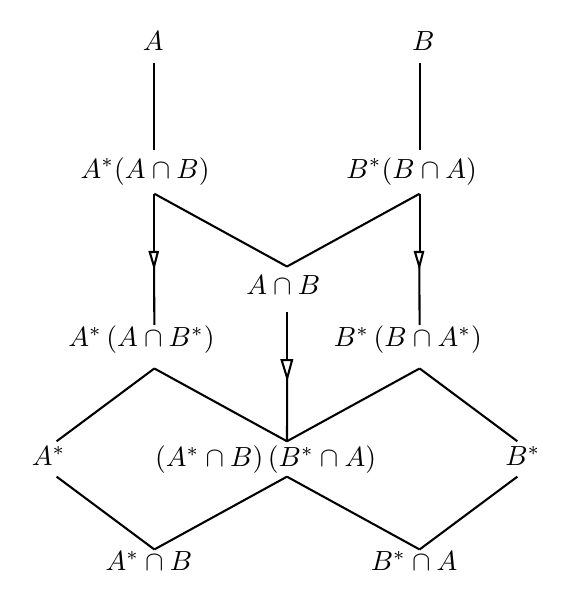
\begin{tikzpicture}[x=0.75pt,y=0.75pt,yscale=-1,xscale=1]
%uncomment if require: \path (0,476); %set diagram left start at 0, and has height of 476

%Straight Lines [id:da1285470564836515] 
\draw    (260.84,147.64) -- (260.84,189.73) ;
%Straight Lines [id:da05078319732728209] 
\draw    (388.64,147.64) -- (388.64,189.73) ;
%Straight Lines [id:da09780746468402302] 
\draw    (260.84,210.77) -- (324.74,245.85) ;
%Straight Lines [id:da17745847701647044] 
\draw    (388.64,210.77) -- (324.74,245.85) ;
%Straight Lines [id:da5095576644106456] 
\draw    (260.84,210.77) -- (260.84,238.84) ;
%Shape: Triangle [id:dp5891558957390246] 
\draw   (260.7,245.85) -- (258.6,238.84) -- (262.52,238.84) -- cycle ;
%Straight Lines [id:da7840217059124364] 
\draw    (260.7,245.85) -- (260.84,273.91) ;
%Straight Lines [id:da40595121864678196] 
\draw    (388.64,210.77) -- (388.64,238.84) ;
%Shape: Triangle [id:dp4463057230026377] 
\draw   (388.5,245.85) -- (386.4,238.84) -- (390.32,238.84) -- cycle ;
%Straight Lines [id:da9773677511142567] 
\draw    (388.5,245.85) -- (388.64,273.91) ;
%Straight Lines [id:da3598676892182031] 
\draw    (324.74,267.78) -- (324.74,290.92) ;
%Straight Lines [id:da7359728450021898] 
\draw    (260.84,294.96) -- (324.74,330.04) ;
%Straight Lines [id:da9152351124333524] 
\draw    (388.64,294.96) -- (324.74,330.04) ;
%Straight Lines [id:da7071342895580122] 
\draw    (213.75,330.04) -- (260.84,294.96) ;
%Straight Lines [id:da7370646140530484] 
\draw    (388.64,294.96) -- (435.73,330.04) ;
%Straight Lines [id:da6592447901565566] 
\draw    (213.75,347.09) -- (260.84,382.16) ;
%Straight Lines [id:da830254473944666] 
\draw    (388.64,382.16) -- (435.73,347.09) ;
%Straight Lines [id:da9011367137466262] 
\draw    (324.74,347.09) -- (260.84,382.16) ;
%Straight Lines [id:da7677251177508744] 
\draw    (324.74,347.09) -- (388.64,382.16) ;
%Shape: Triangle [id:dp47542625091877366] 
\draw   (324.85,299.6) -- (322.15,290.91) -- (327.19,290.91) -- cycle ;
%Straight Lines [id:da12771942521241186] 
\draw    (324.85,299.6) -- (324.74,330.04) ;

% Text Node
\draw (253.84,131.27) node [anchor=north west][inner sep=0.75pt]    {$A$};
% Text Node
\draw (383.48,131.27) node [anchor=north west][inner sep=0.75pt]    {$B$};
% Text Node
\draw (223.84,191.71) node [anchor=north west][inner sep=0.75pt]    {$A^{*}( A\cap B)$};
% Text Node
\draw (351.88,191.71) node [anchor=north west][inner sep=0.75pt]    {$B^{*}( B\cap A)$};
% Text Node
\draw (303.66,248.78) node [anchor=north west][inner sep=0.75pt]    {$A\cap B$};
% Text Node
\draw (217.92,272.84) node [anchor=north west][inner sep=0.75pt]    {$A^{*}\left( A\cap B^{*}\right)$};
% Text Node
\draw (345.88,272.84) node [anchor=north west][inner sep=0.75pt]    {$B^{*}\left( B\cap A^{*}\right)$};
% Text Node
\draw (259.74,330.72) node [anchor=north west][inner sep=0.75pt]    {$\left( A^{*} \cap B\right)\left( B^{*} \cap A\right)$};
% Text Node
\draw (200.31,331.15) node [anchor=north west][inner sep=0.75pt]    {$A^{*}$};
% Text Node
\draw (428.41,331.15) node [anchor=north west][inner sep=0.75pt]    {$B^{*}$};
% Text Node
\draw (235.84,381.52) node [anchor=north west][inner sep=0.75pt]    {$A^{*} \cap B$};
% Text Node
\draw (363.64,381.52) node [anchor=north west][inner sep=0.75pt]    {$B^{*} \cap A$};


\end{tikzpicture}
\end{center}
The subgroups are trivial. Also observed that 
$$
A^*\left( A\cap B^* \right) \cap \left( A\cap B \right) =\left( A^*\cap B \right) \left( B^*\cap A \right) =\left( A\cap B \right) \cap \left( A^*\cap B \right) B^*
$$
and 
$$
A^*\cap \left( A^*\cap B \right) \left( B^*\cap A \right) =A^*\cap B,B^*\cap \left( B^*\cap A \right) \left( A^*\cap B \right) =B^*\cap A,
$$
we have the intersections to be true. Now for the normal subgroups, we observe that 
$$
B^*\lhd B\Rightarrow B\cap B^*\lhd A\cap B\Rightarrow A^*\left( A\cap B^* \right) \lhd A^*\left( A\cap B \right) 
$$
and 
$$
A^*\lhd A\Rightarrow A\cap A^*\lhd A\cap B\Rightarrow B^*\left( B\cap A^* \right) \lhd B^*\left( A\cap B \right) ,
$$
hence the normal subgroups are true. Now consider the parallelogram in the diagram, we have isomorphisms by the Second Isomorphism Theorem: 
$$
A^*\left( A\cap B \right) /A^*\left( A\cap B^* \right) \cong B^*\left( A\cap B \right) /B^*\left( A^*\cap B \right) \cong \left( A\cap B \right) /\left( A^*\cap B \right) \left( B^*\cap A \right) .
$$
\end{proof}
\begin{note}\em
This lemma has another name of the \textbf{Butterfly Lemma}, since the diagram above is similar to a butterfly.
\end{note}
\begin{theorem}(Schreier)
Any two subnormal [resp.normal] series of a group $G$ has subnormal [resp.normal] refinements that are equivalent.
\end{theorem}
\begin{proof}
Let $G=G_0>G_1>\cdots >G_n$ and $G=H_0>H_1>\cdots >H_m$ be two subnormal [resp.normal] series of $G$. For all $0\le i\le n$ consider the following series: 
$$
G_i=G_{i+1}\left( G_i\cap H_0 \right) >G_{i+1}\left( G_i\cap H_1 \right) >\cdots >G_{i+1}\left( G_i\cap H_m \right) >G_{i+1}\left( G_i\cap H_{m+1} \right) =G_{i+1},
$$
where $G_{n+1}=H_{m+1}=\left< e \right> $, then by Zassenhaus' Lemma we have $G_{i+1}\left( G_i\cap H_{j+1} \right) \lhd G_{i+1}\left( G_i\cap H_j \right) $ [if the original series are normal, then observe that $G_i\lhd G,H_j\lhd G\Rightarrow G_i\cap H_j\lhd G$, $G_{i+1}\lhd G$ and $G_{i+1}\left( G_i\cap H_j \right) =G_{i+1}\lor \left( G_i\cap H_j \right) \lhd G$]. Inserting these groups between $G_i$ and $G_{i+1}$ for all $0\le i\le n$, and denote $G\left( i,j \right) =G_{i+1}\left( G_i\cap H_j \right) $, we have 
$$
G=G\left( 0,0 \right) >G\left( 0,1 \right) >\cdots >G\left( 0,m \right) >\cdots >G\left( n,0 \right) >\cdots >G\left( n,m \right) .
$$
Similarly we may have the refinement of $G=H_0>H_1>\cdots >H_m$ as 
$$
G=H\left( 0,0 \right) >H\left( 1,0 \right) >\cdots >H\left( n,0 \right) >\cdots >H\left( 0,m \right) >\cdots >H\left( n,m \right) ,
$$
It is easy to see that the two series above has the same number of terms $(n+1)(m+1)$. For each pair $(i,j)$ again by Zassenhaus' Lemma we have 
$$
\frac{G\left( i,j \right)}{G\left( i,j+1 \right)}=\frac{G_{i+1}\left( G_i\cap H_j \right)}{G_{i+1}\left( G_i\cap H_{j+1} \right)}\cong \frac{H_{j+1}\left( G_i\cap H_j \right)}{H_{j+1}\left( G_{i+1}\cap H_j \right)}=\frac{H\left( i,j \right)}{H\left( i+1,j \right)},
$$
therefore we finished our proof.
\end{proof}
\begin{theorem}(Jordan-Holder)
Any two composition series of a group $G$ are equivalent. Therefore every group having a composition series determines a unique list of simple groups.
\end{theorem}
\begin{proof}
Since composition series are subnormal series, by Schreier's Theorem we know that every two composition series have equivalent refinements. But every refinement of a composition series is equivalent to itself, then any two composition series are equivalent.
\end{proof}
\begin{note}\em
The theorem does not state the existence of a composition series for a given group.
\end{note}
The Jordan-Holder Theorem indicates that some knowledge of simple groups might be useful. The classification of all finite simple groups have been finished in 1981, which is based on the work of a large number of group theorists. We may note that non-abelian simple groups of small order are quite rare. There are only two non-abelian simple groups of order less than 200: $A_5$ and a subgroup of $S_7$ of order $168$.
\begin{center}
\begin{large}
    \textbf{Exercises for 3.6}
\end{large}
\end{center}
\begin{problem}\em
If $G=G_0>G_1>\cdots>G_n$ is a subnormal series of a finite group $G$, then $|G|=\left(\prod_{i=0}^{n-1}|G_i/G_{i+1}|\right)|G_n|$.
\end{problem}
\begin{proof}
We observed that 
$$
\left( \prod_{i=0}^{n-1}{\left| G_i/G_{i+1} \right|} \right) \left| G_n \right|=\left( \prod_{i=0}^{n-1}{\left[ G_i:G_{i+1} \right]} \right) \left| G_n \right|=\left[ G_0:G_n \right] \left| G_n \right|=\left| G_0 \right|=\left| G \right|.
$$
\end{proof}
\begin{problem}\em
If $N$ is a simple normal subgroup of a group $G$ and $G/N$ has a composition series, then $G$ has a composition series.
\end{problem}
\begin{proof}
Consider the composition series $G/N=G_0/N>G_1/N>\cdots >G_n/N=\left< e_{G/N} \right> $, from which we have a subnormal series of $G$, which is $G=G_0>G_1>\cdots >G_n$. By the Third Isomorphism Theorem we have $G_i/G_{i+1}\cong \left( G_i/N \right) /\left( G_{i+1}/N \right) $ is a simple group, therefore the series $G=G_0>G_1>\cdots >G_n$ is a composition series.
\end{proof}
\begin{problem}\em
A composition series of a group is a subnormal series of maximal (finite) length.
\end{problem}
\begin{proof}
Let $G$ be a group and $G=G_0>G_1>\cdots >G_n$ be a composition series of $G$. If there exists some series $G=G_0^\prime>G_1^\prime>\cdots >G_m^\prime$ whose length is longer than $G=G_0>G_1>\cdots >G_n$, then the new series is a refinement of the original series. However the refinement of a composition series is equivalent to itself, which is a contradict!
\end{proof}
\begin{problem}\em
An abelian group has a composition series if and only if it is finite.
\end{problem}
\begin{proof}
Let $G$ be a finite abelian group, Then it is finite and hence has a composition series. Conversely, let $G$ be an abelian group and $G=G_0>G_1>\cdots>G_n$ be a composition series of $G$. Then each $G_i/G_{i+1}$ is abelian and simple, therefore it is finite cyclic and has prime order. By exercise 3.60 we may conclude that $G$ is finite, therefore $G$ is finite abelian.
\end{proof}
\begin{problem}\em
If $H\lhd G$, where $G$ has a composition series, then $G$ has a composition series one of whose terms is $H$.
\end{problem}
\begin{proof}
Let $G=G_0>G_1>\cdots >G_n$ be a composition series of $G$. Then consider the normal series $G>H>\left< e \right> $, which is either or not a composition series. If it is a composition series, then we are done. If not, by Schreier's Theorem we have a subnormal series $G=N_0>N_1>\cdots >N_r=\left< e \right> $ which is a refinement of both $G=G_0>G_1>\cdots >G_n$ and $G>H>\left< e \right> $. Clearly there exists some $N_i=H$. Now we show that the new series is a composition series. Note that there is no proper refinement of a composition series and hence $G=N_0>N_1>\cdots >N_r=\left< e \right> $ is equivalent to the original series and we finished our proof.
\end{proof}
\begin{problem}\em
A solvable group with a composition series is finite.
\end{problem}
\begin{proof}
Let $G$ be a solvable group and $G=G_0>G_1>\cdots >G_n$ be a composition series. Since $G$ is solvable, it has a solvable series $G=H_0>H_1>\cdots >H_m$. Consider the refinement of these two series, which is equivalent by Schreier's Theorem. We denote the new series as $G=N_0>N_1>\cdots >N_r$, which is the refinement of a solvable series and hence solvable. Also it is the refinement of a composition series, which is equivalent to itself. Therefore the new series is both composition and solvable series, hence $N_i/N_{i+1}$ is abelian and simple, therefore isomorphic to cyclic group of prime order. By exercise 3.60 we know that $G$ is of finite order.
\end{proof}
\begin{problem}\em
If $H$ and $K$ are solvable subgroups of $G$ with $H\lhd G$, then $HK$ is a solvable subgroup of $G$.
\end{problem}
\begin{proof}
By Theorem 3.46 we know that $G$ is solvable if and only if $N$ and $G/N$ is solvable, where $N$ is normal in $G$. Now consider $HK$. Clearly $H\lhd HK$, and by the Second Isomorphism Theorem we have $HK/K\cong H/(H\cap K)$, which is solvable since every quotient and subgroup of a solvable group is also solvable. Therefore $HK$ is solvable by Theorem 3.46.
\end{proof}
\begin{problem}\em
A group $G$ is nilpotent if and only if there is a normal series $G=G_0>G_1>\cdots>G_n=\left<e\right>$ such that $G_i/G_{i+1}<C(G/G_{i+1})$ for every $i$.
\end{problem}
\begin{proof}
If $G$ is nilpotent, we have shown that $C_i\left( G \right) /C_{i+1}\left( G \right) =C\left( G/C_{i+1}\left( G \right) \right) $, which its central chain is a normal series satisfies the condition. Conversely, let $\left< e \right> <G_1<G_2<\cdots <G_n$ be a normal series with $G_i/G_{i-1}<C\left( G/G_{i-1} \right) $, we show that $G$ is nilpotent by proving $G_i<C_i\left( G \right) $ by induction. For $i=1$, we observe $G_1=G_1/G_0<C\left( G/G_0 \right) =C\left( G \right) =C_1\left( G \right) $ and the result holds. Now suppose this is true for $k$, now consider $k+1$. Define the map $G/G_{k}\to G/C_k(G)$ and consider the image of $C(G/G_k)$, which maps into $C_{k+1}(G)/C_k(G)$. Thus every element in $G_{k+1}$ maps into $C_{k+1}(G)$ and we finished our proof.
\end{proof}
\begin{problem}\em
Prove the Fundamental Theorem of Arithmetic by Jordan-Holder's Theorem.
\end{problem}
\begin{proof}
Let $n=p_1p_2\cdots p_k=q_1q_2\cdots q_s$. We show that for all $i$ there exists some $j$ such that $p_i=q_j$. We observe the following composition series: 
$$
\mathbb{Z} /n\mathbb{Z} >\mathbb{Z} /\left( \frac{n}{p_1} \right) \mathbb{Z} >\mathbb{Z} /\left( \frac{n}{p_1p_2} \right) \mathbb{Z} >\cdots >\mathbb{Z} /\left( \frac{n}{p_1p_2\cdots p_k} \right) \mathbb{Z} =\left\{ 1 \right\} 
$$
and 
$$
\mathbb{Z} /n\mathbb{Z} >\mathbb{Z} /\left( \frac{n}{q_1} \right) \mathbb{Z} >\mathbb{Z} /\left( \frac{n}{q_1q_2} \right) \mathbb{Z} >\cdots >\mathbb{Z} /\left( \frac{n}{q_1q_2\cdots q_s} \right) \mathbb{Z} =\left\{ 1 \right\} ,
$$
which are suppose to be equivalent by Jordan-Holder's Theorem, therefore the composition of the integer $n$ is unique and we finished our proof.
\end{proof}
\subsection{Postscript on Group Theory}
We end our discussion in group theory with a full classification of groups of small order. We only present the classification of groups with orders $\leq 15$ (as shown in the table below). In the "Reference" column, "[G]Corollary 6.2" refers to Corollary 6.2 in GTM73, while the other entries without [G] indicate references to the main text of the notes.
$$
\begin{matrix}
	\mathrm{Order}&		\mathrm{Distinct} \mathrm{Groups}&		\mathrm{Reference}\\
	1&		\left< e \right>&		\cdots\\
	2&		\mathbb{Z} _2&		\mathrm{Exercise}2.42\\
	3&		\mathbb{Z} _3&		\mathrm{Exercise}2.42\\
	4&		\mathbb{Z} _4,\mathbb{Z} _2\oplus \mathbb{Z} _2&		\mathrm{Exercise}2.44\\
	5&		\mathbb{Z} _5&		\mathrm{Exercise}2.42\\
	6&		\mathbb{Z} _6,D_3&		\left[ \mathrm{G} \right] \mathrm{Corollary}6.2\\
	7&		\mathbb{Z} _7&		\mathrm{Exercise}2.42\\
	8&		\mathbb{Z} _2\oplus \mathbb{Z} _2\oplus \mathbb{Z} _2,\mathbb{Z} _2\oplus \mathbb{Z} _4,\mathbb{Z} _8,Q_8,D_4&		\mathrm{Theorem}3.7,\left[ \mathrm{G} \right] \mathrm{Corollary}6.2\\
	9&		\mathbb{Z} _3\oplus \mathbb{Z} _3,\mathbb{Z} _9&		\mathrm{Exercise}3.51,\left[ \mathrm{G} \right] \mathrm{Corollary}6.2\\
	10&		\mathbb{Z} _{10},D_5&		\mathrm{Theorem}3.7\\
	11&		\mathbb{Z} _{11}&		\mathrm{Exercise}2.42\\
	12&		\mathbb{Z} _2\oplus \mathbb{Z} _6,\mathbb{Z} _{12},A_4,D_6,T&		\mathrm{Theorem}3.7,\left[ \mathrm{G} \right] \mathrm{Proposition}6.4\\
	13&		\mathbb{Z} _{13}&		\mathrm{Exercise}2.42\\
	14&		\mathbb{Z} _{14},D_7&		\left[ \mathrm{G} \right] \mathrm{Corollary}6.2\\
	15&		\mathbb{Z} _{15}&		\left[ \mathrm{G} \right] \mathrm{Proposition}6.1\\
\end{matrix}
$$